\documentclass[twoside]{book}

% Packages required by doxygen
\usepackage{fixltx2e}
\usepackage{calc}
\usepackage{doxygen}
\usepackage[export]{adjustbox} % also loads graphicx
\usepackage{graphicx}
\usepackage[utf8]{inputenc}
\usepackage{makeidx}
\usepackage{multicol}
\usepackage{multirow}
\PassOptionsToPackage{warn}{textcomp}
\usepackage{textcomp}
\usepackage[nointegrals]{wasysym}
\usepackage[table]{xcolor}

% Font selection
\usepackage[T1]{fontenc}
\usepackage[scaled=.90]{helvet}
\usepackage{courier}
\usepackage{amssymb}
\usepackage{sectsty}
\renewcommand{\familydefault}{\sfdefault}
\allsectionsfont{%
  \fontseries{bc}\selectfont%
  \color{darkgray}%
}
\renewcommand{\DoxyLabelFont}{%
  \fontseries{bc}\selectfont%
  \color{darkgray}%
}
\newcommand{\+}{\discretionary{\mbox{\scriptsize$\hookleftarrow$}}{}{}}

% Page & text layout
\usepackage{geometry}
\geometry{%
  a4paper,%
  top=2.5cm,%
  bottom=2.5cm,%
  left=2.5cm,%
  right=2.5cm%
}
\tolerance=750
\hfuzz=15pt
\hbadness=750
\setlength{\emergencystretch}{15pt}
\setlength{\parindent}{0cm}
\setlength{\parskip}{3ex plus 2ex minus 2ex}
\makeatletter
\renewcommand{\paragraph}{%
  \@startsection{paragraph}{4}{0ex}{-1.0ex}{1.0ex}{%
    \normalfont\normalsize\bfseries\SS@parafont%
  }%
}
\renewcommand{\subparagraph}{%
  \@startsection{subparagraph}{5}{0ex}{-1.0ex}{1.0ex}{%
    \normalfont\normalsize\bfseries\SS@subparafont%
  }%
}
\makeatother

% Headers & footers
\usepackage{fancyhdr}
\pagestyle{fancyplain}
\fancyhead[LE]{\fancyplain{}{\bfseries\thepage}}
\fancyhead[CE]{\fancyplain{}{}}
\fancyhead[RE]{\fancyplain{}{\bfseries\leftmark}}
\fancyhead[LO]{\fancyplain{}{\bfseries\rightmark}}
\fancyhead[CO]{\fancyplain{}{}}
\fancyhead[RO]{\fancyplain{}{\bfseries\thepage}}
\fancyfoot[LE]{\fancyplain{}{}}
\fancyfoot[CE]{\fancyplain{}{}}
\fancyfoot[RE]{\fancyplain{}{\bfseries\scriptsize Generated by Doxygen }}
\fancyfoot[LO]{\fancyplain{}{\bfseries\scriptsize Generated by Doxygen }}
\fancyfoot[CO]{\fancyplain{}{}}
\fancyfoot[RO]{\fancyplain{}{}}
\renewcommand{\footrulewidth}{0.4pt}
\renewcommand{\chaptermark}[1]{%
  \markboth{#1}{}%
}
\renewcommand{\sectionmark}[1]{%
  \markright{\thesection\ #1}%
}

% Indices & bibliography
\usepackage{natbib}
\usepackage[titles]{tocloft}
\setcounter{tocdepth}{3}
\setcounter{secnumdepth}{5}
\makeindex

% Hyperlinks (required, but should be loaded last)
\usepackage{ifpdf}
\ifpdf
  \usepackage[pdftex,pagebackref=true]{hyperref}
\else
  \usepackage[ps2pdf,pagebackref=true]{hyperref}
\fi
\hypersetup{%
  colorlinks=true,%
  linkcolor=blue,%
  citecolor=blue,%
  unicode%
}

% Custom commands
\newcommand{\clearemptydoublepage}{%
  \newpage{\pagestyle{empty}\cleardoublepage}%
}

\usepackage{caption}
\captionsetup{labelsep=space,justification=centering,font={bf},singlelinecheck=off,skip=4pt,position=top}

%===== C O N T E N T S =====

\begin{document}

% Titlepage & ToC
\hypersetup{pageanchor=false,
             bookmarksnumbered=true,
             pdfencoding=unicode
            }
\pagenumbering{alph}
\begin{titlepage}
\vspace*{7cm}
\begin{center}%
{\Large My Project }\\
\vspace*{1cm}
{\large Generated by Doxygen 1.8.14}\\
\end{center}
\end{titlepage}
\clearemptydoublepage
\pagenumbering{roman}
\tableofcontents
\clearemptydoublepage
\pagenumbering{arabic}
\hypersetup{pageanchor=true}

%--- Begin generated contents ---
\chapter{My Personal Index Page}
\label{index}\hypertarget{index}{}\hypertarget{index_intro_sec}{}\section{Introduction}\label{index_intro_sec}
This is a school project! The school assignemt is called I\+P\+A\+S\+S(\+Individual Propedeuse Assessment). The whole project can be found here\+: \href{https://github.com/YouriMulder/IPASS_2018}{\tt https\+://github.\+com/\+Youri\+Mulder/\+I\+P\+A\+S\+S\+\_\+2018}. ~\newline
 ~\newline
 The libraries are written on top of H\+W\+L\+IB and B\+M\+P\+TK. ~\newline
 Special thanks to (c) Wouter van Ooijen (\href{mailto:wouter@voti.nl}{\tt wouter@voti.\+nl}) 2017 for creating the Arduino Due toolchain. ~\newline
 H\+W\+L\+IB (hardware library)\+: \href{https://github.com/wovo/hwlib}{\tt https\+://github.\+com/wovo/hwlib} ~\newline
 B\+M\+P\+TK (Bare Metal Programming Tool Kit)\+: \href{https://github.com/wovo/bmptk}{\tt https\+://github.\+com/wovo/bmptk} ~\newline
 Before installing my software you should\textquotesingle{}ve installed B\+M\+P\+Tk and H\+W\+L\+IB. My libraries D\+ON\textquotesingle{}T work without H\+W\+L\+IB and B\+M\+P\+TK ~\newline
 \hypertarget{index_license_sec}{}\section{Boost License\+:}\label{index_license_sec}
Distributed under the Boost Software License, Version 1.\+0. (See accompanying file L\+I\+C\+E\+N\+S\+E\+\_\+1\+\_\+0.\+txt or copy at \href{http://www.boost.org/LICENSE_1_0.txt}{\tt http\+://www.\+boost.\+org/\+L\+I\+C\+E\+N\+S\+E\+\_\+1\+\_\+0.\+txt})\hypertarget{index_requirements_sec}{}\section{Requirements}\label{index_requirements_sec}
H\+W\+L\+IB (hardware library)\+: \href{https://github.com/wovo/hwlib}{\tt https\+://github.\+com/wovo/hwlib} ~\newline
 B\+M\+P\+TK (Bare Metal Programming Tool Kit)\+: \href{https://github.com/wovo/bmptk}{\tt https\+://github.\+com/wovo/bmptk}~\newline
 Codelite I\+DE (recommended! not necessary)\+: \href{https://codelite.org/}{\tt https\+://codelite.\+org/}\hypertarget{index_install_sec}{}\section{Installation}\label{index_install_sec}
After installing H\+W\+L\+IB and B\+M\+P\+TK you have to clone my github repo\+: \href{https://github.com/YouriMulder/IPASS_2018}{\tt https\+://github.\+com/\+Youri\+Mulder/\+I\+P\+A\+S\+S\+\_\+2018}. Choose the library you want to use in the Libraries folder. After choosing the library you should test if your chip is working correctly. (check the testing section)\hypertarget{index_import_sec}{}\section{Import library to your own project}\label{index_import_sec}
To use a library in your own project you should just copy the folder or files to the directory of your own projected and add the files to your makefile (Note that you need H\+W\+L\+IB and B\+M\+P\+TK for using the libraries!).\hypertarget{index_test_sec}{}\section{Testing}\label{index_test_sec}
When you want to test the libraries or your chip you need to run the main.\+cpp located in the folder of the library.\hypertarget{index_author_sec}{}\section{Author}\label{index_author_sec}
The project is made by\+: Youri Mulder -\/ Computer science year 1 (Hogeschool Utrecht)

reeferences\+\_\+sec Used sites/datasheets \href{https://www.mpja.com/download/31227sc.pdf}{\tt https\+://www.\+mpja.\+com/download/31227sc.\+pdf} \href{https://datasheets.maximintegrated.com/en/ds/DS3231.pdf}{\tt https\+://datasheets.\+maximintegrated.\+com/en/ds/\+D\+S3231.\+pdf} \href{https://www.nxp.com/docs/en/data-sheet/MF1S50YYX_V1.pdf}{\tt https\+://www.\+nxp.\+com/docs/en/data-\/sheet/\+M\+F1\+S50\+Y\+Y\+X\+\_\+\+V1.\+pdf} \href{https://www.nxp.com/docs/en/data-sheet/MFRC522.pdf}{\tt https\+://www.\+nxp.\+com/docs/en/data-\/sheet/\+M\+F\+R\+C522.\+pdf} \href{http://www.radio-electronics.com/info/wireless/nfc/near-field-communications-modulation-rf-signal-interface.php}{\tt http\+://www.\+radio-\/electronics.\+com/info/wireless/nfc/near-\/field-\/communications-\/modulation-\/rf-\/signal-\/interface.\+php} \href{http://www.nedapidentification.com/news/insights/understanding-the-confusing-world-of-rfid-tags-and-readers-in-access-control.html}{\tt http\+://www.\+nedapidentification.\+com/news/insights/understanding-\/the-\/confusing-\/world-\/of-\/rfid-\/tags-\/and-\/readers-\/in-\/access-\/control.\+html} 
\chapter{R\+E\+A\+D\+ME}
\label{md__r_e_a_d_m_e}
\Hypertarget{md__r_e_a_d_m_e}
/$\ast$! 
\chapter{Module Index}
\section{Modules}
Here is a list of all modules\+:\begin{DoxyCompactList}
\item \contentsline{section}{Bit\+Parser}{\pageref{group__bit_parser}}{}
\end{DoxyCompactList}

\chapter{Hierarchical Index}
\section{Class Hierarchy}
This inheritance list is sorted roughly, but not completely, alphabetically\+:\begin{DoxyCompactList}
\item \contentsline{section}{alarm}{\pageref{classalarm}}{}
\item \contentsline{section}{buzzer}{\pageref{classbuzzer}}{}
\item \contentsline{section}{display\+Manager}{\pageref{classdisplay_manager}}{}
\item i2c\+\_\+bus\+\_\+bit\+\_\+banged\+\_\+scl\+\_\+sda\begin{DoxyCompactList}
\item \contentsline{section}{i2c\+Bus}{\pageref{classi2c_bus}}{}
\end{DoxyCompactList}
\item \contentsline{section}{motion\+Sensor}{\pageref{classmotion_sensor}}{}
\begin{DoxyCompactList}
\item \contentsline{section}{H\+C\+S\+R501}{\pageref{class_h_c_s_r501}}{}
\end{DoxyCompactList}
\item \contentsline{section}{personal\+Data}{\pageref{structpersonal_data}}{}
\item \contentsline{section}{rfid}{\pageref{classrfid}}{}
\begin{DoxyCompactList}
\item \contentsline{section}{M\+F\+R\+C522}{\pageref{class_m_f_r_c522}}{}
\end{DoxyCompactList}
\item spi\+\_\+bus\+\_\+bit\+\_\+banged\+\_\+sclk\+\_\+mosi\+\_\+miso\begin{DoxyCompactList}
\item \contentsline{section}{spi\+Bus}{\pageref{classspi_bus}}{}
\end{DoxyCompactList}
\item \contentsline{section}{time}{\pageref{classtime}}{}
\begin{DoxyCompactList}
\item \contentsline{section}{real\+Time\+Clock}{\pageref{classreal_time_clock}}{}
\begin{DoxyCompactList}
\item \contentsline{section}{D\+S3231}{\pageref{class_d_s3231}}{}
\end{DoxyCompactList}
\item \contentsline{section}{timestamp}{\pageref{classtimestamp}}{}
\end{DoxyCompactList}
\end{DoxyCompactList}

\chapter{Class Index}
\section{Class List}
Here are the classes, structs, unions and interfaces with brief descriptions\+:\begin{DoxyCompactList}
\item\contentsline{section}{\mbox{\hyperlink{classalarm}{alarm}} }{\pageref{classalarm}}{}
\item\contentsline{section}{\mbox{\hyperlink{classbuzzer}{buzzer}} }{\pageref{classbuzzer}}{}
\item\contentsline{section}{\mbox{\hyperlink{classdisplay_manager}{display\+Manager}} }{\pageref{classdisplay_manager}}{}
\item\contentsline{section}{\mbox{\hyperlink{class_d_s3231}{D\+S3231}} }{\pageref{class_d_s3231}}{}
\item\contentsline{section}{\mbox{\hyperlink{class_h_c_s_r501}{H\+C\+S\+R501}} }{\pageref{class_h_c_s_r501}}{}
\item\contentsline{section}{\mbox{\hyperlink{classi2c_bus}{i2c\+Bus}} \\*Basic I2C functions like write and read a register }{\pageref{classi2c_bus}}{}
\item\contentsline{section}{\mbox{\hyperlink{class_m_f_r_c522}{M\+F\+R\+C522}} }{\pageref{class_m_f_r_c522}}{}
\item\contentsline{section}{\mbox{\hyperlink{classmotion_sensor}{motion\+Sensor}} }{\pageref{classmotion_sensor}}{}
\item\contentsline{section}{\mbox{\hyperlink{structpersonal_data}{personal\+Data}} }{\pageref{structpersonal_data}}{}
\item\contentsline{section}{\mbox{\hyperlink{classreal_time_clock}{real\+Time\+Clock}} }{\pageref{classreal_time_clock}}{}
\item\contentsline{section}{\mbox{\hyperlink{classrfid}{rfid}} }{\pageref{classrfid}}{}
\item\contentsline{section}{\mbox{\hyperlink{classspi_bus}{spi\+Bus}} \\*Basic S\+PI functions like write and read a register }{\pageref{classspi_bus}}{}
\item\contentsline{section}{\mbox{\hyperlink{classtime}{time}} }{\pageref{classtime}}{}
\item\contentsline{section}{\mbox{\hyperlink{classtimestamp}{timestamp}} }{\pageref{classtimestamp}}{}
\end{DoxyCompactList}

\chapter{Module Documentation}
\hypertarget{group__bit_parser}{}\section{Bit\+Parser}
\label{group__bit_parser}\index{Bit\+Parser@{Bit\+Parser}}
\subsection*{Functions}
\begin{DoxyCompactItemize}
\item 
void \mbox{\hyperlink{group__bit_parser_ga59838a77502d6d7f71258ff348055510}{bit\+Parser\+::print\+Byte}} (uint8\+\_\+t byte)
\begin{DoxyCompactList}\small\item\em Print a byte to the console. \end{DoxyCompactList}\item 
void \mbox{\hyperlink{group__bit_parser_ga25b5179d0eec3cf5d3f465c7b2c179b6}{bit\+Parser\+::print\+Bytes}} (uint16\+\_\+t bytes)
\begin{DoxyCompactList}\small\item\em Print a two bytes to the console. \end{DoxyCompactList}\item 
uint8\+\_\+t \mbox{\hyperlink{group__bit_parser_gad207f006665a21b8cbdb0148d81b80c1}{bit\+Parser\+::\+B\+C\+D\+To\+D\+EC}} (uint8\+\_\+t B\+CD)
\begin{DoxyCompactList}\small\item\em Turn a B\+C\+D-\/coded value into a decimal value. \end{DoxyCompactList}\item 
uint8\+\_\+t \mbox{\hyperlink{group__bit_parser_gabf889c80952fe124c224fd61c59704d1}{bit\+Parser\+::\+D\+E\+C\+To\+B\+CD}} (uint8\+\_\+t D\+EC)
\begin{DoxyCompactList}\small\item\em Turn a decimal value into a B\+C\+D-\/coded value. \end{DoxyCompactList}\item 
int \mbox{\hyperlink{group__bit_parser_ga2cdf3099581569732367d0fc965e0a7e}{bit\+Parser\+::uint8\+\_\+t\+To\+Int}} (uint8\+\_\+t byte)
\begin{DoxyCompactList}\small\item\em Turn a uint8\+\_\+t into a signed integer. \end{DoxyCompactList}\end{DoxyCompactItemize}
\subsection*{Variables}
\begin{DoxyCompactItemize}
\item 
\mbox{\Hypertarget{group__bit_parser_ga1089bf9f6a8c7710cb6f4161697d437c}\label{group__bit_parser_ga1089bf9f6a8c7710cb6f4161697d437c}} 
const int \mbox{\hyperlink{group__bit_parser_ga1089bf9f6a8c7710cb6f4161697d437c}{bit\+Parser\+::n\+Bitsin\+Byte}} = 8
\begin{DoxyCompactList}\small\item\em Mask for a whole byte. \end{DoxyCompactList}\item 
\mbox{\Hypertarget{group__bit_parser_ga47dacd6f8d9409a4866c9e22f8e0a3ca}\label{group__bit_parser_ga47dacd6f8d9409a4866c9e22f8e0a3ca}} 
const int \mbox{\hyperlink{group__bit_parser_ga47dacd6f8d9409a4866c9e22f8e0a3ca}{bit\+Parser\+::n\+Bitsin\+Half\+A\+Byte}} = 4
\begin{DoxyCompactList}\small\item\em Mask for half of a byte. \end{DoxyCompactList}\item 
\mbox{\Hypertarget{group__bit_parser_ga3706423b79d72421f8796475baf10c27}\label{group__bit_parser_ga3706423b79d72421f8796475baf10c27}} 
const uint8\+\_\+t \mbox{\hyperlink{group__bit_parser_ga3706423b79d72421f8796475baf10c27}{bit\+Parser\+::left\+Half\+Byte\+Mask}} = 0x78
\begin{DoxyCompactList}\small\item\em Mask for the 4 left bits of a byte. \end{DoxyCompactList}\item 
\mbox{\Hypertarget{group__bit_parser_gaadb1b05603363dca189d9f3900cebce4}\label{group__bit_parser_gaadb1b05603363dca189d9f3900cebce4}} 
const uint8\+\_\+t \mbox{\hyperlink{group__bit_parser_gaadb1b05603363dca189d9f3900cebce4}{bit\+Parser\+::right\+Halfg\+Byte\+Mask}} = 0xF
\begin{DoxyCompactList}\small\item\em Mask for the 4 right bits of a byte. \end{DoxyCompactList}\end{DoxyCompactItemize}


\subsection{Detailed Description}


\subsection{Function Documentation}
\mbox{\Hypertarget{group__bit_parser_gad207f006665a21b8cbdb0148d81b80c1}\label{group__bit_parser_gad207f006665a21b8cbdb0148d81b80c1}} 
\index{Bit\+Parser@{Bit\+Parser}!B\+C\+D\+To\+D\+EC@{B\+C\+D\+To\+D\+EC}}
\index{B\+C\+D\+To\+D\+EC@{B\+C\+D\+To\+D\+EC}!Bit\+Parser@{Bit\+Parser}}
\subsubsection{\texorpdfstring{B\+C\+D\+To\+D\+E\+C()}{BCDToDEC()}}
{\footnotesize\ttfamily uint8\+\_\+t bit\+Parser\+::\+B\+C\+D\+To\+D\+EC (\begin{DoxyParamCaption}\item[{uint8\+\_\+t}]{B\+CD }\end{DoxyParamCaption})}



Turn a B\+C\+D-\/coded value into a decimal value. 


\begin{DoxyParams}{Parameters}
{\em B\+CD} & the B\+C\+D-\/coded value you want to turn into a decimal value. \\
\hline
\end{DoxyParams}
\begin{DoxyReturn}{Returns}
An uint8\+\_\+t containing the decimal value of the B\+C\+D-\/coded value. 
\end{DoxyReturn}
\begin{DoxySeeAlso}{See also}
D\+E\+C\+To\+B\+CD for doing the opposite. 
\end{DoxySeeAlso}
\mbox{\Hypertarget{group__bit_parser_gabf889c80952fe124c224fd61c59704d1}\label{group__bit_parser_gabf889c80952fe124c224fd61c59704d1}} 
\index{Bit\+Parser@{Bit\+Parser}!D\+E\+C\+To\+B\+CD@{D\+E\+C\+To\+B\+CD}}
\index{D\+E\+C\+To\+B\+CD@{D\+E\+C\+To\+B\+CD}!Bit\+Parser@{Bit\+Parser}}
\subsubsection{\texorpdfstring{D\+E\+C\+To\+B\+C\+D()}{DECToBCD()}}
{\footnotesize\ttfamily uint8\+\_\+t bit\+Parser\+::\+D\+E\+C\+To\+B\+CD (\begin{DoxyParamCaption}\item[{uint8\+\_\+t}]{D\+EC }\end{DoxyParamCaption})}



Turn a decimal value into a B\+C\+D-\/coded value. 


\begin{DoxyParams}{Parameters}
{\em D\+EC} & the decimal value you want to turn into a B\+C\+D-\/coded value. \\
\hline
\end{DoxyParams}
\begin{DoxyReturn}{Returns}
An uint8\+\_\+t containing B\+C\+D-\/coded value of the decimal value. 
\end{DoxyReturn}
\begin{DoxySeeAlso}{See also}
B\+C\+Dto\+D\+EC for doing the opposite. 
\end{DoxySeeAlso}
\mbox{\Hypertarget{group__bit_parser_ga59838a77502d6d7f71258ff348055510}\label{group__bit_parser_ga59838a77502d6d7f71258ff348055510}} 
\index{Bit\+Parser@{Bit\+Parser}!print\+Byte@{print\+Byte}}
\index{print\+Byte@{print\+Byte}!Bit\+Parser@{Bit\+Parser}}
\subsubsection{\texorpdfstring{print\+Byte()}{printByte()}}
{\footnotesize\ttfamily void bit\+Parser\+::print\+Byte (\begin{DoxyParamCaption}\item[{uint8\+\_\+t}]{byte }\end{DoxyParamCaption})}



Print a byte to the console. 

The byte is printed with the L\+SB first (left). \begin{DoxyWarning}{Warning}
The byte is printed with the L\+SB first (left). 
\end{DoxyWarning}
\mbox{\Hypertarget{group__bit_parser_ga25b5179d0eec3cf5d3f465c7b2c179b6}\label{group__bit_parser_ga25b5179d0eec3cf5d3f465c7b2c179b6}} 
\index{Bit\+Parser@{Bit\+Parser}!print\+Bytes@{print\+Bytes}}
\index{print\+Bytes@{print\+Bytes}!Bit\+Parser@{Bit\+Parser}}
\subsubsection{\texorpdfstring{print\+Bytes()}{printBytes()}}
{\footnotesize\ttfamily void bit\+Parser\+::print\+Bytes (\begin{DoxyParamCaption}\item[{uint16\+\_\+t}]{bytes }\end{DoxyParamCaption})}



Print a two bytes to the console. 

The bytes are printed with the L\+SB first (left). \begin{DoxyWarning}{Warning}
The byte are printed with the L\+SB first (left). 
\end{DoxyWarning}
\mbox{\Hypertarget{group__bit_parser_ga2cdf3099581569732367d0fc965e0a7e}\label{group__bit_parser_ga2cdf3099581569732367d0fc965e0a7e}} 
\index{Bit\+Parser@{Bit\+Parser}!uint8\+\_\+t\+To\+Int@{uint8\+\_\+t\+To\+Int}}
\index{uint8\+\_\+t\+To\+Int@{uint8\+\_\+t\+To\+Int}!Bit\+Parser@{Bit\+Parser}}
\subsubsection{\texorpdfstring{uint8\+\_\+t\+To\+Int()}{uint8\_tToInt()}}
{\footnotesize\ttfamily int bit\+Parser\+::uint8\+\_\+t\+To\+Int (\begin{DoxyParamCaption}\item[{uint8\+\_\+t}]{byte }\end{DoxyParamCaption})}



Turn a uint8\+\_\+t into a signed integer. 


\begin{DoxyParams}{Parameters}
{\em byte} & the uint8\+\_\+t you want to turn into a signed integer. \\
\hline
\end{DoxyParams}
\begin{DoxyReturn}{Returns}
An signed int containing the signed value of the uint8\+\_\+t. 
\end{DoxyReturn}

\chapter{Class Documentation}
\hypertarget{classalarm}{}\section{alarm Class Reference}
\label{classalarm}\index{alarm@{alarm}}
\subsection*{Public Member Functions}
\begin{DoxyCompactItemize}
\item 
\mbox{\Hypertarget{classalarm_a291b28fcd9ffcdcce8e8fce6e512643f}\label{classalarm_a291b28fcd9ffcdcce8e8fce6e512643f}} 
{\bfseries alarm} (\mbox{\hyperlink{classreal_time_clock}{real\+Time\+Clock}} \&rtc, \mbox{\hyperlink{classrfid}{rfid}} \&rfid\+Reader, \mbox{\hyperlink{classmotion_sensor}{motion\+Sensor}} \&motion\+Detector, \mbox{\hyperlink{classbuzzer}{buzzer}} \&horn, \mbox{\hyperlink{classdisplay_manager}{display\+Manager}} \&d\+Manager, bool is\+Active=false)
\item 
\mbox{\Hypertarget{classalarm_a6077fa2ce42a4b04cb3ebbdff7f112ea}\label{classalarm_a6077fa2ce42a4b04cb3ebbdff7f112ea}} 
bool {\bfseries get\+Is\+Active} ()
\item 
\mbox{\Hypertarget{classalarm_a04d2c03a06c2208e642ab55c2f5d3f17}\label{classalarm_a04d2c03a06c2208e642ab55c2f5d3f17}} 
bool {\bfseries get\+Is\+Ringing} ()
\item 
\mbox{\Hypertarget{classalarm_a32500531a9dc214f564aa20d5f0ee145}\label{classalarm_a32500531a9dc214f564aa20d5f0ee145}} 
bool {\bfseries is\+Member} (\mbox{\hyperlink{structpersonal_data}{personal\+Data}} \&member, uint8\+\_\+t U\+ID\mbox{[}$\,$\mbox{]})
\item 
\mbox{\Hypertarget{classalarm_abfda60288cdb57e93c66e10ac36ed35e}\label{classalarm_abfda60288cdb57e93c66e10ac36ed35e}} 
bool {\bfseries check\+All\+Members} (\mbox{\hyperlink{structpersonal_data}{personal\+Data}} \&found\+Member, uint8\+\_\+t U\+ID\mbox{[}$\,$\mbox{]})
\item 
\mbox{\Hypertarget{classalarm_aed3ea13689f0461908659d36fc895c16}\label{classalarm_aed3ea13689f0461908659d36fc895c16}} 
bool {\bfseries activate} ()
\item 
\mbox{\Hypertarget{classalarm_a242729ba99732c31170dcfe80050d405}\label{classalarm_a242729ba99732c31170dcfe80050d405}} 
bool {\bfseries deactivate} ()
\item 
\mbox{\Hypertarget{classalarm_a008a838ccc2b272900f089f765629841}\label{classalarm_a008a838ccc2b272900f089f765629841}} 
void {\bfseries update} ()
\end{DoxyCompactItemize}
\subsection*{Private Types}
\begin{DoxyCompactItemize}
\item 
\mbox{\Hypertarget{classalarm_a06b1f88d7b539ae0a46c30d970222687}\label{classalarm_a06b1f88d7b539ae0a46c30d970222687}} 
enum {\bfseries A\+C\+C\+E\+S\+S\+\_\+\+L\+E\+V\+EL} \+: uint8\+\_\+t \{ {\bfseries Normal} = 1, 
{\bfseries Full\+Control}
 \}
\end{DoxyCompactItemize}
\subsection*{Private Member Functions}
\begin{DoxyCompactItemize}
\item 
\mbox{\Hypertarget{classalarm_a0fed4e17af71e422087f61cb2a7443ca}\label{classalarm_a0fed4e17af71e422087f61cb2a7443ca}} 
bool {\bfseries toggle} (bool new\+Value)
\item 
\mbox{\Hypertarget{classalarm_a66a4c7e43f89bfb0c6a0f03f5531d01b}\label{classalarm_a66a4c7e43f89bfb0c6a0f03f5531d01b}} 
bool {\bfseries turn\+Off} (\mbox{\hyperlink{structpersonal_data}{personal\+Data}} \&member)
\item 
\mbox{\Hypertarget{classalarm_ac6de3c71489d640032d41fd50c1e041c}\label{classalarm_ac6de3c71489d640032d41fd50c1e041c}} 
bool {\bfseries turn\+On} ()
\end{DoxyCompactItemize}
\subsection*{Private Attributes}
\begin{DoxyCompactItemize}
\item 
\mbox{\Hypertarget{classalarm_afec7be3c6ef6cefe5e0bc9b8cd2169e9}\label{classalarm_afec7be3c6ef6cefe5e0bc9b8cd2169e9}} 
\mbox{\hyperlink{classreal_time_clock}{real\+Time\+Clock}} \& {\bfseries rtc}
\item 
\mbox{\Hypertarget{classalarm_a1c53aa85791e56c7a811e218f051df82}\label{classalarm_a1c53aa85791e56c7a811e218f051df82}} 
\mbox{\hyperlink{classrfid}{rfid}} \& {\bfseries rfid\+Reader}
\item 
\mbox{\Hypertarget{classalarm_a25b4c008275f022756119e1250b90a98}\label{classalarm_a25b4c008275f022756119e1250b90a98}} 
\mbox{\hyperlink{classmotion_sensor}{motion\+Sensor}} \& {\bfseries motion\+Detector}
\item 
\mbox{\Hypertarget{classalarm_a8d87a3c8c7b8cce58ad2cee9fa0a4310}\label{classalarm_a8d87a3c8c7b8cce58ad2cee9fa0a4310}} 
\mbox{\hyperlink{classbuzzer}{buzzer}} \& {\bfseries horn}
\item 
\mbox{\Hypertarget{classalarm_a4fd0e362b51c0d6cab5fa7d30a38af8e}\label{classalarm_a4fd0e362b51c0d6cab5fa7d30a38af8e}} 
\mbox{\hyperlink{classdisplay_manager}{display\+Manager}} {\bfseries d\+Manager}
\item 
\mbox{\Hypertarget{classalarm_aa85f0f117c2aa100765e7be92e7e4514}\label{classalarm_aa85f0f117c2aa100765e7be92e7e4514}} 
\mbox{\hyperlink{structpersonal_data}{personal\+Data}} {\bfseries youri} = \{\char`\"{}Youri\char`\"{}, Full\+Control, \{154, 45, 198, 89, 40\}\}
\item 
\mbox{\Hypertarget{classalarm_a0df368fa9b7215aed85c20bf01158a85}\label{classalarm_a0df368fa9b7215aed85c20bf01158a85}} 
uint8\+\_\+t {\bfseries amount\+Of\+Members} = 1
\item 
\mbox{\Hypertarget{classalarm_acbf7ed273a5a1921d884ae924d07dd33}\label{classalarm_acbf7ed273a5a1921d884ae924d07dd33}} 
\mbox{\hyperlink{structpersonal_data}{personal\+Data}} $\ast$ {\bfseries members} \mbox{[}10\mbox{]} = \{\&youri\}
\item 
\mbox{\Hypertarget{classalarm_a60b21367926834a5a178ea975667f8b4}\label{classalarm_a60b21367926834a5a178ea975667f8b4}} 
const uint8\+\_\+t {\bfseries U\+I\+D\+Size} = 5
\item 
\mbox{\Hypertarget{classalarm_a6437d709cf6639065cffad1018b637be}\label{classalarm_a6437d709cf6639065cffad1018b637be}} 
bool {\bfseries is\+Active}
\item 
\mbox{\Hypertarget{classalarm_a2418a1fd302f477edd563e6ffb5c407c}\label{classalarm_a2418a1fd302f477edd563e6ffb5c407c}} 
bool {\bfseries is\+Ringing} = false
\end{DoxyCompactItemize}


The documentation for this class was generated from the following files\+:\begin{DoxyCompactItemize}
\item 
Demo/alarm.\+hpp\item 
Demo/alarm.\+cpp\end{DoxyCompactItemize}

\hypertarget{classbuzzer}{}\section{buzzer Class Reference}
\label{classbuzzer}\index{buzzer@{buzzer}}
\subsection*{Public Member Functions}
\begin{DoxyCompactItemize}
\item 
\mbox{\Hypertarget{classbuzzer_abf45c3237132613a00616846fecb4081}\label{classbuzzer_abf45c3237132613a00616846fecb4081}} 
{\bfseries buzzer} (hwlib\+::pin\+\_\+in\+\_\+out \&output)
\item 
\mbox{\Hypertarget{classbuzzer_af2493e3477ffa539a1b574a1012a1f03}\label{classbuzzer_af2493e3477ffa539a1b574a1012a1f03}} 
void {\bfseries toggle} (bool state)
\item 
\mbox{\Hypertarget{classbuzzer_abc36c8c7c584fec77bef21d137b31091}\label{classbuzzer_abc36c8c7c584fec77bef21d137b31091}} 
void {\bfseries turn\+On} ()
\item 
\mbox{\Hypertarget{classbuzzer_ada8cc63904ba88d9472d7fd9c1b6a1ae}\label{classbuzzer_ada8cc63904ba88d9472d7fd9c1b6a1ae}} 
void {\bfseries turn\+Off} ()
\item 
\mbox{\Hypertarget{classbuzzer_ad3d0bdf3e4da0da5afd51593e6111856}\label{classbuzzer_ad3d0bdf3e4da0da5afd51593e6111856}} 
void {\bfseries single\+Sound} (int delay=150)
\item 
\mbox{\Hypertarget{classbuzzer_ac78ecdc689862aad0aefa52f0b706a59}\label{classbuzzer_ac78ecdc689862aad0aefa52f0b706a59}} 
void {\bfseries more\+Sounds} (int amount=2, int delay=150)
\item 
\mbox{\Hypertarget{classbuzzer_a8ec016564faef59c3a68a581fbe08795}\label{classbuzzer_a8ec016564faef59c3a68a581fbe08795}} 
void {\bfseries alarm\+Enabled} ()
\item 
\mbox{\Hypertarget{classbuzzer_ae75aa816f38069dc8aad130240a3b452}\label{classbuzzer_ae75aa816f38069dc8aad130240a3b452}} 
void {\bfseries alarm\+Disabled} ()
\item 
\mbox{\Hypertarget{classbuzzer_a104084dfff836595a8f99446983fe9b5}\label{classbuzzer_a104084dfff836595a8f99446983fe9b5}} 
void {\bfseries wrong\+Sound} ()
\end{DoxyCompactItemize}
\subsection*{Private Attributes}
\begin{DoxyCompactItemize}
\item 
\mbox{\Hypertarget{classbuzzer_af52c070bff304fe6c9a67b7c1cc25085}\label{classbuzzer_af52c070bff304fe6c9a67b7c1cc25085}} 
hwlib\+::pin\+\_\+in\+\_\+out \& {\bfseries output}
\end{DoxyCompactItemize}


The documentation for this class was generated from the following files\+:\begin{DoxyCompactItemize}
\item 
Demo/buzzer.\+hpp\item 
Demo/buzzer.\+cpp\end{DoxyCompactItemize}

\hypertarget{classdisplay_manager}{}\section{display\+Manager Class Reference}
\label{classdisplay_manager}\index{display\+Manager@{display\+Manager}}
\subsection*{Public Member Functions}
\begin{DoxyCompactItemize}
\item 
\mbox{\Hypertarget{classdisplay_manager_adf4a6eb6d80c74b0892256458c6b44cc}\label{classdisplay_manager_adf4a6eb6d80c74b0892256458c6b44cc}} 
{\bfseries display\+Manager} (hwlib\+::window \&display)
\item 
\mbox{\Hypertarget{classdisplay_manager_abd5b651d977ae49f8601e3083e3bb692}\label{classdisplay_manager_abd5b651d977ae49f8601e3083e3bb692}} 
void {\bfseries init} ()
\item 
\mbox{\Hypertarget{classdisplay_manager_a05ebc1c74ae4ef0c3b8d1b1373467eff}\label{classdisplay_manager_a05ebc1c74ae4ef0c3b8d1b1373467eff}} 
void {\bfseries update\+Time} (\mbox{\hyperlink{classtimestamp}{timestamp}} \&ts)
\item 
\mbox{\Hypertarget{classdisplay_manager_a128805abc4ce7dadf37f8ab602561314}\label{classdisplay_manager_a128805abc4ce7dadf37f8ab602561314}} 
void {\bfseries update\+Temperature} (int temperature)
\item 
\mbox{\Hypertarget{classdisplay_manager_a7dc28bb62d0ff4789e00e8182185836f}\label{classdisplay_manager_a7dc28bb62d0ff4789e00e8182185836f}} 
void {\bfseries update\+Alarm} (bool alarm\+State)
\item 
\mbox{\Hypertarget{classdisplay_manager_af143f0563c82c2668deb2aa3a0afc091}\label{classdisplay_manager_af143f0563c82c2668deb2aa3a0afc091}} 
void {\bfseries update\+Message} (const char message\mbox{[}$\,$\mbox{]})
\item 
\mbox{\Hypertarget{classdisplay_manager_a0781e8ab8eb8531dcf22a16cf32542be}\label{classdisplay_manager_a0781e8ab8eb8531dcf22a16cf32542be}} 
void {\bfseries draw} ()
\end{DoxyCompactItemize}
\subsection*{Private Attributes}
\begin{DoxyCompactItemize}
\item 
\mbox{\Hypertarget{classdisplay_manager_a53639ecfad50e9cec8a09962819b891e}\label{classdisplay_manager_a53639ecfad50e9cec8a09962819b891e}} 
hwlib\+::window \& {\bfseries display}
\item 
\mbox{\Hypertarget{classdisplay_manager_adf8ef128e6a7dafe6924494af28e66a7}\label{classdisplay_manager_adf8ef128e6a7dafe6924494af28e66a7}} 
int {\bfseries current\+Temperature} = 0
\item 
\mbox{\Hypertarget{classdisplay_manager_a591987c4992ab693174597b0ec6d7ea3}\label{classdisplay_manager_a591987c4992ab693174597b0ec6d7ea3}} 
bool {\bfseries temp\+Part\+Changed} = true
\item 
\mbox{\Hypertarget{classdisplay_manager_a0a62d97a19a572162ea16ccd9608c4b2}\label{classdisplay_manager_a0a62d97a19a572162ea16ccd9608c4b2}} 
bool {\bfseries alarm\+Part\+Changed} = true
\item 
\mbox{\Hypertarget{classdisplay_manager_a19bc6605b16391020185be9a714a6ba6}\label{classdisplay_manager_a19bc6605b16391020185be9a714a6ba6}} 
bool {\bfseries current\+Alarm\+State} = false
\item 
hwlib\+::window\+\_\+part {\bfseries time\+Part}
\item 
hwlib\+::window\+\_\+part {\bfseries temp\+Part}
\item 
hwlib\+::window\+\_\+part {\bfseries alarm\+Part}
\item 
\mbox{\Hypertarget{classdisplay_manager_a6d9538b5c815dd79746a309d3d5471a2}\label{classdisplay_manager_a6d9538b5c815dd79746a309d3d5471a2}} 
hwlib\+::font\+\_\+default\+\_\+8x8 {\bfseries f1} = hwlib\+::font\+\_\+default\+\_\+8x8()
\item 
\mbox{\Hypertarget{classdisplay_manager_a15e04593fdc2bbbcf457dc04a31c1678}\label{classdisplay_manager_a15e04593fdc2bbbcf457dc04a31c1678}} 
hwlib\+::window\+\_\+ostream {\bfseries time\+Window} = hwlib\+::window\+\_\+ostream(time\+Part, f1)
\item 
\mbox{\Hypertarget{classdisplay_manager_a0a3743dd8cd6c38a82eb1d6334fe742c}\label{classdisplay_manager_a0a3743dd8cd6c38a82eb1d6334fe742c}} 
hwlib\+::window\+\_\+ostream {\bfseries temp\+Window} = hwlib\+::window\+\_\+ostream(temp\+Part, f1)
\item 
\mbox{\Hypertarget{classdisplay_manager_af6440b079952dff0c1ad26257158c188}\label{classdisplay_manager_af6440b079952dff0c1ad26257158c188}} 
hwlib\+::window\+\_\+ostream {\bfseries alarm\+Window} = hwlib\+::window\+\_\+ostream(alarm\+Part, f1)
\end{DoxyCompactItemize}


\subsection{Member Data Documentation}
\mbox{\Hypertarget{classdisplay_manager_a73d646fd98bc65ff9c7b07de99beff16}\label{classdisplay_manager_a73d646fd98bc65ff9c7b07de99beff16}} 
\index{display\+Manager@{display\+Manager}!alarm\+Part@{alarm\+Part}}
\index{alarm\+Part@{alarm\+Part}!display\+Manager@{display\+Manager}}
\subsubsection{\texorpdfstring{alarm\+Part}{alarmPart}}
{\footnotesize\ttfamily hwlib\+::window\+\_\+part display\+Manager\+::alarm\+Part\hspace{0.3cm}{\ttfamily [private]}}

{\bfseries Initial value\+:}
\begin{DoxyCode}
= hwlib::window\_part(
                                       display,
                                       hwlib::location(0, 32),
                                       hwlib::location(128, 32))
\end{DoxyCode}
\mbox{\Hypertarget{classdisplay_manager_a5b264a2f367cf0ed9889600ddfc2df50}\label{classdisplay_manager_a5b264a2f367cf0ed9889600ddfc2df50}} 
\index{display\+Manager@{display\+Manager}!temp\+Part@{temp\+Part}}
\index{temp\+Part@{temp\+Part}!display\+Manager@{display\+Manager}}
\subsubsection{\texorpdfstring{temp\+Part}{tempPart}}
{\footnotesize\ttfamily hwlib\+::window\+\_\+part display\+Manager\+::temp\+Part\hspace{0.3cm}{\ttfamily [private]}}

{\bfseries Initial value\+:}
\begin{DoxyCode}
= hwlib::window\_part(
                                       display,
                                       hwlib::location(90, 0),
                                       hwlib::location(90, 33))
\end{DoxyCode}
\mbox{\Hypertarget{classdisplay_manager_a4b9db493edbfbe3c2f159de0c2efa11f}\label{classdisplay_manager_a4b9db493edbfbe3c2f159de0c2efa11f}} 
\index{display\+Manager@{display\+Manager}!time\+Part@{time\+Part}}
\index{time\+Part@{time\+Part}!display\+Manager@{display\+Manager}}
\subsubsection{\texorpdfstring{time\+Part}{timePart}}
{\footnotesize\ttfamily hwlib\+::window\+\_\+part display\+Manager\+::time\+Part\hspace{0.3cm}{\ttfamily [private]}}

{\bfseries Initial value\+:}
\begin{DoxyCode}
= hwlib::window\_part(
                                      display,
                                      hwlib::location(0, 0),
                                      hwlib::location(90, 32))
\end{DoxyCode}


The documentation for this class was generated from the following files\+:\begin{DoxyCompactItemize}
\item 
Demo/display\+Manager.\+hpp\item 
Demo/display\+Manager.\+cpp\end{DoxyCompactItemize}

\hypertarget{class_d_s3231}{}\section{D\+S3231 Class Reference}
\label{class_d_s3231}\index{D\+S3231@{D\+S3231}}
Inheritance diagram for D\+S3231\+:\begin{figure}[H]
\begin{center}
\leavevmode
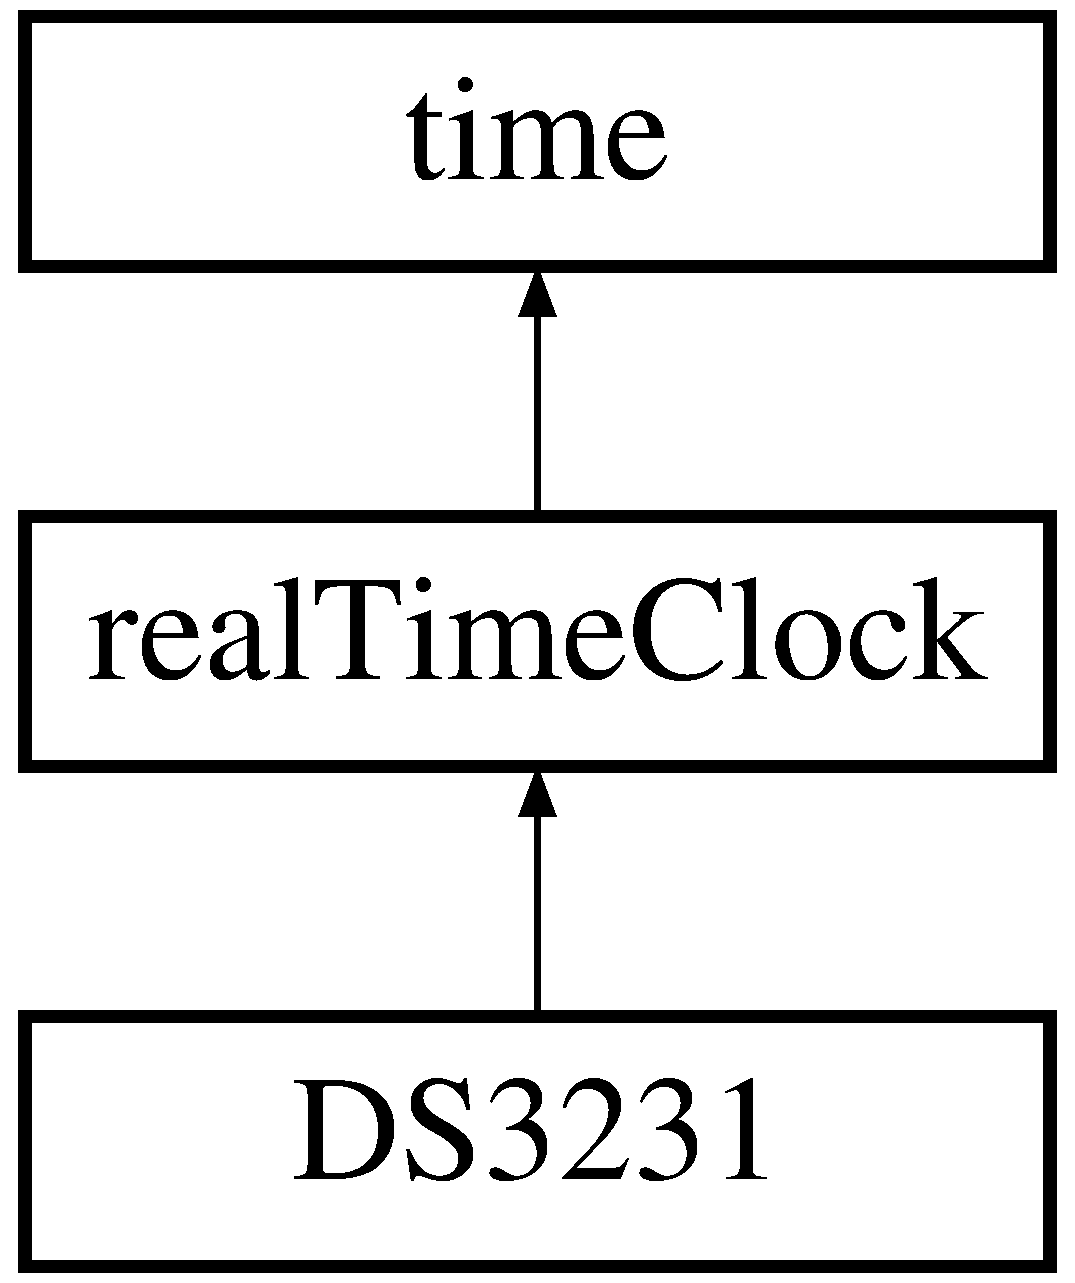
\includegraphics[height=3.000000cm]{class_d_s3231}
\end{center}
\end{figure}
\subsection*{Public Member Functions}
\begin{DoxyCompactItemize}
\item 
\mbox{\Hypertarget{class_d_s3231_a316537e9a09ce7ef57c1955785f1fa24}\label{class_d_s3231_a316537e9a09ce7ef57c1955785f1fa24}} 
{\bfseries D\+S3231} (\mbox{\hyperlink{classi2c_bus}{i2c\+Bus}} \&I2\+C\+Bus, uint8\+\_\+t address=default\+D\+S3231\+Address)
\item 
\mbox{\Hypertarget{class_d_s3231_a8a5357eae07991d94f8f7610a3f3073a}\label{class_d_s3231_a8a5357eae07991d94f8f7610a3f3073a}} 
uint8\+\_\+t {\bfseries get\+Current\+Seconds} () override
\item 
\mbox{\Hypertarget{class_d_s3231_ac73512cc6c2a37ffb21bee74ea835a09}\label{class_d_s3231_ac73512cc6c2a37ffb21bee74ea835a09}} 
void {\bfseries set\+Current\+Seconds} (uint8\+\_\+t new\+Seconds) override
\item 
\mbox{\Hypertarget{class_d_s3231_a08f384e1897214d4a201aaaecde3b8a4}\label{class_d_s3231_a08f384e1897214d4a201aaaecde3b8a4}} 
uint8\+\_\+t {\bfseries get\+Current\+Minutes} () override
\item 
\mbox{\Hypertarget{class_d_s3231_a221f92091b813108b3515f6676be29c8}\label{class_d_s3231_a221f92091b813108b3515f6676be29c8}} 
void {\bfseries set\+Current\+Minutes} (uint8\+\_\+t new\+Minutes) override
\item 
\mbox{\Hypertarget{class_d_s3231_a019d8ed8074a02937c0777424be3d0ae}\label{class_d_s3231_a019d8ed8074a02937c0777424be3d0ae}} 
uint8\+\_\+t {\bfseries get\+Current\+Hours} () override
\item 
\mbox{\Hypertarget{class_d_s3231_ae59c15abcccd8e27eadebcd150db810e}\label{class_d_s3231_ae59c15abcccd8e27eadebcd150db810e}} 
void {\bfseries set\+Current\+Hours} (uint8\+\_\+t new\+Hours) override
\item 
\mbox{\Hypertarget{class_d_s3231_a813bbe55a08e1911d498511795721477}\label{class_d_s3231_a813bbe55a08e1911d498511795721477}} 
uint8\+\_\+t {\bfseries get\+Current\+Day} () override
\item 
\mbox{\Hypertarget{class_d_s3231_ae43a887db6022008c066a257acd68ae8}\label{class_d_s3231_ae43a887db6022008c066a257acd68ae8}} 
void {\bfseries set\+Current\+Day} (uint8\+\_\+t new\+Day) override
\item 
\mbox{\Hypertarget{class_d_s3231_a346341a4d3c6615103b33fbff7a12884}\label{class_d_s3231_a346341a4d3c6615103b33fbff7a12884}} 
uint8\+\_\+t {\bfseries get\+Current\+Date} () override
\item 
\mbox{\Hypertarget{class_d_s3231_a597a0d5cb33f8b60f81dba9050ca1363}\label{class_d_s3231_a597a0d5cb33f8b60f81dba9050ca1363}} 
void {\bfseries set\+Current\+Date} (uint8\+\_\+t new\+Date) override
\item 
\mbox{\Hypertarget{class_d_s3231_a8d7a965802afacc16b4d5af86e0ed11e}\label{class_d_s3231_a8d7a965802afacc16b4d5af86e0ed11e}} 
uint8\+\_\+t {\bfseries get\+Current\+Month} () override
\item 
\mbox{\Hypertarget{class_d_s3231_a122611bf693cdd538178b99b893a7115}\label{class_d_s3231_a122611bf693cdd538178b99b893a7115}} 
void {\bfseries set\+Current\+Month} (uint8\+\_\+t new\+Month) override
\item 
\mbox{\Hypertarget{class_d_s3231_a38dfc1567d3419d5aeecd2062d4121c7}\label{class_d_s3231_a38dfc1567d3419d5aeecd2062d4121c7}} 
bool {\bfseries get\+Current\+Century\+Bit} () override
\item 
\mbox{\Hypertarget{class_d_s3231_a6477bd1bb91d3df6a088c369692f46a3}\label{class_d_s3231_a6477bd1bb91d3df6a088c369692f46a3}} 
void {\bfseries Reset\+Curent\+Century\+Bit} () override
\item 
\mbox{\Hypertarget{class_d_s3231_a28a340b10b045ad1e8b94532a57c3759}\label{class_d_s3231_a28a340b10b045ad1e8b94532a57c3759}} 
uint8\+\_\+t {\bfseries get\+Current\+Year} () override
\item 
\mbox{\Hypertarget{class_d_s3231_a59a60a725581bc8e5dcf857ea52c6281}\label{class_d_s3231_a59a60a725581bc8e5dcf857ea52c6281}} 
void {\bfseries set\+Current\+Year} (uint8\+\_\+t new\+Year) override
\item 
\mbox{\Hypertarget{class_d_s3231_abd46c1cf5f5c78e3222c3677e70a1272}\label{class_d_s3231_abd46c1cf5f5c78e3222c3677e70a1272}} 
int16\+\_\+t {\bfseries get\+Current\+Temperature\+Celsius} () override
\item 
\mbox{\Hypertarget{class_d_s3231_aa31acb133cc63aa7a2a25eda6244c9df}\label{class_d_s3231_aa31acb133cc63aa7a2a25eda6244c9df}} 
int16\+\_\+t {\bfseries get\+Current\+Temperature\+Fahrenheit} () override
\item 
\mbox{\Hypertarget{class_d_s3231_a0ca41c2242367c5ff1424d1b12f909c5}\label{class_d_s3231_a0ca41c2242367c5ff1424d1b12f909c5}} 
void {\bfseries get\+Current\+Time\+Data} (uint8\+\_\+t data\mbox{[}7\mbox{]}) override
\item 
\mbox{\Hypertarget{class_d_s3231_a04e087a918d2d48b0cdd2e3c6c2f595f}\label{class_d_s3231_a04e087a918d2d48b0cdd2e3c6c2f595f}} 
\mbox{\hyperlink{classtimestamp}{timestamp}} {\bfseries get\+Current\+Timestamp} () override
\item 
\mbox{\Hypertarget{class_d_s3231_ad94d54ed265fb5b911b4281f0103b0b0}\label{class_d_s3231_ad94d54ed265fb5b911b4281f0103b0b0}} 
void {\bfseries get\+Current\+Timestamp} (\mbox{\hyperlink{classtimestamp}{timestamp}} \&ts) override
\item 
\mbox{\Hypertarget{class_d_s3231_afd2b16482de8abc10981fdfca0e181a6}\label{class_d_s3231_afd2b16482de8abc10981fdfca0e181a6}} 
uint8\+\_\+t {\bfseries get\+Alarm\+One\+Seconds} () override
\item 
\mbox{\Hypertarget{class_d_s3231_ae294f3c8c8634a058846cf9864ccc5c8}\label{class_d_s3231_ae294f3c8c8634a058846cf9864ccc5c8}} 
void {\bfseries set\+Alarm\+One\+Seconds} (uint8\+\_\+t new\+Seconds) override
\item 
\mbox{\Hypertarget{class_d_s3231_ae11a0dcc34e9c8a9b875989172339957}\label{class_d_s3231_ae11a0dcc34e9c8a9b875989172339957}} 
uint8\+\_\+t {\bfseries get\+Alarm\+Minutes} (bool \mbox{\hyperlink{classalarm}{alarm}}) override
\item 
\mbox{\Hypertarget{class_d_s3231_a9c1f5b183c24f3062c1c8c299f46023c}\label{class_d_s3231_a9c1f5b183c24f3062c1c8c299f46023c}} 
void {\bfseries set\+Alarm\+Minutes} (bool \mbox{\hyperlink{classalarm}{alarm}}, uint8\+\_\+t new\+Minutes) override
\item 
\mbox{\Hypertarget{class_d_s3231_a8dc2f4546600209d16f109764c2f4434}\label{class_d_s3231_a8dc2f4546600209d16f109764c2f4434}} 
uint8\+\_\+t {\bfseries get\+Alarm\+Hours} (bool \mbox{\hyperlink{classalarm}{alarm}}) override
\item 
\mbox{\Hypertarget{class_d_s3231_a0bcc7e2285869ffbe29d19c593f5a447}\label{class_d_s3231_a0bcc7e2285869ffbe29d19c593f5a447}} 
void {\bfseries set\+Alarm\+Hours} (bool \mbox{\hyperlink{classalarm}{alarm}}, uint8\+\_\+t new\+Hours) override
\item 
\mbox{\Hypertarget{class_d_s3231_a0b013c68f96b5145c1c9feb9270855a7}\label{class_d_s3231_a0b013c68f96b5145c1c9feb9270855a7}} 
uint8\+\_\+t {\bfseries get\+Alarm\+Day\+Date} (bool \mbox{\hyperlink{classalarm}{alarm}}) override
\item 
\mbox{\Hypertarget{class_d_s3231_aa2048cc766ca58f707e84cbc564c1276}\label{class_d_s3231_aa2048cc766ca58f707e84cbc564c1276}} 
void {\bfseries set\+Alarm\+Day\+Date} (bool \mbox{\hyperlink{classalarm}{alarm}}, uint8\+\_\+t new\+Day\+Date) override
\item 
\mbox{\Hypertarget{class_d_s3231_a2e023e091c63208290e275874552a716}\label{class_d_s3231_a2e023e091c63208290e275874552a716}} 
uint8\+\_\+t {\bfseries get\+Control\+Register} () override
\item 
\mbox{\Hypertarget{class_d_s3231_a1151a22a8dd47470b22562cedae114e9}\label{class_d_s3231_a1151a22a8dd47470b22562cedae114e9}} 
void {\bfseries set\+Control\+Register} (uint8\+\_\+t new\+Byte) override
\item 
\mbox{\Hypertarget{class_d_s3231_a5b22edafc0d475fd6e33936c286654d5}\label{class_d_s3231_a5b22edafc0d475fd6e33936c286654d5}} 
bool {\bfseries get\+Control\+Register\+Bit} (uint8\+\_\+t bit\+Number) override
\item 
\mbox{\Hypertarget{class_d_s3231_a9ed1255adb58ecd03a541a4d481496c4}\label{class_d_s3231_a9ed1255adb58ecd03a541a4d481496c4}} 
void {\bfseries set\+Control\+Register\+Bit} (uint8\+\_\+t bit\+Number, bool new\+Bit) override
\item 
\mbox{\Hypertarget{class_d_s3231_aee77c6ecb3c292d375eebe7e58ebb024}\label{class_d_s3231_aee77c6ecb3c292d375eebe7e58ebb024}} 
uint8\+\_\+t {\bfseries get\+Status\+Register} () override
\item 
\mbox{\Hypertarget{class_d_s3231_a303a9a5123f66987e209396d60e329e8}\label{class_d_s3231_a303a9a5123f66987e209396d60e329e8}} 
void {\bfseries set\+Status\+Register} (uint8\+\_\+t new\+Byte) override
\item 
\mbox{\Hypertarget{class_d_s3231_a94e9f40f1b453dc4d8894b63bc0ec7d6}\label{class_d_s3231_a94e9f40f1b453dc4d8894b63bc0ec7d6}} 
int8\+\_\+t {\bfseries get\+Aging\+Offset} () override
\item 
\mbox{\Hypertarget{class_d_s3231_a0a9dc2668139654b261c2feeb1d6e663}\label{class_d_s3231_a0a9dc2668139654b261c2feeb1d6e663}} 
void {\bfseries set\+Aging\+Offset} (int8\+\_\+t new\+Aging\+Offset) override
\item 
\mbox{\Hypertarget{class_d_s3231_a143ec57122d892ea0ec671a153352f2c}\label{class_d_s3231_a143ec57122d892ea0ec671a153352f2c}} 
void {\bfseries update} () override
\end{DoxyCompactItemize}
\subsection*{Public Attributes}
\begin{DoxyCompactItemize}
\item 
\mbox{\Hypertarget{class_d_s3231_a46147c0e9191b205d02b141e497764fd}\label{class_d_s3231_a46147c0e9191b205d02b141e497764fd}} 
const uint8\+\_\+t {\bfseries B\+I\+T\+\_\+\+C\+O\+N\+T\+R\+O\+L\+\_\+\+A\+L\+A\+R\+M\+\_\+1\+\_\+\+I\+N\+T\+E\+R\+R\+U\+P\+T\+\_\+\+E\+N\+A\+B\+LE} = 0
\item 
\mbox{\Hypertarget{class_d_s3231_adc0c58cb34faa682a39d285613b41840}\label{class_d_s3231_adc0c58cb34faa682a39d285613b41840}} 
const uint8\+\_\+t {\bfseries B\+I\+T\+\_\+\+C\+O\+N\+T\+R\+O\+L\+\_\+\+A\+L\+A\+R\+M\+\_\+2\+\_\+\+I\+N\+T\+E\+R\+R\+U\+P\+T\+\_\+\+E\+N\+A\+B\+LE} = 1
\item 
\mbox{\Hypertarget{class_d_s3231_a60ae50496dfc48ea9d6d4f3be5a270e2}\label{class_d_s3231_a60ae50496dfc48ea9d6d4f3be5a270e2}} 
const uint8\+\_\+t {\bfseries B\+I\+T\+\_\+\+C\+O\+N\+T\+R\+O\+L\+\_\+\+I\+N\+T\+E\+R\+R\+U\+P\+T\+\_\+\+C\+O\+N\+T\+R\+OL} = 2
\item 
\mbox{\Hypertarget{class_d_s3231_aa59a7e767267dcdfd9d3769e65b448e9}\label{class_d_s3231_aa59a7e767267dcdfd9d3769e65b448e9}} 
const uint8\+\_\+t {\bfseries B\+I\+T\+\_\+\+C\+O\+N\+T\+O\+L\+\_\+\+R\+A\+T\+E\+\_\+\+S\+E\+L\+E\+C\+T\+\_\+1} = 3
\item 
\mbox{\Hypertarget{class_d_s3231_aeffda7b70a42c5c0010ab9736f24792e}\label{class_d_s3231_aeffda7b70a42c5c0010ab9736f24792e}} 
const uint8\+\_\+t {\bfseries B\+I\+T\+\_\+\+C\+O\+N\+T\+R\+O\+L\+\_\+\+R\+A\+T\+E\+\_\+\+S\+E\+L\+E\+C\+T\+\_\+2} = 4
\item 
\mbox{\Hypertarget{class_d_s3231_af7649567479c112648063a9a299ca9a9}\label{class_d_s3231_af7649567479c112648063a9a299ca9a9}} 
const uint8\+\_\+t {\bfseries B\+I\+T\+\_\+\+C\+O\+N\+T\+R\+O\+L\+\_\+\+T\+E\+M\+P\+E\+R\+A\+T\+U\+R\+E\+\_\+\+C\+O\+N\+V\+E\+RT} = 5
\item 
\mbox{\Hypertarget{class_d_s3231_a61f60873545487964d4b790fd5300f38}\label{class_d_s3231_a61f60873545487964d4b790fd5300f38}} 
const uint8\+\_\+t {\bfseries B\+I\+T\+\_\+\+C\+O\+N\+T\+R\+O\+L\+\_\+\+B\+A\+T\+T\+E\+R\+Y\+\_\+\+B\+A\+C\+K\+E\+D\+\_\+\+S\+QW} = 6
\item 
\mbox{\Hypertarget{class_d_s3231_aa65496ef80d4dc0a91c9c3386068593f}\label{class_d_s3231_aa65496ef80d4dc0a91c9c3386068593f}} 
const uint8\+\_\+t {\bfseries B\+I\+T\+\_\+\+C\+O\+N\+T\+R\+O\+L\+\_\+\+O\+S\+C\+I\+L\+L\+A\+T\+OR} = 7
\end{DoxyCompactItemize}
\subsection*{Private Member Functions}
\begin{DoxyCompactItemize}
\item 
\mbox{\Hypertarget{class_d_s3231_ae6ef1547a0d2c2653ae3fe4c0f6a62ff}\label{class_d_s3231_ae6ef1547a0d2c2653ae3fe4c0f6a62ff}} 
void {\bfseries set\+I2\+C\+Bus\+Current\+Address} ()
\item 
\mbox{\Hypertarget{class_d_s3231_a70033a61ca1965fa0aed9af31679355f}\label{class_d_s3231_a70033a61ca1965fa0aed9af31679355f}} 
uint8\+\_\+t {\bfseries get\+Alarm\+B\+C\+D\+Register\+Ex\+M\+SB} (uint8\+\_\+t alarm\+Register)
\item 
\mbox{\Hypertarget{class_d_s3231_a79280f7161eaa45b50fe649eda9c480a}\label{class_d_s3231_a79280f7161eaa45b50fe649eda9c480a}} 
void {\bfseries set\+Alarm\+B\+C\+D\+Register\+Ex\+M\+SB} (uint8\+\_\+t alarm\+Register, uint8\+\_\+t new\+Byte)
\end{DoxyCompactItemize}
\subsection*{Private Attributes}
\begin{DoxyCompactItemize}
\item 
\mbox{\Hypertarget{class_d_s3231_acffbcfc655349fd392b97dff5f18a56f}\label{class_d_s3231_acffbcfc655349fd392b97dff5f18a56f}} 
\mbox{\hyperlink{classi2c_bus}{i2c\+Bus}} \& {\bfseries I2\+C\+Bus}
\item 
\mbox{\Hypertarget{class_d_s3231_a905b445bb664b52529b3acbccbbaccb3}\label{class_d_s3231_a905b445bb664b52529b3acbccbbaccb3}} 
uint8\+\_\+t {\bfseries D\+S3231\+Address}
\item 
\mbox{\Hypertarget{class_d_s3231_a15fb987b624cdddde40a15db36665221}\label{class_d_s3231_a15fb987b624cdddde40a15db36665221}} 
int {\bfseries new\+Century}
\item 
\mbox{\Hypertarget{class_d_s3231_aaede356dfbcd2f22e8ac4103e67d4f8e}\label{class_d_s3231_aaede356dfbcd2f22e8ac4103e67d4f8e}} 
const uint8\+\_\+t {\bfseries R\+E\+G\+\_\+\+S\+E\+C\+O\+N\+DS} = 0x00
\item 
\mbox{\Hypertarget{class_d_s3231_affe134ab59f11a0fe7243f1172466fc2}\label{class_d_s3231_affe134ab59f11a0fe7243f1172466fc2}} 
const uint8\+\_\+t {\bfseries R\+E\+G\+\_\+\+M\+I\+N\+U\+T\+ES} = 0x01
\item 
\mbox{\Hypertarget{class_d_s3231_a80f6664a64967b5383933d314b57c7bc}\label{class_d_s3231_a80f6664a64967b5383933d314b57c7bc}} 
const uint8\+\_\+t {\bfseries R\+E\+G\+\_\+\+H\+O\+U\+RS} = 0x02
\item 
\mbox{\Hypertarget{class_d_s3231_a7fc54a4d1b80a74b003b451ee8fa6eda}\label{class_d_s3231_a7fc54a4d1b80a74b003b451ee8fa6eda}} 
const uint8\+\_\+t {\bfseries R\+E\+G\+\_\+\+D\+AY} = 0x03
\item 
\mbox{\Hypertarget{class_d_s3231_ad51434b6ef3bbc02bb2ddb18c1b70f2b}\label{class_d_s3231_ad51434b6ef3bbc02bb2ddb18c1b70f2b}} 
const uint8\+\_\+t {\bfseries R\+E\+G\+\_\+\+D\+A\+TE} = 0x04
\item 
\mbox{\Hypertarget{class_d_s3231_a20ac9f897ca08f0968c24c9a66703159}\label{class_d_s3231_a20ac9f897ca08f0968c24c9a66703159}} 
const uint8\+\_\+t {\bfseries R\+E\+G\+\_\+\+M\+O\+N\+T\+H\+\_\+\+C\+E\+N\+T\+U\+RY} = 0x05
\item 
\mbox{\Hypertarget{class_d_s3231_ada659ad8327043d2dc7e92988a943c03}\label{class_d_s3231_ada659ad8327043d2dc7e92988a943c03}} 
const uint8\+\_\+t {\bfseries R\+E\+G\+\_\+\+Y\+E\+AR} = 0x06
\item 
\mbox{\Hypertarget{class_d_s3231_a90aab5b318631c1d5bfb38ebcee822ac}\label{class_d_s3231_a90aab5b318631c1d5bfb38ebcee822ac}} 
const uint8\+\_\+t {\bfseries R\+E\+G\+\_\+\+A\+L\+A\+R\+M\+\_\+1\+\_\+\+S\+EC} = 0x07
\item 
\mbox{\Hypertarget{class_d_s3231_a31ea11d7f117cd181868b76c7580ff9a}\label{class_d_s3231_a31ea11d7f117cd181868b76c7580ff9a}} 
const uint8\+\_\+t {\bfseries R\+E\+G\+\_\+\+A\+L\+A\+R\+M\+\_\+1\+\_\+\+M\+IN} = 0x08
\item 
\mbox{\Hypertarget{class_d_s3231_a38f8b765f3a23dcf6e1e402b6b4955a4}\label{class_d_s3231_a38f8b765f3a23dcf6e1e402b6b4955a4}} 
const uint8\+\_\+t {\bfseries R\+E\+G\+\_\+\+A\+L\+A\+R\+M\+\_\+1\+\_\+\+H\+O\+U\+RS} = 0x09
\item 
\mbox{\Hypertarget{class_d_s3231_ae16ac34f6a6d25ec7709745b1671a34c}\label{class_d_s3231_ae16ac34f6a6d25ec7709745b1671a34c}} 
const uint8\+\_\+t {\bfseries R\+E\+G\+\_\+\+A\+L\+A\+R\+M\+\_\+1\+\_\+\+D\+A\+Y\+\_\+\+D\+A\+TE} = 0x0A
\item 
\mbox{\Hypertarget{class_d_s3231_aca2b9311735fff7dded9877d48e8284d}\label{class_d_s3231_aca2b9311735fff7dded9877d48e8284d}} 
const uint8\+\_\+t {\bfseries R\+E\+G\+\_\+\+A\+L\+A\+R\+M\+\_\+2\+\_\+\+M\+IN} = 0x0B
\item 
\mbox{\Hypertarget{class_d_s3231_ac8f2d234a9e303fe71b52a32a3571d7d}\label{class_d_s3231_ac8f2d234a9e303fe71b52a32a3571d7d}} 
const uint8\+\_\+t {\bfseries R\+E\+G\+\_\+\+A\+L\+A\+R\+M\+\_\+2\+\_\+\+H\+O\+U\+RS} = 0x0C
\item 
\mbox{\Hypertarget{class_d_s3231_a05deee6f4c941a37c95f773cc7a369a3}\label{class_d_s3231_a05deee6f4c941a37c95f773cc7a369a3}} 
const uint8\+\_\+t {\bfseries R\+E\+G\+\_\+\+A\+L\+A\+R\+M\+\_\+2\+\_\+\+D\+A\+Y\+\_\+\+D\+A\+TE} = 0x0D
\item 
\mbox{\Hypertarget{class_d_s3231_adc5a414930fd2cf9038dd3096ed4da1f}\label{class_d_s3231_adc5a414930fd2cf9038dd3096ed4da1f}} 
const uint8\+\_\+t {\bfseries R\+E\+G\+\_\+\+C\+O\+N\+T\+R\+OL} = 0x0E
\item 
\mbox{\Hypertarget{class_d_s3231_a242154f8eff5f7005d47c394b02251de}\label{class_d_s3231_a242154f8eff5f7005d47c394b02251de}} 
const uint8\+\_\+t {\bfseries R\+E\+G\+\_\+\+S\+T\+A\+T\+US} = 0x0F
\item 
\mbox{\Hypertarget{class_d_s3231_a8a48b6c5dc799fce792806d8307a869e}\label{class_d_s3231_a8a48b6c5dc799fce792806d8307a869e}} 
const uint8\+\_\+t {\bfseries R\+E\+G\+\_\+\+A\+G\+I\+N\+G\+\_\+\+O\+F\+F\+S\+ET} = 0x10
\item 
\mbox{\Hypertarget{class_d_s3231_a0334c3d383e5f28df368f21062672228}\label{class_d_s3231_a0334c3d383e5f28df368f21062672228}} 
const uint8\+\_\+t {\bfseries R\+E\+G\+\_\+\+T\+E\+M\+P\+E\+R\+A\+T\+U\+R\+E\+\_\+\+M\+SB} = 0x11
\item 
\mbox{\Hypertarget{class_d_s3231_a6bc742bfa52c83f252787045c9952a45}\label{class_d_s3231_a6bc742bfa52c83f252787045c9952a45}} 
const uint8\+\_\+t {\bfseries R\+E\+G\+\_\+\+T\+E\+M\+P\+E\+R\+A\+T\+U\+R\+E\+\_\+\+L\+SB} = 0x12
\item 
\mbox{\Hypertarget{class_d_s3231_a5f55646a365acc7123c76b2c363eb416}\label{class_d_s3231_a5f55646a365acc7123c76b2c363eb416}} 
const uint8\+\_\+t {\bfseries B\+I\+T\+\_\+\+A\+L\+A\+R\+M\+\_\+\+Ax\+Mx} = 7
\end{DoxyCompactItemize}
\subsection*{Static Private Attributes}
\begin{DoxyCompactItemize}
\item 
\mbox{\Hypertarget{class_d_s3231_a9c6b5e3dea008155e78dfc6623fe41b9}\label{class_d_s3231_a9c6b5e3dea008155e78dfc6623fe41b9}} 
static const uint8\+\_\+t {\bfseries default\+D\+S3231\+Address} = 0x68
\end{DoxyCompactItemize}
\subsection*{Additional Inherited Members}


The documentation for this class was generated from the following files\+:\begin{DoxyCompactItemize}
\item 
Demo/D\+S3231.\+hpp\item 
Demo/D\+S3231.\+cpp\end{DoxyCompactItemize}

\hypertarget{class_h_c_s_r501}{}\section{H\+C\+S\+R501 Class Reference}
\label{class_h_c_s_r501}\index{H\+C\+S\+R501@{H\+C\+S\+R501}}
Inheritance diagram for H\+C\+S\+R501\+:\begin{figure}[H]
\begin{center}
\leavevmode
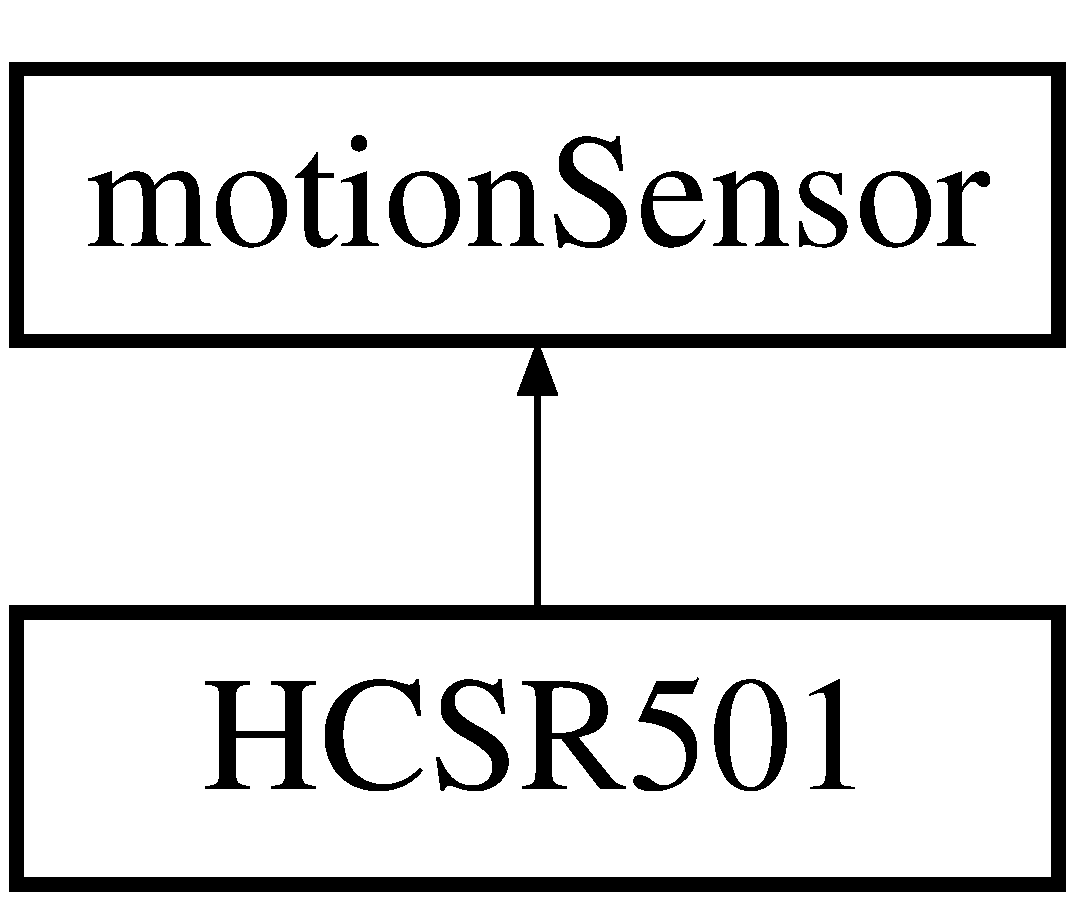
\includegraphics[height=2.000000cm]{class_h_c_s_r501}
\end{center}
\end{figure}
\subsection*{Public Member Functions}
\begin{DoxyCompactItemize}
\item 
\mbox{\Hypertarget{class_h_c_s_r501_a589a13daf993e217138344db60086f36}\label{class_h_c_s_r501_a589a13daf993e217138344db60086f36}} 
{\bfseries H\+C\+S\+R501} (hwlib\+::pin\+\_\+in \&input)
\item 
\mbox{\Hypertarget{class_h_c_s_r501_a75456a573bf0066ee648f8f1a39d4966}\label{class_h_c_s_r501_a75456a573bf0066ee648f8f1a39d4966}} 
bool {\bfseries detect} () override
\end{DoxyCompactItemize}
\subsection*{Private Attributes}
\begin{DoxyCompactItemize}
\item 
\mbox{\Hypertarget{class_h_c_s_r501_a00d41bcf68fa634e07ae68488d2b61ee}\label{class_h_c_s_r501_a00d41bcf68fa634e07ae68488d2b61ee}} 
hwlib\+::pin\+\_\+in \& {\bfseries input}
\end{DoxyCompactItemize}


The documentation for this class was generated from the following files\+:\begin{DoxyCompactItemize}
\item 
Demo/H\+C\+S\+R501.\+hpp\item 
Demo/H\+C\+S\+R501.\+cpp\end{DoxyCompactItemize}

\hypertarget{classi2c_bus}{}\section{i2c\+Bus Class Reference}
\label{classi2c_bus}\index{i2c\+Bus@{i2c\+Bus}}


Basic I2C functions like write and read a register.  




{\ttfamily \#include $<$i2c\+Bus.\+hpp$>$}

Inheritance diagram for i2c\+Bus\+:\begin{figure}[H]
\begin{center}
\leavevmode
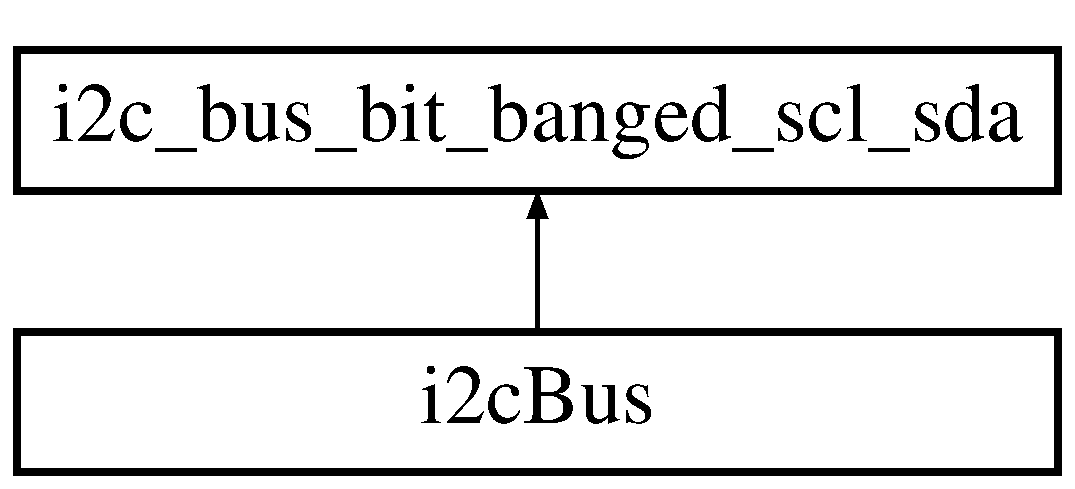
\includegraphics[height=2.000000cm]{classi2c_bus}
\end{center}
\end{figure}
\subsection*{Public Member Functions}
\begin{DoxyCompactItemize}
\item 
\mbox{\hyperlink{classi2c_bus_aa2f1a1a391410e33dc4f09c6f5b9ae7c}{i2c\+Bus}} (hwlib\+::pin\+\_\+oc \&scl, hwlib\+::pin\+\_\+oc \&sda)
\begin{DoxyCompactList}\small\item\em Constructor for the \mbox{\hyperlink{classi2c_bus}{i2c\+Bus}}. \end{DoxyCompactList}\item 
void \mbox{\hyperlink{classi2c_bus_a5f3a99851f437473a00f1216ba2a1517}{set\+Current\+Chip\+Address}} (uint8\+\_\+t new\+Chip\+Address)
\begin{DoxyCompactList}\small\item\em Set \mbox{\hyperlink{classi2c_bus_a64ff87527c88619d72ede947d73eac3a}{current\+Chip\+Address}} to another address. \end{DoxyCompactList}\item 
uint8\+\_\+t \mbox{\hyperlink{classi2c_bus_aba70817c7bc0a9ad73b369616a864395}{get\+Current\+Chip\+Address}} ()
\begin{DoxyCompactList}\small\item\em Returns the value of the current chip you are communicating with. \end{DoxyCompactList}\item 
void \mbox{\hyperlink{classi2c_bus_adee2545c8b692474b6814b4605e48ec3}{set\+Register}} (uint8\+\_\+t chip\+Reg\+Address)
\begin{DoxyCompactList}\small\item\em set the interal register pointer of \mbox{\hyperlink{classi2c_bus_a64ff87527c88619d72ede947d73eac3a}{current\+Chip\+Address}}. \end{DoxyCompactList}\item 
uint8\+\_\+t \mbox{\hyperlink{classi2c_bus_a7f83afc0264e758214db63cca336846d}{get\+Byte\+From\+Register}} (uint8\+\_\+t chip\+Reg\+Address)
\begin{DoxyCompactList}\small\item\em Get byte from a specific register address. \end{DoxyCompactList}\item 
uint8\+\_\+t \mbox{\hyperlink{classi2c_bus_a30d44d89d2f9b0d290cb2a207f6a4777}{get\+D\+E\+C\+From\+B\+C\+D\+Register}} (uint8\+\_\+t chip\+Reg\+Address)
\begin{DoxyCompactList}\small\item\em Get a decimal value from a register containing B\+CD value. \end{DoxyCompactList}\item 
void \mbox{\hyperlink{classi2c_bus_a8bed9bf37dee74b691ab4c92723dd206}{set\+Byte\+In\+Register}} (uint8\+\_\+t chip\+Reg\+Address, uint8\+\_\+t byte)
\begin{DoxyCompactList}\small\item\em Set byte into a specific register address. \end{DoxyCompactList}\item 
void \mbox{\hyperlink{classi2c_bus_a31c36069cff15f73aa54703a6ee8b951}{set\+Byte\+To\+B\+C\+D\+In\+Register}} (uint8\+\_\+t chip\+Reg\+Address, uint8\+\_\+t byte)
\begin{DoxyCompactList}\small\item\em set a decimal value into a register containing B\+CD value. \end{DoxyCompactList}\item 
bool \mbox{\hyperlink{classi2c_bus_aeedd7fa6ab6640fe86bcfb8a3ac3f306}{get\+Bit\+From\+Register}} (uint8\+\_\+t chip\+Reg\+Address, uint8\+\_\+t bit\+Number)
\begin{DoxyCompactList}\small\item\em Get bit from a specific register address. \end{DoxyCompactList}\item 
void \mbox{\hyperlink{classi2c_bus_a3b2f595372a05bde8e1cf9d6a86f2bdb}{set\+Bit\+In\+Register}} (uint8\+\_\+t chip\+Reg\+Address, uint8\+\_\+t bit\+Number)
\begin{DoxyCompactList}\small\item\em Set bit into a specific register address (This function will always set the bit to H\+I\+G\+H/1). \end{DoxyCompactList}\item 
void \mbox{\hyperlink{classi2c_bus_a30c140f08712618bc46f7c98ba1da3c3}{clear\+Bit\+In\+Register}} (uint8\+\_\+t chip\+Reg\+Address, uint8\+\_\+t bit\+Number)
\begin{DoxyCompactList}\small\item\em Clear bit of specific register address (This function will always set the bit to L\+O\+W/0). \end{DoxyCompactList}\end{DoxyCompactItemize}
\subsection*{Private Attributes}
\begin{DoxyCompactItemize}
\item 
uint8\+\_\+t \mbox{\hyperlink{classi2c_bus_a64ff87527c88619d72ede947d73eac3a}{current\+Chip\+Address}} = 0x00
\begin{DoxyCompactList}\small\item\em This variable stores the address of the chip you want to talk with. \end{DoxyCompactList}\end{DoxyCompactItemize}


\subsection{Detailed Description}
Basic I2C functions like write and read a register. 

This class is a wrapper around the hwlib\+::i2c\+\_\+bus\+\_\+bit\+\_\+banged\+\_\+scl\+\_\+sda (\href{mailto:wouter@voti.nl}{\tt wouter@voti.\+nl} 2017). It contains some basic I2C functions for easy access of the used module. \begin{DoxyWarning}{Warning}
T\+HE S\+O\+F\+T\+W\+A\+RE IS P\+R\+O\+V\+I\+D\+ED \char`\"{}\+A\+S I\+S\char`\"{}, W\+I\+T\+H\+O\+UT W\+A\+R\+R\+A\+N\+TY OF A\+NY K\+I\+ND. 
\end{DoxyWarning}


\subsection{Constructor \& Destructor Documentation}
\mbox{\Hypertarget{classi2c_bus_aa2f1a1a391410e33dc4f09c6f5b9ae7c}\label{classi2c_bus_aa2f1a1a391410e33dc4f09c6f5b9ae7c}} 
\index{i2c\+Bus@{i2c\+Bus}!i2c\+Bus@{i2c\+Bus}}
\index{i2c\+Bus@{i2c\+Bus}!i2c\+Bus@{i2c\+Bus}}
\subsubsection{\texorpdfstring{i2c\+Bus()}{i2cBus()}}
{\footnotesize\ttfamily i2c\+Bus\+::i2c\+Bus (\begin{DoxyParamCaption}\item[{hwlib\+::pin\+\_\+oc \&}]{scl,  }\item[{hwlib\+::pin\+\_\+oc \&}]{sda }\end{DoxyParamCaption})}



Constructor for the \mbox{\hyperlink{classi2c_bus}{i2c\+Bus}}. 


\begin{DoxyParams}{Parameters}
{\em scl} & Serial clock line. \\
\hline
{\em sda} & Serial Data line. \\
\hline
\end{DoxyParams}


\subsection{Member Function Documentation}
\mbox{\Hypertarget{classi2c_bus_a30c140f08712618bc46f7c98ba1da3c3}\label{classi2c_bus_a30c140f08712618bc46f7c98ba1da3c3}} 
\index{i2c\+Bus@{i2c\+Bus}!clear\+Bit\+In\+Register@{clear\+Bit\+In\+Register}}
\index{clear\+Bit\+In\+Register@{clear\+Bit\+In\+Register}!i2c\+Bus@{i2c\+Bus}}
\subsubsection{\texorpdfstring{clear\+Bit\+In\+Register()}{clearBitInRegister()}}
{\footnotesize\ttfamily void i2c\+Bus\+::clear\+Bit\+In\+Register (\begin{DoxyParamCaption}\item[{uint8\+\_\+t}]{chip\+Reg\+Address,  }\item[{uint8\+\_\+t}]{bit\+Number }\end{DoxyParamCaption})}



Clear bit of specific register address (This function will always set the bit to L\+O\+W/0). 


\begin{DoxyParams}{Parameters}
{\em chip\+Reg\+Address} & the register address where you want to clear the bit. \\
\hline
{\em bit\+Number} & the bit you want to clear the value of (0 = L\+SB, 7 = M\+SB).\\
\hline
\end{DoxyParams}
First this function gets the current byte in the register. After achieving the whole byte it will clear the bit given by the user(bit\+Number). And last but not least it will set the manipulated byte into the register using \mbox{\hyperlink{classi2c_bus_a8bed9bf37dee74b691ab4c92723dd206}{set\+Byte\+In\+Register}} \begin{DoxyWarning}{Warning}
The value of the bit will be overridden. 
\end{DoxyWarning}
\mbox{\Hypertarget{classi2c_bus_aeedd7fa6ab6640fe86bcfb8a3ac3f306}\label{classi2c_bus_aeedd7fa6ab6640fe86bcfb8a3ac3f306}} 
\index{i2c\+Bus@{i2c\+Bus}!get\+Bit\+From\+Register@{get\+Bit\+From\+Register}}
\index{get\+Bit\+From\+Register@{get\+Bit\+From\+Register}!i2c\+Bus@{i2c\+Bus}}
\subsubsection{\texorpdfstring{get\+Bit\+From\+Register()}{getBitFromRegister()}}
{\footnotesize\ttfamily bool i2c\+Bus\+::get\+Bit\+From\+Register (\begin{DoxyParamCaption}\item[{uint8\+\_\+t}]{chip\+Reg\+Address,  }\item[{uint8\+\_\+t}]{bit\+Number }\end{DoxyParamCaption})}



Get bit from a specific register address. 


\begin{DoxyParams}{Parameters}
{\em chip\+Reg\+Address} & the register address you want the bit from. \\
\hline
{\em bit\+Number} & the bit you want to get from the register (0 = L\+SB, 7 = M\+SB). \\
\hline
\end{DoxyParams}
\begin{DoxyReturn}{Returns}
A boolean containing the the bit value of the give bit\+Number.
\end{DoxyReturn}
First it will get the whole byte using \mbox{\hyperlink{classi2c_bus_a7f83afc0264e758214db63cca336846d}{get\+Byte\+From\+Register}}. After achieving the whole byte it will bitshift to the right bit and return that specific bit. \mbox{\Hypertarget{classi2c_bus_a7f83afc0264e758214db63cca336846d}\label{classi2c_bus_a7f83afc0264e758214db63cca336846d}} 
\index{i2c\+Bus@{i2c\+Bus}!get\+Byte\+From\+Register@{get\+Byte\+From\+Register}}
\index{get\+Byte\+From\+Register@{get\+Byte\+From\+Register}!i2c\+Bus@{i2c\+Bus}}
\subsubsection{\texorpdfstring{get\+Byte\+From\+Register()}{getByteFromRegister()}}
{\footnotesize\ttfamily uint8\+\_\+t i2c\+Bus\+::get\+Byte\+From\+Register (\begin{DoxyParamCaption}\item[{uint8\+\_\+t}]{chip\+Reg\+Address }\end{DoxyParamCaption})}



Get byte from a specific register address. 


\begin{DoxyParams}{Parameters}
{\em chip\+Reg\+Address} & the register address you want the byte from. \\
\hline
\end{DoxyParams}
\begin{DoxyReturn}{Returns}
A uint8\+\_\+t containing the byte of the give chip\+Reg\+Address.
\end{DoxyReturn}
This method will only get one byte from the \mbox{\hyperlink{classi2c_bus_a64ff87527c88619d72ede947d73eac3a}{current\+Chip\+Address}} and returns it. First the internal register pointer is set using \mbox{\hyperlink{classi2c_bus_adee2545c8b692474b6814b4605e48ec3}{set\+Register}}. After that the byte is read using hwlib\+::i2c\+\_\+bus\+\_\+bit\+\_\+banged\+\_\+scl\+\_\+sda.\+read (\href{mailto:wouter@voti.nl}{\tt wouter@voti.\+nl} 2017). \mbox{\Hypertarget{classi2c_bus_aba70817c7bc0a9ad73b369616a864395}\label{classi2c_bus_aba70817c7bc0a9ad73b369616a864395}} 
\index{i2c\+Bus@{i2c\+Bus}!get\+Current\+Chip\+Address@{get\+Current\+Chip\+Address}}
\index{get\+Current\+Chip\+Address@{get\+Current\+Chip\+Address}!i2c\+Bus@{i2c\+Bus}}
\subsubsection{\texorpdfstring{get\+Current\+Chip\+Address()}{getCurrentChipAddress()}}
{\footnotesize\ttfamily uint8\+\_\+t i2c\+Bus\+::get\+Current\+Chip\+Address (\begin{DoxyParamCaption}{ }\end{DoxyParamCaption})}



Returns the value of the current chip you are communicating with. 

\begin{DoxyReturn}{Returns}
A uint8\+\_\+t containing the value of \mbox{\hyperlink{classi2c_bus_a64ff87527c88619d72ede947d73eac3a}{current\+Chip\+Address}}. 
\end{DoxyReturn}
\mbox{\Hypertarget{classi2c_bus_a30d44d89d2f9b0d290cb2a207f6a4777}\label{classi2c_bus_a30d44d89d2f9b0d290cb2a207f6a4777}} 
\index{i2c\+Bus@{i2c\+Bus}!get\+D\+E\+C\+From\+B\+C\+D\+Register@{get\+D\+E\+C\+From\+B\+C\+D\+Register}}
\index{get\+D\+E\+C\+From\+B\+C\+D\+Register@{get\+D\+E\+C\+From\+B\+C\+D\+Register}!i2c\+Bus@{i2c\+Bus}}
\subsubsection{\texorpdfstring{get\+D\+E\+C\+From\+B\+C\+D\+Register()}{getDECFromBCDRegister()}}
{\footnotesize\ttfamily uint8\+\_\+t i2c\+Bus\+::get\+D\+E\+C\+From\+B\+C\+D\+Register (\begin{DoxyParamCaption}\item[{uint8\+\_\+t}]{chip\+Reg\+Address }\end{DoxyParamCaption})}



Get a decimal value from a register containing B\+CD value. 


\begin{DoxyParams}{Parameters}
{\em chip\+Reg\+Address} & the register address you want the decimal value from. \\
\hline
\end{DoxyParams}
\begin{DoxyReturn}{Returns}
A uint8\+\_\+t containing the decimal value
\end{DoxyReturn}
This method gets the value of the register using \mbox{\hyperlink{classi2c_bus_a7f83afc0264e758214db63cca336846d}{get\+Byte\+From\+Register}}. After getting the byte it uses B\+C\+D\+To\+D\+E\+C() to turn the B\+C\+D-\/code into a decimal value. the B\+C\+D\+To\+D\+EC function is located in the following file\+: \mbox{\hyperlink{bit_parser_8hpp_source}{bit\+Parser.\+hpp}}. \mbox{\Hypertarget{classi2c_bus_a3b2f595372a05bde8e1cf9d6a86f2bdb}\label{classi2c_bus_a3b2f595372a05bde8e1cf9d6a86f2bdb}} 
\index{i2c\+Bus@{i2c\+Bus}!set\+Bit\+In\+Register@{set\+Bit\+In\+Register}}
\index{set\+Bit\+In\+Register@{set\+Bit\+In\+Register}!i2c\+Bus@{i2c\+Bus}}
\subsubsection{\texorpdfstring{set\+Bit\+In\+Register()}{setBitInRegister()}}
{\footnotesize\ttfamily void i2c\+Bus\+::set\+Bit\+In\+Register (\begin{DoxyParamCaption}\item[{uint8\+\_\+t}]{chip\+Reg\+Address,  }\item[{uint8\+\_\+t}]{bit\+Number }\end{DoxyParamCaption})}



Set bit into a specific register address (This function will always set the bit to H\+I\+G\+H/1). 


\begin{DoxyParams}{Parameters}
{\em chip\+Reg\+Address} & the register address where you want to set the bit. \\
\hline
{\em bit\+Number} & the bit you want to set the value of (0 = L\+SB, 7 = M\+SB).\\
\hline
\end{DoxyParams}
First this function gets the current byte in the register. After achieving the whole byte it will set the bit given by the user(bit\+Number). And last but not least it will set the manipulated byte into the register using \mbox{\hyperlink{classi2c_bus_a8bed9bf37dee74b691ab4c92723dd206}{set\+Byte\+In\+Register}} \begin{DoxyWarning}{Warning}
The value of the bit will be overridden. 
\end{DoxyWarning}
\mbox{\Hypertarget{classi2c_bus_a8bed9bf37dee74b691ab4c92723dd206}\label{classi2c_bus_a8bed9bf37dee74b691ab4c92723dd206}} 
\index{i2c\+Bus@{i2c\+Bus}!set\+Byte\+In\+Register@{set\+Byte\+In\+Register}}
\index{set\+Byte\+In\+Register@{set\+Byte\+In\+Register}!i2c\+Bus@{i2c\+Bus}}
\subsubsection{\texorpdfstring{set\+Byte\+In\+Register()}{setByteInRegister()}}
{\footnotesize\ttfamily void i2c\+Bus\+::set\+Byte\+In\+Register (\begin{DoxyParamCaption}\item[{uint8\+\_\+t}]{chip\+Reg\+Address,  }\item[{uint8\+\_\+t}]{byte }\end{DoxyParamCaption})}



Set byte into a specific register address. 


\begin{DoxyParams}{Parameters}
{\em chip\+Reg\+Address} & the register address you want to set the byte into. \\
\hline
{\em byte} & this is the byte you want te set into the register.\\
\hline
\end{DoxyParams}
This method will set a byte into the given register address(\#chip\+Reg\+Address). The chip it will be communicating with is specified by \mbox{\hyperlink{classi2c_bus_a64ff87527c88619d72ede947d73eac3a}{current\+Chip\+Address}}. First the internal register pointer is set using \mbox{\hyperlink{classi2c_bus_adee2545c8b692474b6814b4605e48ec3}{set\+Register}}. After that the byte is written using hwlib\+::i2c\+\_\+bus\+\_\+bit\+\_\+banged\+\_\+scl\+\_\+sda.\+write (\href{mailto:wouter@voti.nl}{\tt wouter@voti.\+nl} 2017). \begin{DoxyWarning}{Warning}
the value of the register will be overridden. 
\end{DoxyWarning}
\mbox{\Hypertarget{classi2c_bus_a31c36069cff15f73aa54703a6ee8b951}\label{classi2c_bus_a31c36069cff15f73aa54703a6ee8b951}} 
\index{i2c\+Bus@{i2c\+Bus}!set\+Byte\+To\+B\+C\+D\+In\+Register@{set\+Byte\+To\+B\+C\+D\+In\+Register}}
\index{set\+Byte\+To\+B\+C\+D\+In\+Register@{set\+Byte\+To\+B\+C\+D\+In\+Register}!i2c\+Bus@{i2c\+Bus}}
\subsubsection{\texorpdfstring{set\+Byte\+To\+B\+C\+D\+In\+Register()}{setByteToBCDInRegister()}}
{\footnotesize\ttfamily void i2c\+Bus\+::set\+Byte\+To\+B\+C\+D\+In\+Register (\begin{DoxyParamCaption}\item[{uint8\+\_\+t}]{chip\+Reg\+Address,  }\item[{uint8\+\_\+t}]{byte }\end{DoxyParamCaption})}



set a decimal value into a register containing B\+CD value. 


\begin{DoxyParams}{Parameters}
{\em chip\+Reg\+Address} & the register address you want to set the decimal value in. \\
\hline
{\em byte} & the decimal value(byte) you want to set into the register.\\
\hline
\end{DoxyParams}
This function turns the decimal byte into a B\+C\+D-\/coded value using the the function D\+E\+C\+To\+B\+CD which is located the following file\+: \mbox{\hyperlink{bit_parser_8hpp_source}{bit\+Parser.\+hpp}}. After turning the decimal value into a B\+C\+D-\/coded byte it sends the value using \mbox{\hyperlink{classi2c_bus_a8bed9bf37dee74b691ab4c92723dd206}{set\+Byte\+In\+Register}}. \begin{DoxyWarning}{Warning}
The value of the register will be overridden. 
\end{DoxyWarning}
\mbox{\Hypertarget{classi2c_bus_a5f3a99851f437473a00f1216ba2a1517}\label{classi2c_bus_a5f3a99851f437473a00f1216ba2a1517}} 
\index{i2c\+Bus@{i2c\+Bus}!set\+Current\+Chip\+Address@{set\+Current\+Chip\+Address}}
\index{set\+Current\+Chip\+Address@{set\+Current\+Chip\+Address}!i2c\+Bus@{i2c\+Bus}}
\subsubsection{\texorpdfstring{set\+Current\+Chip\+Address()}{setCurrentChipAddress()}}
{\footnotesize\ttfamily void i2c\+Bus\+::set\+Current\+Chip\+Address (\begin{DoxyParamCaption}\item[{uint8\+\_\+t}]{new\+Chip\+Address }\end{DoxyParamCaption})}



Set \mbox{\hyperlink{classi2c_bus_a64ff87527c88619d72ede947d73eac3a}{current\+Chip\+Address}} to another address. 


\begin{DoxyParams}{Parameters}
{\em new\+Chip\+Address} & This will be the new value of \mbox{\hyperlink{classi2c_bus_a64ff87527c88619d72ede947d73eac3a}{current\+Chip\+Address}}. \\
\hline
\end{DoxyParams}
\begin{DoxyWarning}{Warning}
Changing \mbox{\hyperlink{classi2c_bus_a64ff87527c88619d72ede947d73eac3a}{current\+Chip\+Address}} means that you will be communicating with another chip from now on. 
\end{DoxyWarning}
\mbox{\Hypertarget{classi2c_bus_adee2545c8b692474b6814b4605e48ec3}\label{classi2c_bus_adee2545c8b692474b6814b4605e48ec3}} 
\index{i2c\+Bus@{i2c\+Bus}!set\+Register@{set\+Register}}
\index{set\+Register@{set\+Register}!i2c\+Bus@{i2c\+Bus}}
\subsubsection{\texorpdfstring{set\+Register()}{setRegister()}}
{\footnotesize\ttfamily void i2c\+Bus\+::set\+Register (\begin{DoxyParamCaption}\item[{uint8\+\_\+t}]{chip\+Reg\+Address }\end{DoxyParamCaption})}



set the interal register pointer of \mbox{\hyperlink{classi2c_bus_a64ff87527c88619d72ede947d73eac3a}{current\+Chip\+Address}}. 


\begin{DoxyParams}{Parameters}
{\em chip\+Reg\+Address} & the register address you want the interal register pointer to set to.\\
\hline
\end{DoxyParams}
This function sends one byte in a array containing \#chip\+Reg\+Address. This array will be sent using hwlib\+::i2c\+\_\+bus\+\_\+bit\+\_\+banged\+\_\+scl\+\_\+sda.\+write (\href{mailto:wouter@voti.nl}{\tt wouter@voti.\+nl} 2017). \begin{DoxyWarning}{Warning}
the internal register pointer value will be overridden. 
\end{DoxyWarning}


\subsection{Member Data Documentation}
\mbox{\Hypertarget{classi2c_bus_a64ff87527c88619d72ede947d73eac3a}\label{classi2c_bus_a64ff87527c88619d72ede947d73eac3a}} 
\index{i2c\+Bus@{i2c\+Bus}!current\+Chip\+Address@{current\+Chip\+Address}}
\index{current\+Chip\+Address@{current\+Chip\+Address}!i2c\+Bus@{i2c\+Bus}}
\subsubsection{\texorpdfstring{current\+Chip\+Address}{currentChipAddress}}
{\footnotesize\ttfamily uint8\+\_\+t i2c\+Bus\+::current\+Chip\+Address = 0x00\hspace{0.3cm}{\ttfamily [private]}}



This variable stores the address of the chip you want to talk with. 

Every function that communicates with a chip will send this byte first to let all the chips know we want to communicate with the chip using this address. \begin{DoxyWarning}{Warning}
Changing \mbox{\hyperlink{classi2c_bus_a64ff87527c88619d72ede947d73eac3a}{current\+Chip\+Address}} means that you will be communicating with another chip from now on. 
\end{DoxyWarning}


The documentation for this class was generated from the following files\+:\begin{DoxyCompactItemize}
\item 
Demo/i2c\+Bus.\+hpp\item 
Demo/i2c\+Bus.\+cpp\end{DoxyCompactItemize}

\hypertarget{class_m_f_r_c522}{}\section{M\+F\+R\+C522 Class Reference}
\label{class_m_f_r_c522}\index{M\+F\+R\+C522@{M\+F\+R\+C522}}


This class is used to communicate with the \mbox{\hyperlink{class_m_f_r_c522}{M\+F\+R\+C522}} chip.  




{\ttfamily \#include $<$M\+F\+R\+C522.\+hpp$>$}

Inheritance diagram for M\+F\+R\+C522\+:\begin{figure}[H]
\begin{center}
\leavevmode
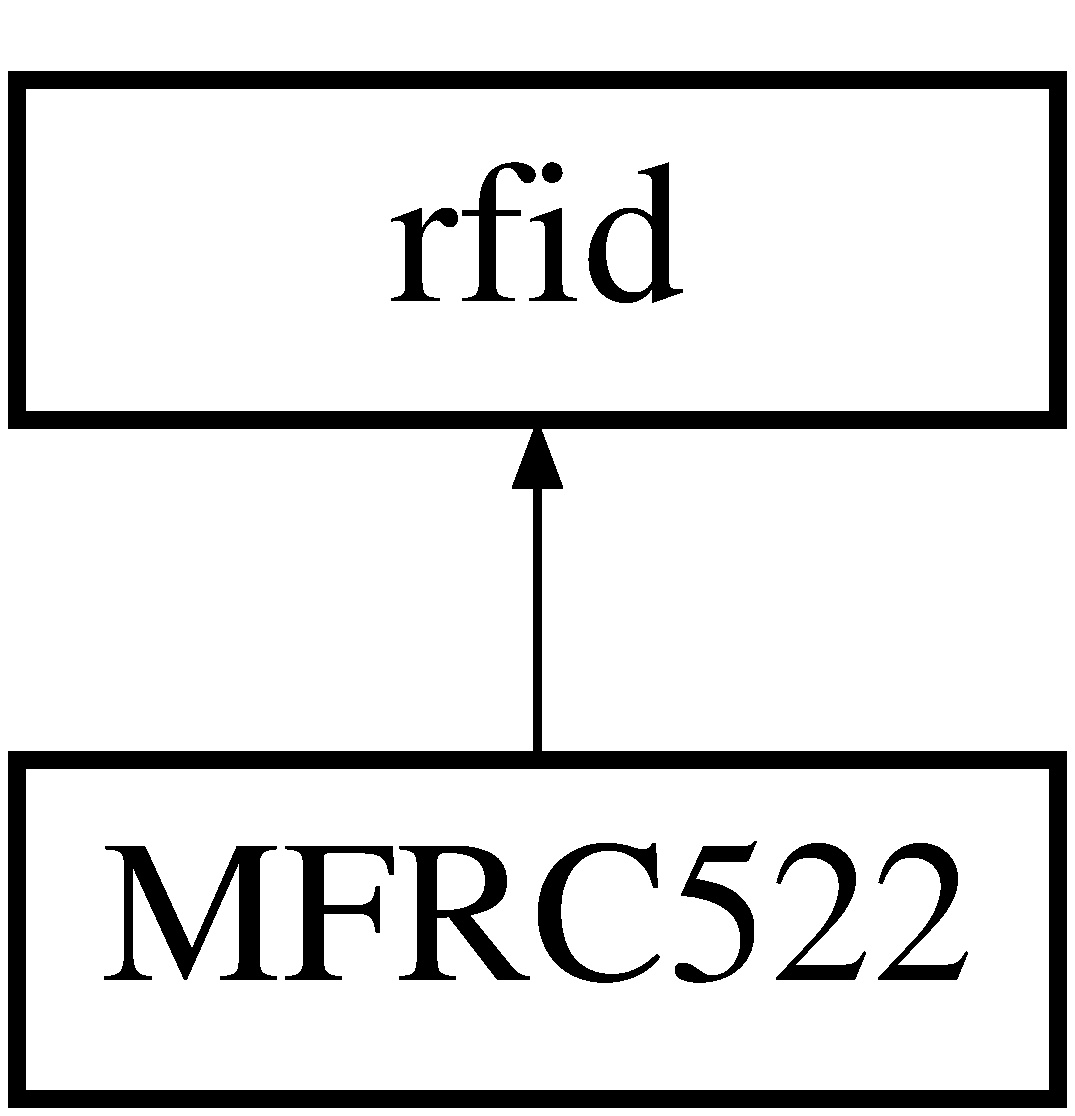
\includegraphics[height=2.000000cm]{class_m_f_r_c522}
\end{center}
\end{figure}
\subsection*{Public Types}
\begin{DoxyCompactItemize}
\item 
enum \mbox{\hyperlink{class_m_f_r_c522_ae7ec09eb8c9c61288a4770175b4b8db7}{R\+EG}} \+: uint8\+\_\+t \{ \newline
{\bfseries R\+E\+S\+E\+R\+V\+E\+D1} = 0x00, 
\mbox{\hyperlink{class_m_f_r_c522_ae7ec09eb8c9c61288a4770175b4b8db7a0ec37643fa721f476b0cd4359e3c7ef1}{Command\+Reg}}, 
\mbox{\hyperlink{class_m_f_r_c522_ae7ec09eb8c9c61288a4770175b4b8db7ad956725472615518dfb99f2d7dccc50e}{Com\+I\+En\+Reg}}, 
\mbox{\hyperlink{class_m_f_r_c522_ae7ec09eb8c9c61288a4770175b4b8db7afb4527cc3e364cce3fe3e62cdcde7da0}{Div\+I\+En\+Reg}}, 
\newline
\mbox{\hyperlink{class_m_f_r_c522_ae7ec09eb8c9c61288a4770175b4b8db7a76b2a615444982e04566784bdb5c9841}{Com\+Irq\+Reg}}, 
\mbox{\hyperlink{class_m_f_r_c522_ae7ec09eb8c9c61288a4770175b4b8db7a95e26d5ece97ae43c34d08797205a356}{Div\+Irq\+Reg}}, 
\mbox{\hyperlink{class_m_f_r_c522_ae7ec09eb8c9c61288a4770175b4b8db7a240aa03a1d9542235b89cdef377a5796}{Error\+Reg}}, 
\mbox{\hyperlink{class_m_f_r_c522_ae7ec09eb8c9c61288a4770175b4b8db7a9f8b10dda6868e74226ab7ccca8d5be0}{Status1\+Reg}}, 
\newline
\mbox{\hyperlink{class_m_f_r_c522_ae7ec09eb8c9c61288a4770175b4b8db7a8fb1a8c28b7a860793831566373f172f}{Status2\+Reg}}, 
\mbox{\hyperlink{class_m_f_r_c522_ae7ec09eb8c9c61288a4770175b4b8db7afdbfd2f397b96d1043c808ec26e80328}{F\+I\+F\+O\+Data\+Reg}}, 
\mbox{\hyperlink{class_m_f_r_c522_ae7ec09eb8c9c61288a4770175b4b8db7a35e5daf30358a0a271dadf50ba6bb4e7}{F\+I\+F\+O\+Level\+Reg}}, 
\mbox{\hyperlink{class_m_f_r_c522_ae7ec09eb8c9c61288a4770175b4b8db7aee5f7c4d0d34d93e5ac67a47e886b224}{Water\+Level\+Reg}}, 
\newline
\mbox{\hyperlink{class_m_f_r_c522_ae7ec09eb8c9c61288a4770175b4b8db7a9d0df9e03ad6706004b003e20127a76a}{Control\+Reg}}, 
\mbox{\hyperlink{class_m_f_r_c522_ae7ec09eb8c9c61288a4770175b4b8db7aaf8beb5a739cd8bf94b8b5c8d2d109ce}{Bit\+Framing\+Reg}}, 
\mbox{\hyperlink{class_m_f_r_c522_ae7ec09eb8c9c61288a4770175b4b8db7afafb7ec88f79c9b1f195195497d0ca07}{Coll\+Reg}}, 
{\bfseries R\+E\+S\+E\+R\+V\+E\+D2}, 
\newline
{\bfseries R\+E\+S\+E\+R\+V\+E\+D3}, 
\mbox{\hyperlink{class_m_f_r_c522_ae7ec09eb8c9c61288a4770175b4b8db7a2cd647ad1ac1327d2a632115cd9c4477}{Mode\+Reg}}, 
\mbox{\hyperlink{class_m_f_r_c522_ae7ec09eb8c9c61288a4770175b4b8db7ad4fe18ad01abc83d4559369226fe7992}{Tx\+Mode\+Reg}}, 
\mbox{\hyperlink{class_m_f_r_c522_ae7ec09eb8c9c61288a4770175b4b8db7a7e0d6ae1fdd25be6d80d1b76b2274764}{Rx\+Mode\+Reg}}, 
\newline
\mbox{\hyperlink{class_m_f_r_c522_ae7ec09eb8c9c61288a4770175b4b8db7a73dc12b03f05177a400263e5e2bcf0cc}{Tx\+Control\+Reg}}, 
\mbox{\hyperlink{class_m_f_r_c522_ae7ec09eb8c9c61288a4770175b4b8db7ac9de33ca066ca9481bd01d5642a0c879}{Tx\+A\+S\+K\+Reg}}, 
\mbox{\hyperlink{class_m_f_r_c522_ae7ec09eb8c9c61288a4770175b4b8db7a6cf11e077148648aaec0492317be5177}{Tx\+Sel\+Reg}}, 
\mbox{\hyperlink{class_m_f_r_c522_ae7ec09eb8c9c61288a4770175b4b8db7a669c0c9418d5437566b4b42da326c05f}{Rx\+Sel\+Reg}}, 
\newline
\mbox{\hyperlink{class_m_f_r_c522_ae7ec09eb8c9c61288a4770175b4b8db7a5dfb7b5c8983d07d7df4fa915902db4c}{rx\+Threshold\+Reg}}, 
\mbox{\hyperlink{class_m_f_r_c522_ae7ec09eb8c9c61288a4770175b4b8db7a37b01e93fff19ca62364e8f4f797a5c4}{Demod\+Reg}}, 
{\bfseries R\+E\+S\+E\+R\+V\+E\+D4}, 
{\bfseries R\+E\+S\+E\+R\+V\+E\+D5}, 
\newline
\mbox{\hyperlink{class_m_f_r_c522_ae7ec09eb8c9c61288a4770175b4b8db7a08eb51f4d08a41ceb4b34189bb712dc7}{Mf\+Tx\+Reg}}, 
\mbox{\hyperlink{class_m_f_r_c522_ae7ec09eb8c9c61288a4770175b4b8db7a92fbf63612de021d242465d4685f1754}{Mf\+Rx\+Reg}}, 
{\bfseries R\+E\+S\+E\+R\+V\+E\+D6}, 
\mbox{\hyperlink{class_m_f_r_c522_ae7ec09eb8c9c61288a4770175b4b8db7a23529258de3c3f5655afa2849f547f68}{Serial\+Speed\+Reg}}, 
\newline
{\bfseries R\+E\+S\+E\+R\+V\+E\+D7}, 
\mbox{\hyperlink{class_m_f_r_c522_ae7ec09eb8c9c61288a4770175b4b8db7a93ba2171ffd0724c539ea656627e3944}{C\+R\+C\+Result1\+Reg}}, 
\mbox{\hyperlink{class_m_f_r_c522_ae7ec09eb8c9c61288a4770175b4b8db7a38946dab95c184fd8ca72747d51dc0c5}{C\+R\+C\+Result2\+Reg}}, 
{\bfseries R\+E\+S\+E\+R\+V\+E\+D8}, 
\newline
\mbox{\hyperlink{class_m_f_r_c522_ae7ec09eb8c9c61288a4770175b4b8db7ad69a6a3d883ebfc993fc6fbdbc035508}{Mod\+Width\+Reg}}, 
{\bfseries R\+E\+S\+E\+R\+V\+E\+D9}, 
\mbox{\hyperlink{class_m_f_r_c522_ae7ec09eb8c9c61288a4770175b4b8db7a0c99eea491c71e9d2a02bf8a86988adf}{R\+F\+Cfg\+Reg}}, 
\mbox{\hyperlink{class_m_f_r_c522_ae7ec09eb8c9c61288a4770175b4b8db7a2f81aa5f433fa51bb4b41cd8955de794}{Gs\+N\+Reg}}, 
\newline
\mbox{\hyperlink{class_m_f_r_c522_ae7ec09eb8c9c61288a4770175b4b8db7a02925dc7a230fcf039c597bf8cfa113f}{C\+W\+Gs\+P\+Reg}}, 
\mbox{\hyperlink{class_m_f_r_c522_ae7ec09eb8c9c61288a4770175b4b8db7acf6ed89766ba2a4e6483b3209b1aa74e}{Mod\+Gs\+P\+Reg}}, 
\mbox{\hyperlink{class_m_f_r_c522_ae7ec09eb8c9c61288a4770175b4b8db7a1ed52e7f88c8bf3fda91bf31bb62afe4}{T\+Mode\+Reg}}, 
\mbox{\hyperlink{class_m_f_r_c522_ae7ec09eb8c9c61288a4770175b4b8db7a88c2ad7cdfb7178ea775c157f4ce5213}{T\+Prescaler\+Reg}}, 
\newline
\mbox{\hyperlink{class_m_f_r_c522_ae7ec09eb8c9c61288a4770175b4b8db7a1b5d7dfad8ec2fbc93d7b7c67cb0d94c}{T\+Reload\+Reg1}}, 
\mbox{\hyperlink{class_m_f_r_c522_ae7ec09eb8c9c61288a4770175b4b8db7a5dbae491d9100c3437ff1ae30873e583}{T\+Reload\+Reg2}}, 
\mbox{\hyperlink{class_m_f_r_c522_ae7ec09eb8c9c61288a4770175b4b8db7af5d128e56733edcb6a36f2e62003b914}{T\+Counter\+Val\+Reg1}}, 
\mbox{\hyperlink{class_m_f_r_c522_ae7ec09eb8c9c61288a4770175b4b8db7a90426989ff0e68a88f71fa5e12da987a}{T\+Counter\+Val\+Reg2}}, 
\newline
{\bfseries R\+E\+S\+E\+R\+V\+E\+D10}, 
\mbox{\hyperlink{class_m_f_r_c522_ae7ec09eb8c9c61288a4770175b4b8db7a3fd81beec1ed6566ff1897aac235890f}{Test\+Sel1\+Reg}}, 
\mbox{\hyperlink{class_m_f_r_c522_ae7ec09eb8c9c61288a4770175b4b8db7ac1053bcb64682eba4a767caaea677807}{Test\+Sel2\+Reg}}, 
\mbox{\hyperlink{class_m_f_r_c522_ae7ec09eb8c9c61288a4770175b4b8db7a62a7871c0d3452a8f642bbea0ca7cb34}{Test\+Pin\+En\+Reg}}, 
\newline
\mbox{\hyperlink{class_m_f_r_c522_ae7ec09eb8c9c61288a4770175b4b8db7aa5bb4445abb525ddf46c6efcb21e8811}{Test\+Pin\+Value\+Reg}}, 
\mbox{\hyperlink{class_m_f_r_c522_ae7ec09eb8c9c61288a4770175b4b8db7a37bc0188996dc1ee5332d40961bffb4b}{Test\+Bus\+Reg}}, 
\mbox{\hyperlink{class_m_f_r_c522_ae7ec09eb8c9c61288a4770175b4b8db7a9583618ad17a8a20b7a735c7677c8e56}{Auto\+Test\+Reg}}, 
\mbox{\hyperlink{class_m_f_r_c522_ae7ec09eb8c9c61288a4770175b4b8db7a4281c25cf6743163ed2e2f903cf17ba9}{Version\+Reg}}, 
\newline
\mbox{\hyperlink{class_m_f_r_c522_ae7ec09eb8c9c61288a4770175b4b8db7af1d5966b064c10a672e0064d3ccc55c3}{Analog\+Test\+Reg}}, 
\mbox{\hyperlink{class_m_f_r_c522_ae7ec09eb8c9c61288a4770175b4b8db7a25334abb5ff680a530e95e6fb0e48a5b}{Test\+D\+A\+C1\+Reg}}, 
\mbox{\hyperlink{class_m_f_r_c522_ae7ec09eb8c9c61288a4770175b4b8db7a505b75aac860302b2959da7fe607e5eb}{Test\+D\+A\+C2\+Reg}}, 
\mbox{\hyperlink{class_m_f_r_c522_ae7ec09eb8c9c61288a4770175b4b8db7a1042587aeb71f82f884975ca54c8854a}{Test\+A\+D\+C\+Reg}}
 \}
\begin{DoxyCompactList}\small\item\em All the internal register used in the \mbox{\hyperlink{class_m_f_r_c522}{M\+F\+R\+C522}} chip. \end{DoxyCompactList}\item 
enum \mbox{\hyperlink{class_m_f_r_c522_abf038692c9cf33ed59b44a612e6ed1c7}{C\+O\+M\+M\+A\+ND}} \+: uint8\+\_\+t \{ \newline
{\bfseries Idle} = 0x00, 
{\bfseries Mem}, 
{\bfseries Generate\+\_\+\+Random\+ID}, 
{\bfseries Calc\+C\+RC}, 
\newline
{\bfseries No\+Cmd\+Change} = 0x07, 
{\bfseries Receive}, 
{\bfseries Transceive} = 0x0C, 
{\bfseries M\+F\+Authent} = 0x0E, 
\newline
{\bfseries Soft\+Reset}
 \}
\begin{DoxyCompactList}\small\item\em The possible commands the \mbox{\hyperlink{class_m_f_r_c522}{M\+F\+R\+C522}} has. \end{DoxyCompactList}\item 
enum \mbox{\hyperlink{class_m_f_r_c522_a79bd44224bb1ad85e28a0937a6715818}{M\+I\+F\+A\+R\+E\+\_\+\+C\+O\+M\+M\+A\+ND}} \+: uint8\+\_\+t \{ \newline
{\bfseries Request\+Command} = 0x26, 
{\bfseries Wake\+Up\+Command} = 0x52, 
{\bfseries C\+L1\+Command} = 0x93, 
{\bfseries C\+L2\+Command} = 0x95, 
\newline
{\bfseries Anticollision\+Command} = 0x20, 
{\bfseries Select\+Command} = 0x70, 
{\bfseries Halt\+Part1\+Command} = 0x50, 
{\bfseries Halt\+Part2\+Command} = 0x00, 
\newline
{\bfseries Auth\+Key\+A\+Command} = 0x60, 
{\bfseries Auth\+Key\+B\+Command} = 0x61, 
{\bfseries Personalize\+U\+I\+D\+Usage\+Command} = 0x40, 
{\bfseries Set\+Mod\+Type\+Command} = 0x43, 
\newline
{\bfseries Read\+Command} = 0x30, 
{\bfseries Write\+Command} = 0x\+A0, 
{\bfseries Decrement\+Command} = 0x\+C0, 
{\bfseries Increment\+Command} = 0x\+C1, 
\newline
{\bfseries Restore\+Command} = 0x\+C2, 
{\bfseries Transfer\+Command} = 0x\+B0
 \}
\begin{DoxyCompactList}\small\item\em All the M\+I\+F\+A\+RE Classic E\+V1 with 1K commands. \end{DoxyCompactList}\item 
enum \mbox{\hyperlink{class_m_f_r_c522_a1160642f3b2b60b5ea7309374a8d760a}{C\+O\+M\+M\+U\+N\+I\+C\+A\+T\+I\+O\+N\+\_\+\+S\+T\+A\+T\+US}} \+: uint8\+\_\+t \{ \newline
{\bfseries Ok\+Status}, 
{\bfseries Time\+Out\+Status}, 
{\bfseries No\+Room}, 
{\bfseries Protocol\+Err}, 
\newline
{\bfseries Parity\+Err}, 
{\bfseries C\+R\+C\+Err}, 
{\bfseries Coll\+Err}, 
{\bfseries Buffer\+Ovfl}, 
\newline
{\bfseries Temp\+Err}, 
{\bfseries Wr\+Err}, 
{\bfseries B\+C\+C\+Err}
 \}
\begin{DoxyCompactList}\small\item\em All the communication status values. \end{DoxyCompactList}\end{DoxyCompactItemize}
\subsection*{Public Member Functions}
\begin{DoxyCompactItemize}
\item 
\mbox{\hyperlink{class_m_f_r_c522_a70e6c463aec08918c71c2e0c77742b4b}{M\+F\+R\+C522}} (\mbox{\hyperlink{classspi_bus}{spi\+Bus}} \&S\+P\+I\+Bus, hwlib\+::pin\+\_\+out \&slave\+Select, hwlib\+::pin\+\_\+out \&reset, bool init=true)
\begin{DoxyCompactList}\small\item\em \mbox{\hyperlink{class_m_f_r_c522}{M\+F\+R\+C522}} class constructor. \end{DoxyCompactList}\item 
void \mbox{\hyperlink{class_m_f_r_c522_a5f589b09eaf150551b369052ce125fa1}{initialize}} () override
\begin{DoxyCompactList}\small\item\em Initialize the rfid chip for. \end{DoxyCompactList}\item 
void \mbox{\hyperlink{class_m_f_r_c522_a016df9ed0421397c634cc79c475dbe3b}{hard\+Reset}} () override
\begin{DoxyCompactList}\small\item\em Hard reset the rfid chip probably with a hwlib\+::pin\+\_\+out (\href{mailto:wouter@voti.nl}{\tt wouter@voti.\+nl}) 2017. \end{DoxyCompactList}\item 
\mbox{\Hypertarget{class_m_f_r_c522_ae51e1e0bee2b7a65d6314bfb48121f1d}\label{class_m_f_r_c522_ae51e1e0bee2b7a65d6314bfb48121f1d}} 
void \mbox{\hyperlink{class_m_f_r_c522_ae51e1e0bee2b7a65d6314bfb48121f1d}{soft\+Reset}} () override
\begin{DoxyCompactList}\small\item\em Soft reset the rfid chip. \end{DoxyCompactList}\item 
void \mbox{\hyperlink{class_m_f_r_c522_ac981022cc3ae79f727b2365e309cf691}{reset\+Antennas}} () override
\begin{DoxyCompactList}\small\item\em Reset the Tx and Rx antennas. \end{DoxyCompactList}\item 
bool \mbox{\hyperlink{class_m_f_r_c522_a019f76569bddf9c2f9f94eca13a618d7}{is\+Card\+In\+Range}} () override
\begin{DoxyCompactList}\small\item\em Check if there is a card within the radio frequency field. \end{DoxyCompactList}\item 
bool \mbox{\hyperlink{class_m_f_r_c522_a29ce0dd04495f9352e32ada5ecc5fd03}{is\+Card\+In\+Range\+Check}} () override
\begin{DoxyCompactList}\small\item\em Check if there is a card within the radio frequency field. \end{DoxyCompactList}\item 
uint8\+\_\+t \mbox{\hyperlink{class_m_f_r_c522_ad3c7ab4c70988e80c400f36f724a12b7}{get\+Card\+U\+ID}} (uint8\+\_\+t U\+ID\mbox{[}5\mbox{]}) override
\begin{DoxyCompactList}\small\item\em Get the U\+I\+D/\+N\+U\+ID of 4 bytes U\+ID card with the B\+CC byte. \end{DoxyCompactList}\item 
bool \mbox{\hyperlink{class_m_f_r_c522_a33c20be6030f635d986984db4999a1eb}{get\+Card\+U\+I\+D\+Simple}} (uint8\+\_\+t U\+ID\mbox{[}5\mbox{]}) override
\begin{DoxyCompactList}\small\item\em A wrapper around \mbox{\hyperlink{class_m_f_r_c522_ad3c7ab4c70988e80c400f36f724a12b7}{get\+Card\+U\+ID}} to make it simpler. \end{DoxyCompactList}\item 
void \mbox{\hyperlink{class_m_f_r_c522_aeb05c83c2d139eb2c57f400399982691}{wait\+For\+Card\+U\+ID}} (uint8\+\_\+t U\+ID\mbox{[}5\mbox{]}) override
\begin{DoxyCompactList}\small\item\em This function waits till there is a card in range and gives the U\+ID back. \end{DoxyCompactList}\item 
uint8\+\_\+t \mbox{\hyperlink{class_m_f_r_c522_a25fb0a50bf7db51ab9c5bc2ff4fa84e3}{get\+Version}} () override
\begin{DoxyCompactList}\small\item\em Get the version of the rfid chip to perform for instance a \mbox{\hyperlink{class_m_f_r_c522_adcc4f5eb212c1a94e462eab459bd685e}{self\+Test}}. \end{DoxyCompactList}\item 
bool \mbox{\hyperlink{class_m_f_r_c522_adcc4f5eb212c1a94e462eab459bd685e}{self\+Test}} () override
\begin{DoxyCompactList}\small\item\em Let the rfid chip perform a self test. \end{DoxyCompactList}\end{DoxyCompactItemize}
\subsection*{Public Attributes}
\begin{DoxyCompactItemize}
\item 
\mbox{\Hypertarget{class_m_f_r_c522_a56c8309a003cf1a5d8479c7783826f8e}\label{class_m_f_r_c522_a56c8309a003cf1a5d8479c7783826f8e}} 
const uint8\+\_\+t \mbox{\hyperlink{class_m_f_r_c522_a56c8309a003cf1a5d8479c7783826f8e}{F\+I\+F\+O\+Amount\+Of\+Bytes}} = 64
\begin{DoxyCompactList}\small\item\em The maximum amount of bytes the F\+I\+FO can store. \end{DoxyCompactList}\item 
const uint8\+\_\+t \mbox{\hyperlink{class_m_f_r_c522_a7d19c9869a7fbbe0d9825d5653d6af7b}{self\+Test\+F\+I\+F\+O\+Buffer\+V1}} \mbox{[}64\mbox{]}
\begin{DoxyCompactList}\small\item\em The data that will be in the F\+I\+FO after executing the self\+Test on a \mbox{\hyperlink{class_m_f_r_c522}{M\+F\+R\+C522}} version 1. \end{DoxyCompactList}\item 
const uint8\+\_\+t \mbox{\hyperlink{class_m_f_r_c522_a6973b73a8a922ac09b9d89489bdbc333}{self\+Test\+F\+I\+F\+O\+Buffer\+V2}} \mbox{[}64\mbox{]}
\begin{DoxyCompactList}\small\item\em The data that will be in the F\+I\+FO after executing the self\+Test on a \mbox{\hyperlink{class_m_f_r_c522}{M\+F\+R\+C522}} version 2. \end{DoxyCompactList}\end{DoxyCompactItemize}
\subsection*{Protected Member Functions}
\begin{DoxyCompactItemize}
\item 
\mbox{\Hypertarget{class_m_f_r_c522_a6bfefd877c6060dde4eff2c25b7f96f2}\label{class_m_f_r_c522_a6bfefd877c6060dde4eff2c25b7f96f2}} 
void \mbox{\hyperlink{class_m_f_r_c522_a6bfefd877c6060dde4eff2c25b7f96f2}{wait\+Till\+Started}} () override
\begin{DoxyCompactList}\small\item\em Wait till the is started correctly after for example a soft reset. \end{DoxyCompactList}\item 
\mbox{\Hypertarget{class_m_f_r_c522_afe0e86db047ef36af49349e7fdc7fa65}\label{class_m_f_r_c522_afe0e86db047ef36af49349e7fdc7fa65}} 
uint8\+\_\+t {\bfseries read\+Register} (\mbox{\hyperlink{class_m_f_r_c522_ae7ec09eb8c9c61288a4770175b4b8db7}{R\+EG}} register\+Address)
\item 
\mbox{\Hypertarget{class_m_f_r_c522_a559408e38c2c8fea3316f6e2b4477b81}\label{class_m_f_r_c522_a559408e38c2c8fea3316f6e2b4477b81}} 
void {\bfseries read\+Register} (\mbox{\hyperlink{class_m_f_r_c522_ae7ec09eb8c9c61288a4770175b4b8db7}{R\+EG}} register\+Address, uint8\+\_\+t read\mbox{[}$\,$\mbox{]}, uint8\+\_\+t amount\+Of\+Bytes)
\item 
\mbox{\Hypertarget{class_m_f_r_c522_aa976c78dde5b2dfbbd5bcbedaad14a7a}\label{class_m_f_r_c522_aa976c78dde5b2dfbbd5bcbedaad14a7a}} 
void {\bfseries write\+Register} (\mbox{\hyperlink{class_m_f_r_c522_ae7ec09eb8c9c61288a4770175b4b8db7}{R\+EG}} register\+Address, uint8\+\_\+t new\+Byte)
\item 
\mbox{\Hypertarget{class_m_f_r_c522_a3558d379575863072c711721b061bb75}\label{class_m_f_r_c522_a3558d379575863072c711721b061bb75}} 
void {\bfseries write\+Register} (\mbox{\hyperlink{class_m_f_r_c522_ae7ec09eb8c9c61288a4770175b4b8db7}{R\+EG}} register\+Address, uint8\+\_\+t new\+Bytes\mbox{[}$\,$\mbox{]}, int amount\+Of\+Bytes)
\item 
\mbox{\Hypertarget{class_m_f_r_c522_ae30686cdd50f6fdb821908a2547e5153}\label{class_m_f_r_c522_ae30686cdd50f6fdb821908a2547e5153}} 
void {\bfseries set\+Mask\+In\+Register} (\mbox{\hyperlink{class_m_f_r_c522_ae7ec09eb8c9c61288a4770175b4b8db7}{R\+EG}} register\+Address, uint8\+\_\+t mask)
\item 
\mbox{\Hypertarget{class_m_f_r_c522_a9935264b559702a3a4ad2b87735b4f8f}\label{class_m_f_r_c522_a9935264b559702a3a4ad2b87735b4f8f}} 
void {\bfseries clear\+Mask\+In\+Register} (\mbox{\hyperlink{class_m_f_r_c522_ae7ec09eb8c9c61288a4770175b4b8db7}{R\+EG}} register\+Address, uint8\+\_\+t mask)
\item 
\mbox{\Hypertarget{class_m_f_r_c522_ad33cc8218440b30747fba97aa59c0583}\label{class_m_f_r_c522_ad33cc8218440b30747fba97aa59c0583}} 
void {\bfseries set\+Antennas} (bool state)
\item 
\mbox{\Hypertarget{class_m_f_r_c522_a4df3a992241adac22f7e0464471c3b94}\label{class_m_f_r_c522_a4df3a992241adac22f7e0464471c3b94}} 
void {\bfseries calculate\+C\+RC} (uint8\+\_\+t $\ast$data, int len, uint8\+\_\+t $\ast$result)
\item 
\mbox{\Hypertarget{class_m_f_r_c522_a6d831a60a08c5f37a264c61f7c79c372}\label{class_m_f_r_c522_a6d831a60a08c5f37a264c61f7c79c372}} 
uint8\+\_\+t {\bfseries check\+For\+Errors} ()
\item 
\mbox{\Hypertarget{class_m_f_r_c522_ab605cd58a59f1d6cbc48ef0be252e593}\label{class_m_f_r_c522_ab605cd58a59f1d6cbc48ef0be252e593}} 
uint8\+\_\+t {\bfseries communicate} (\mbox{\hyperlink{class_m_f_r_c522_abf038692c9cf33ed59b44a612e6ed1c7}{C\+O\+M\+M\+A\+ND}} command, uint8\+\_\+t transmit\+Data\mbox{[}$\,$\mbox{]}, int transmit\+Length, uint8\+\_\+t received\+Data\mbox{[}$\,$\mbox{]}, int \&received\+Length)
\end{DoxyCompactItemize}
\subsection*{Private Member Functions}
\begin{DoxyCompactItemize}
\item 
\mbox{\Hypertarget{class_m_f_r_c522_a0fa1703360d0c741cf915b22e26c2631}\label{class_m_f_r_c522_a0fa1703360d0c741cf915b22e26c2631}} 
void {\bfseries clear\+F\+I\+F\+O\+Buffer} (const uint8\+\_\+t amount\+Of\+Bytes=64)
\item 
\mbox{\Hypertarget{class_m_f_r_c522_a9d2c5ad7b977944e8bcbbcc9c1bb9b75}\label{class_m_f_r_c522_a9d2c5ad7b977944e8bcbbcc9c1bb9b75}} 
void {\bfseries clear\+Internal\+Buffer} ()
\end{DoxyCompactItemize}
\subsection*{Private Attributes}
\begin{DoxyCompactItemize}
\item 
\mbox{\Hypertarget{class_m_f_r_c522_a76b0186fcad01aafd3d7d7ae4da6a68c}\label{class_m_f_r_c522_a76b0186fcad01aafd3d7d7ae4da6a68c}} 
\mbox{\hyperlink{classspi_bus}{spi\+Bus}} \& {\bfseries S\+P\+I\+Bus}
\item 
\mbox{\Hypertarget{class_m_f_r_c522_ab945c275a8644e226def9f3eee6698a2}\label{class_m_f_r_c522_ab945c275a8644e226def9f3eee6698a2}} 
hwlib\+::pin\+\_\+out \& {\bfseries slave\+Select}
\item 
\mbox{\Hypertarget{class_m_f_r_c522_a924c7dced5cb615461a0c9f353076407}\label{class_m_f_r_c522_a924c7dced5cb615461a0c9f353076407}} 
hwlib\+::pin\+\_\+out \& {\bfseries reset}
\end{DoxyCompactItemize}


\subsection{Detailed Description}
This class is used to communicate with the \mbox{\hyperlink{class_m_f_r_c522}{M\+F\+R\+C522}} chip. 

This is a basic library for the M\+F522 chip. Using the pure virtual class \mbox{\hyperlink{classrfid}{rfid}}. Execute the tests when you\textquotesingle{}re not sure the chip is connected correctly. \begin{DoxyWarning}{Warning}
T\+HE S\+O\+F\+T\+W\+A\+RE IS P\+R\+O\+V\+I\+D\+ED \char`\"{}\+A\+S I\+S\char`\"{}, W\+I\+T\+H\+O\+UT W\+A\+R\+R\+A\+N\+TY OF A\+NY K\+I\+ND. 
\end{DoxyWarning}


\subsection{Member Enumeration Documentation}
\mbox{\Hypertarget{class_m_f_r_c522_abf038692c9cf33ed59b44a612e6ed1c7}\label{class_m_f_r_c522_abf038692c9cf33ed59b44a612e6ed1c7}} 
\index{M\+F\+R\+C522@{M\+F\+R\+C522}!C\+O\+M\+M\+A\+ND@{C\+O\+M\+M\+A\+ND}}
\index{C\+O\+M\+M\+A\+ND@{C\+O\+M\+M\+A\+ND}!M\+F\+R\+C522@{M\+F\+R\+C522}}
\subsubsection{\texorpdfstring{C\+O\+M\+M\+A\+ND}{COMMAND}}
{\footnotesize\ttfamily enum \mbox{\hyperlink{class_m_f_r_c522_abf038692c9cf33ed59b44a612e6ed1c7}{M\+F\+R\+C522\+::\+C\+O\+M\+M\+A\+ND}} \+: uint8\+\_\+t}



The possible commands the \mbox{\hyperlink{class_m_f_r_c522}{M\+F\+R\+C522}} has. 

Before using these commands you should have some basic knowledge of what they do. Check the datasheet before using! \begin{DoxySeeAlso}{See also}
\href{https://www.nxp.com/docs/en/data-sheet/MFRC522.pdf}{\tt M\+F\+R\+C522 datasheet page 70} 
\end{DoxySeeAlso}
\begin{DoxyWarning}{Warning}
Check the datasheet before using! 
\end{DoxyWarning}
\mbox{\Hypertarget{class_m_f_r_c522_a1160642f3b2b60b5ea7309374a8d760a}\label{class_m_f_r_c522_a1160642f3b2b60b5ea7309374a8d760a}} 
\index{M\+F\+R\+C522@{M\+F\+R\+C522}!C\+O\+M\+M\+U\+N\+I\+C\+A\+T\+I\+O\+N\+\_\+\+S\+T\+A\+T\+US@{C\+O\+M\+M\+U\+N\+I\+C\+A\+T\+I\+O\+N\+\_\+\+S\+T\+A\+T\+US}}
\index{C\+O\+M\+M\+U\+N\+I\+C\+A\+T\+I\+O\+N\+\_\+\+S\+T\+A\+T\+US@{C\+O\+M\+M\+U\+N\+I\+C\+A\+T\+I\+O\+N\+\_\+\+S\+T\+A\+T\+US}!M\+F\+R\+C522@{M\+F\+R\+C522}}
\subsubsection{\texorpdfstring{C\+O\+M\+M\+U\+N\+I\+C\+A\+T\+I\+O\+N\+\_\+\+S\+T\+A\+T\+US}{COMMUNICATION\_STATUS}}
{\footnotesize\ttfamily enum \mbox{\hyperlink{class_m_f_r_c522_a1160642f3b2b60b5ea7309374a8d760a}{M\+F\+R\+C522\+::\+C\+O\+M\+M\+U\+N\+I\+C\+A\+T\+I\+O\+N\+\_\+\+S\+T\+A\+T\+US}} \+: uint8\+\_\+t}



All the communication status values. 

Ok\+Status is the best status you can have! Everything went fine! Time\+Out\+Status happens when the timer is down to 0 after for example transmitting the bytes to the card. ~\newline
~\newline
 No\+Room occurs when the passed array is smaller than the amount of bytes received in the \mbox{\hyperlink{class_m_f_r_c522_ae7ec09eb8c9c61288a4770175b4b8db7afdbfd2f397b96d1043c808ec26e80328}{F\+I\+F\+O\+Data\+Reg}}. (check using \mbox{\hyperlink{class_m_f_r_c522_ae7ec09eb8c9c61288a4770175b4b8db7a35e5daf30358a0a271dadf50ba6bb4e7}{F\+I\+F\+O\+Level\+Reg}}) ~\newline
~\newline
 After for example transceiving the M\+F\+R\+C52 does serveral checks. The results are stored in the \#error\+Reg. Any status ending with Err is an Error! \mbox{\Hypertarget{class_m_f_r_c522_a79bd44224bb1ad85e28a0937a6715818}\label{class_m_f_r_c522_a79bd44224bb1ad85e28a0937a6715818}} 
\index{M\+F\+R\+C522@{M\+F\+R\+C522}!M\+I\+F\+A\+R\+E\+\_\+\+C\+O\+M\+M\+A\+ND@{M\+I\+F\+A\+R\+E\+\_\+\+C\+O\+M\+M\+A\+ND}}
\index{M\+I\+F\+A\+R\+E\+\_\+\+C\+O\+M\+M\+A\+ND@{M\+I\+F\+A\+R\+E\+\_\+\+C\+O\+M\+M\+A\+ND}!M\+F\+R\+C522@{M\+F\+R\+C522}}
\subsubsection{\texorpdfstring{M\+I\+F\+A\+R\+E\+\_\+\+C\+O\+M\+M\+A\+ND}{MIFARE\_COMMAND}}
{\footnotesize\ttfamily enum \mbox{\hyperlink{class_m_f_r_c522_a79bd44224bb1ad85e28a0937a6715818}{M\+F\+R\+C522\+::\+M\+I\+F\+A\+R\+E\+\_\+\+C\+O\+M\+M\+A\+ND}} \+: uint8\+\_\+t}



All the M\+I\+F\+A\+RE Classic E\+V1 with 1K commands. 

Most of the commands are M\+I\+F\+A\+RE Classic only. But some are defined in the I\+S\+O/\+I\+EC 14443 Type A. So some command might be used for more card like the request and wake-\/up command. For more information about the M\+I\+F\+A\+RE command take a look at the datasheet. Most M\+I\+F\+A\+RE commands require authentication! \href{http://www.orangetags.com/wp-content/downloads/datasheet/NXP/Mifare%20EV1%201K.pdf}{\tt M\+I\+F\+A\+RE datsheet page 13} \begin{DoxyWarning}{Warning}
some commands override the data on the cards! W\+A\+T\+CH O\+U\+T! 
\end{DoxyWarning}
\mbox{\Hypertarget{class_m_f_r_c522_ae7ec09eb8c9c61288a4770175b4b8db7}\label{class_m_f_r_c522_ae7ec09eb8c9c61288a4770175b4b8db7}} 
\index{M\+F\+R\+C522@{M\+F\+R\+C522}!R\+EG@{R\+EG}}
\index{R\+EG@{R\+EG}!M\+F\+R\+C522@{M\+F\+R\+C522}}
\subsubsection{\texorpdfstring{R\+EG}{REG}}
{\footnotesize\ttfamily enum \mbox{\hyperlink{class_m_f_r_c522_ae7ec09eb8c9c61288a4770175b4b8db7}{M\+F\+R\+C522\+::\+R\+EG}} \+: uint8\+\_\+t}



All the internal register used in the \mbox{\hyperlink{class_m_f_r_c522}{M\+F\+R\+C522}} chip. 

The enums contains all the reigsters in the \mbox{\hyperlink{class_m_f_r_c522}{M\+F\+R\+C522}} chip. For more information about all the registers you should check the datasheet. \begin{DoxySeeAlso}{See also}
\href{https://www.nxp.com/docs/en/data-sheet/MFRC522.pdf}{\tt M\+F\+R\+C522 datasheet page 36} 
\end{DoxySeeAlso}
\begin{DoxyEnumFields}{Enumerator}
\raisebox{\heightof{T}}[0pt][0pt]{\index{Command\+Reg@{Command\+Reg}!M\+F\+R\+C522@{M\+F\+R\+C522}}\index{M\+F\+R\+C522@{M\+F\+R\+C522}!Command\+Reg@{Command\+Reg}}}\mbox{\Hypertarget{class_m_f_r_c522_ae7ec09eb8c9c61288a4770175b4b8db7a0ec37643fa721f476b0cd4359e3c7ef1}\label{class_m_f_r_c522_ae7ec09eb8c9c61288a4770175b4b8db7a0ec37643fa721f476b0cd4359e3c7ef1}} 
Command\+Reg&Starts/stops command execution ~\newline
 \\
\hline

\raisebox{\heightof{T}}[0pt][0pt]{\index{Com\+I\+En\+Reg@{Com\+I\+En\+Reg}!M\+F\+R\+C522@{M\+F\+R\+C522}}\index{M\+F\+R\+C522@{M\+F\+R\+C522}!Com\+I\+En\+Reg@{Com\+I\+En\+Reg}}}\mbox{\Hypertarget{class_m_f_r_c522_ae7ec09eb8c9c61288a4770175b4b8db7ad956725472615518dfb99f2d7dccc50e}\label{class_m_f_r_c522_ae7ec09eb8c9c61288a4770175b4b8db7ad956725472615518dfb99f2d7dccc50e}} 
Com\+I\+En\+Reg&Enable/disable interrupt request control bits. \\
\hline

\raisebox{\heightof{T}}[0pt][0pt]{\index{Div\+I\+En\+Reg@{Div\+I\+En\+Reg}!M\+F\+R\+C522@{M\+F\+R\+C522}}\index{M\+F\+R\+C522@{M\+F\+R\+C522}!Div\+I\+En\+Reg@{Div\+I\+En\+Reg}}}\mbox{\Hypertarget{class_m_f_r_c522_ae7ec09eb8c9c61288a4770175b4b8db7afb4527cc3e364cce3fe3e62cdcde7da0}\label{class_m_f_r_c522_ae7ec09eb8c9c61288a4770175b4b8db7afb4527cc3e364cce3fe3e62cdcde7da0}} 
Div\+I\+En\+Reg&Enable/disable interrupt request control bits. \\
\hline

\raisebox{\heightof{T}}[0pt][0pt]{\index{Com\+Irq\+Reg@{Com\+Irq\+Reg}!M\+F\+R\+C522@{M\+F\+R\+C522}}\index{M\+F\+R\+C522@{M\+F\+R\+C522}!Com\+Irq\+Reg@{Com\+Irq\+Reg}}}\mbox{\Hypertarget{class_m_f_r_c522_ae7ec09eb8c9c61288a4770175b4b8db7a76b2a615444982e04566784bdb5c9841}\label{class_m_f_r_c522_ae7ec09eb8c9c61288a4770175b4b8db7a76b2a615444982e04566784bdb5c9841}} 
Com\+Irq\+Reg&interrupt request bits \\
\hline

\raisebox{\heightof{T}}[0pt][0pt]{\index{Div\+Irq\+Reg@{Div\+Irq\+Reg}!M\+F\+R\+C522@{M\+F\+R\+C522}}\index{M\+F\+R\+C522@{M\+F\+R\+C522}!Div\+Irq\+Reg@{Div\+Irq\+Reg}}}\mbox{\Hypertarget{class_m_f_r_c522_ae7ec09eb8c9c61288a4770175b4b8db7a95e26d5ece97ae43c34d08797205a356}\label{class_m_f_r_c522_ae7ec09eb8c9c61288a4770175b4b8db7a95e26d5ece97ae43c34d08797205a356}} 
Div\+Irq\+Reg&interrupt request bits \\
\hline

\raisebox{\heightof{T}}[0pt][0pt]{\index{Error\+Reg@{Error\+Reg}!M\+F\+R\+C522@{M\+F\+R\+C522}}\index{M\+F\+R\+C522@{M\+F\+R\+C522}!Error\+Reg@{Error\+Reg}}}\mbox{\Hypertarget{class_m_f_r_c522_ae7ec09eb8c9c61288a4770175b4b8db7a240aa03a1d9542235b89cdef377a5796}\label{class_m_f_r_c522_ae7ec09eb8c9c61288a4770175b4b8db7a240aa03a1d9542235b89cdef377a5796}} 
Error\+Reg&Error bits, error status of last command. \\
\hline

\raisebox{\heightof{T}}[0pt][0pt]{\index{Status1\+Reg@{Status1\+Reg}!M\+F\+R\+C522@{M\+F\+R\+C522}}\index{M\+F\+R\+C522@{M\+F\+R\+C522}!Status1\+Reg@{Status1\+Reg}}}\mbox{\Hypertarget{class_m_f_r_c522_ae7ec09eb8c9c61288a4770175b4b8db7a9f8b10dda6868e74226ab7ccca8d5be0}\label{class_m_f_r_c522_ae7ec09eb8c9c61288a4770175b4b8db7a9f8b10dda6868e74226ab7ccca8d5be0}} 
Status1\+Reg&Communication status bits. \\
\hline

\raisebox{\heightof{T}}[0pt][0pt]{\index{Status2\+Reg@{Status2\+Reg}!M\+F\+R\+C522@{M\+F\+R\+C522}}\index{M\+F\+R\+C522@{M\+F\+R\+C522}!Status2\+Reg@{Status2\+Reg}}}\mbox{\Hypertarget{class_m_f_r_c522_ae7ec09eb8c9c61288a4770175b4b8db7a8fb1a8c28b7a860793831566373f172f}\label{class_m_f_r_c522_ae7ec09eb8c9c61288a4770175b4b8db7a8fb1a8c28b7a860793831566373f172f}} 
Status2\+Reg&Receiver and transmitter status bits. \\
\hline

\raisebox{\heightof{T}}[0pt][0pt]{\index{F\+I\+F\+O\+Data\+Reg@{F\+I\+F\+O\+Data\+Reg}!M\+F\+R\+C522@{M\+F\+R\+C522}}\index{M\+F\+R\+C522@{M\+F\+R\+C522}!F\+I\+F\+O\+Data\+Reg@{F\+I\+F\+O\+Data\+Reg}}}\mbox{\Hypertarget{class_m_f_r_c522_ae7ec09eb8c9c61288a4770175b4b8db7afdbfd2f397b96d1043c808ec26e80328}\label{class_m_f_r_c522_ae7ec09eb8c9c61288a4770175b4b8db7afdbfd2f397b96d1043c808ec26e80328}} 
F\+I\+F\+O\+Data\+Reg&Input/output of 64 uint8\+\_\+t F\+I\+FO buffer. \\
\hline

\raisebox{\heightof{T}}[0pt][0pt]{\index{F\+I\+F\+O\+Level\+Reg@{F\+I\+F\+O\+Level\+Reg}!M\+F\+R\+C522@{M\+F\+R\+C522}}\index{M\+F\+R\+C522@{M\+F\+R\+C522}!F\+I\+F\+O\+Level\+Reg@{F\+I\+F\+O\+Level\+Reg}}}\mbox{\Hypertarget{class_m_f_r_c522_ae7ec09eb8c9c61288a4770175b4b8db7a35e5daf30358a0a271dadf50ba6bb4e7}\label{class_m_f_r_c522_ae7ec09eb8c9c61288a4770175b4b8db7a35e5daf30358a0a271dadf50ba6bb4e7}} 
F\+I\+F\+O\+Level\+Reg&Number of uint8\+\_\+t stored in the F\+I\+FO buffer. \\
\hline

\raisebox{\heightof{T}}[0pt][0pt]{\index{Water\+Level\+Reg@{Water\+Level\+Reg}!M\+F\+R\+C522@{M\+F\+R\+C522}}\index{M\+F\+R\+C522@{M\+F\+R\+C522}!Water\+Level\+Reg@{Water\+Level\+Reg}}}\mbox{\Hypertarget{class_m_f_r_c522_ae7ec09eb8c9c61288a4770175b4b8db7aee5f7c4d0d34d93e5ac67a47e886b224}\label{class_m_f_r_c522_ae7ec09eb8c9c61288a4770175b4b8db7aee5f7c4d0d34d93e5ac67a47e886b224}} 
Water\+Level\+Reg&Level for F\+I\+FO underflow and overflow warning. \\
\hline

\raisebox{\heightof{T}}[0pt][0pt]{\index{Control\+Reg@{Control\+Reg}!M\+F\+R\+C522@{M\+F\+R\+C522}}\index{M\+F\+R\+C522@{M\+F\+R\+C522}!Control\+Reg@{Control\+Reg}}}\mbox{\Hypertarget{class_m_f_r_c522_ae7ec09eb8c9c61288a4770175b4b8db7a9d0df9e03ad6706004b003e20127a76a}\label{class_m_f_r_c522_ae7ec09eb8c9c61288a4770175b4b8db7a9d0df9e03ad6706004b003e20127a76a}} 
Control\+Reg&Miscellaneous control register. \\
\hline

\raisebox{\heightof{T}}[0pt][0pt]{\index{Bit\+Framing\+Reg@{Bit\+Framing\+Reg}!M\+F\+R\+C522@{M\+F\+R\+C522}}\index{M\+F\+R\+C522@{M\+F\+R\+C522}!Bit\+Framing\+Reg@{Bit\+Framing\+Reg}}}\mbox{\Hypertarget{class_m_f_r_c522_ae7ec09eb8c9c61288a4770175b4b8db7aaf8beb5a739cd8bf94b8b5c8d2d109ce}\label{class_m_f_r_c522_ae7ec09eb8c9c61288a4770175b4b8db7aaf8beb5a739cd8bf94b8b5c8d2d109ce}} 
Bit\+Framing\+Reg&Adjustments for bit-\/oriented frames. \\
\hline

\raisebox{\heightof{T}}[0pt][0pt]{\index{Coll\+Reg@{Coll\+Reg}!M\+F\+R\+C522@{M\+F\+R\+C522}}\index{M\+F\+R\+C522@{M\+F\+R\+C522}!Coll\+Reg@{Coll\+Reg}}}\mbox{\Hypertarget{class_m_f_r_c522_ae7ec09eb8c9c61288a4770175b4b8db7afafb7ec88f79c9b1f195195497d0ca07}\label{class_m_f_r_c522_ae7ec09eb8c9c61288a4770175b4b8db7afafb7ec88f79c9b1f195195497d0ca07}} 
Coll\+Reg&Bit position of the first bit-\/collision detected of RF interface. \\
\hline

\raisebox{\heightof{T}}[0pt][0pt]{\index{Mode\+Reg@{Mode\+Reg}!M\+F\+R\+C522@{M\+F\+R\+C522}}\index{M\+F\+R\+C522@{M\+F\+R\+C522}!Mode\+Reg@{Mode\+Reg}}}\mbox{\Hypertarget{class_m_f_r_c522_ae7ec09eb8c9c61288a4770175b4b8db7a2cd647ad1ac1327d2a632115cd9c4477}\label{class_m_f_r_c522_ae7ec09eb8c9c61288a4770175b4b8db7a2cd647ad1ac1327d2a632115cd9c4477}} 
Mode\+Reg&Defines general modes for transmitting and receiving. \\
\hline

\raisebox{\heightof{T}}[0pt][0pt]{\index{Tx\+Mode\+Reg@{Tx\+Mode\+Reg}!M\+F\+R\+C522@{M\+F\+R\+C522}}\index{M\+F\+R\+C522@{M\+F\+R\+C522}!Tx\+Mode\+Reg@{Tx\+Mode\+Reg}}}\mbox{\Hypertarget{class_m_f_r_c522_ae7ec09eb8c9c61288a4770175b4b8db7ad4fe18ad01abc83d4559369226fe7992}\label{class_m_f_r_c522_ae7ec09eb8c9c61288a4770175b4b8db7ad4fe18ad01abc83d4559369226fe7992}} 
Tx\+Mode\+Reg&Defines transmission data rate and framing. \\
\hline

\raisebox{\heightof{T}}[0pt][0pt]{\index{Rx\+Mode\+Reg@{Rx\+Mode\+Reg}!M\+F\+R\+C522@{M\+F\+R\+C522}}\index{M\+F\+R\+C522@{M\+F\+R\+C522}!Rx\+Mode\+Reg@{Rx\+Mode\+Reg}}}\mbox{\Hypertarget{class_m_f_r_c522_ae7ec09eb8c9c61288a4770175b4b8db7a7e0d6ae1fdd25be6d80d1b76b2274764}\label{class_m_f_r_c522_ae7ec09eb8c9c61288a4770175b4b8db7a7e0d6ae1fdd25be6d80d1b76b2274764}} 
Rx\+Mode\+Reg&Defines reception data rate and framing. \\
\hline

\raisebox{\heightof{T}}[0pt][0pt]{\index{Tx\+Control\+Reg@{Tx\+Control\+Reg}!M\+F\+R\+C522@{M\+F\+R\+C522}}\index{M\+F\+R\+C522@{M\+F\+R\+C522}!Tx\+Control\+Reg@{Tx\+Control\+Reg}}}\mbox{\Hypertarget{class_m_f_r_c522_ae7ec09eb8c9c61288a4770175b4b8db7a73dc12b03f05177a400263e5e2bcf0cc}\label{class_m_f_r_c522_ae7ec09eb8c9c61288a4770175b4b8db7a73dc12b03f05177a400263e5e2bcf0cc}} 
Tx\+Control\+Reg&Controls the logical behaviour of the antenna driver pins T\+X1/2. \\
\hline

\raisebox{\heightof{T}}[0pt][0pt]{\index{Tx\+A\+S\+K\+Reg@{Tx\+A\+S\+K\+Reg}!M\+F\+R\+C522@{M\+F\+R\+C522}}\index{M\+F\+R\+C522@{M\+F\+R\+C522}!Tx\+A\+S\+K\+Reg@{Tx\+A\+S\+K\+Reg}}}\mbox{\Hypertarget{class_m_f_r_c522_ae7ec09eb8c9c61288a4770175b4b8db7ac9de33ca066ca9481bd01d5642a0c879}\label{class_m_f_r_c522_ae7ec09eb8c9c61288a4770175b4b8db7ac9de33ca066ca9481bd01d5642a0c879}} 
Tx\+A\+S\+K\+Reg&Controls the setting of the transmission modulation. \\
\hline

\raisebox{\heightof{T}}[0pt][0pt]{\index{Tx\+Sel\+Reg@{Tx\+Sel\+Reg}!M\+F\+R\+C522@{M\+F\+R\+C522}}\index{M\+F\+R\+C522@{M\+F\+R\+C522}!Tx\+Sel\+Reg@{Tx\+Sel\+Reg}}}\mbox{\Hypertarget{class_m_f_r_c522_ae7ec09eb8c9c61288a4770175b4b8db7a6cf11e077148648aaec0492317be5177}\label{class_m_f_r_c522_ae7ec09eb8c9c61288a4770175b4b8db7a6cf11e077148648aaec0492317be5177}} 
Tx\+Sel\+Reg&Selects internal sources for the antenna driver. \\
\hline

\raisebox{\heightof{T}}[0pt][0pt]{\index{Rx\+Sel\+Reg@{Rx\+Sel\+Reg}!M\+F\+R\+C522@{M\+F\+R\+C522}}\index{M\+F\+R\+C522@{M\+F\+R\+C522}!Rx\+Sel\+Reg@{Rx\+Sel\+Reg}}}\mbox{\Hypertarget{class_m_f_r_c522_ae7ec09eb8c9c61288a4770175b4b8db7a669c0c9418d5437566b4b42da326c05f}\label{class_m_f_r_c522_ae7ec09eb8c9c61288a4770175b4b8db7a669c0c9418d5437566b4b42da326c05f}} 
Rx\+Sel\+Reg&Selects interal reciever settings. \\
\hline

\raisebox{\heightof{T}}[0pt][0pt]{\index{rx\+Threshold\+Reg@{rx\+Threshold\+Reg}!M\+F\+R\+C522@{M\+F\+R\+C522}}\index{M\+F\+R\+C522@{M\+F\+R\+C522}!rx\+Threshold\+Reg@{rx\+Threshold\+Reg}}}\mbox{\Hypertarget{class_m_f_r_c522_ae7ec09eb8c9c61288a4770175b4b8db7a5dfb7b5c8983d07d7df4fa915902db4c}\label{class_m_f_r_c522_ae7ec09eb8c9c61288a4770175b4b8db7a5dfb7b5c8983d07d7df4fa915902db4c}} 
rx\+Threshold\+Reg&Selects thresholds for the bit decoder. \\
\hline

\raisebox{\heightof{T}}[0pt][0pt]{\index{Demod\+Reg@{Demod\+Reg}!M\+F\+R\+C522@{M\+F\+R\+C522}}\index{M\+F\+R\+C522@{M\+F\+R\+C522}!Demod\+Reg@{Demod\+Reg}}}\mbox{\Hypertarget{class_m_f_r_c522_ae7ec09eb8c9c61288a4770175b4b8db7a37b01e93fff19ca62364e8f4f797a5c4}\label{class_m_f_r_c522_ae7ec09eb8c9c61288a4770175b4b8db7a37b01e93fff19ca62364e8f4f797a5c4}} 
Demod\+Reg&Defines demodulator settings. \\
\hline

\raisebox{\heightof{T}}[0pt][0pt]{\index{Mf\+Tx\+Reg@{Mf\+Tx\+Reg}!M\+F\+R\+C522@{M\+F\+R\+C522}}\index{M\+F\+R\+C522@{M\+F\+R\+C522}!Mf\+Tx\+Reg@{Mf\+Tx\+Reg}}}\mbox{\Hypertarget{class_m_f_r_c522_ae7ec09eb8c9c61288a4770175b4b8db7a08eb51f4d08a41ceb4b34189bb712dc7}\label{class_m_f_r_c522_ae7ec09eb8c9c61288a4770175b4b8db7a08eb51f4d08a41ceb4b34189bb712dc7}} 
Mf\+Tx\+Reg&Controls some M\+I\+F\+A\+RE communication transmit parameters. \\
\hline

\raisebox{\heightof{T}}[0pt][0pt]{\index{Mf\+Rx\+Reg@{Mf\+Rx\+Reg}!M\+F\+R\+C522@{M\+F\+R\+C522}}\index{M\+F\+R\+C522@{M\+F\+R\+C522}!Mf\+Rx\+Reg@{Mf\+Rx\+Reg}}}\mbox{\Hypertarget{class_m_f_r_c522_ae7ec09eb8c9c61288a4770175b4b8db7a92fbf63612de021d242465d4685f1754}\label{class_m_f_r_c522_ae7ec09eb8c9c61288a4770175b4b8db7a92fbf63612de021d242465d4685f1754}} 
Mf\+Rx\+Reg&Controls some M\+I\+F\+A\+RE communication receive parameters. \\
\hline

\raisebox{\heightof{T}}[0pt][0pt]{\index{Serial\+Speed\+Reg@{Serial\+Speed\+Reg}!M\+F\+R\+C522@{M\+F\+R\+C522}}\index{M\+F\+R\+C522@{M\+F\+R\+C522}!Serial\+Speed\+Reg@{Serial\+Speed\+Reg}}}\mbox{\Hypertarget{class_m_f_r_c522_ae7ec09eb8c9c61288a4770175b4b8db7a23529258de3c3f5655afa2849f547f68}\label{class_m_f_r_c522_ae7ec09eb8c9c61288a4770175b4b8db7a23529258de3c3f5655afa2849f547f68}} 
Serial\+Speed\+Reg&Selects the speed of the serial U\+A\+RT interface. \\
\hline

\raisebox{\heightof{T}}[0pt][0pt]{\index{C\+R\+C\+Result1\+Reg@{C\+R\+C\+Result1\+Reg}!M\+F\+R\+C522@{M\+F\+R\+C522}}\index{M\+F\+R\+C522@{M\+F\+R\+C522}!C\+R\+C\+Result1\+Reg@{C\+R\+C\+Result1\+Reg}}}\mbox{\Hypertarget{class_m_f_r_c522_ae7ec09eb8c9c61288a4770175b4b8db7a93ba2171ffd0724c539ea656627e3944}\label{class_m_f_r_c522_ae7ec09eb8c9c61288a4770175b4b8db7a93ba2171ffd0724c539ea656627e3944}} 
C\+R\+C\+Result1\+Reg&Shows the M\+SB and L\+SB values of the C\+RC calculation. \\
\hline

\raisebox{\heightof{T}}[0pt][0pt]{\index{C\+R\+C\+Result2\+Reg@{C\+R\+C\+Result2\+Reg}!M\+F\+R\+C522@{M\+F\+R\+C522}}\index{M\+F\+R\+C522@{M\+F\+R\+C522}!C\+R\+C\+Result2\+Reg@{C\+R\+C\+Result2\+Reg}}}\mbox{\Hypertarget{class_m_f_r_c522_ae7ec09eb8c9c61288a4770175b4b8db7a38946dab95c184fd8ca72747d51dc0c5}\label{class_m_f_r_c522_ae7ec09eb8c9c61288a4770175b4b8db7a38946dab95c184fd8ca72747d51dc0c5}} 
C\+R\+C\+Result2\+Reg&Shows the M\+SB and L\+SB values of the C\+RC calculation. \\
\hline

\raisebox{\heightof{T}}[0pt][0pt]{\index{Mod\+Width\+Reg@{Mod\+Width\+Reg}!M\+F\+R\+C522@{M\+F\+R\+C522}}\index{M\+F\+R\+C522@{M\+F\+R\+C522}!Mod\+Width\+Reg@{Mod\+Width\+Reg}}}\mbox{\Hypertarget{class_m_f_r_c522_ae7ec09eb8c9c61288a4770175b4b8db7ad69a6a3d883ebfc993fc6fbdbc035508}\label{class_m_f_r_c522_ae7ec09eb8c9c61288a4770175b4b8db7ad69a6a3d883ebfc993fc6fbdbc035508}} 
Mod\+Width\+Reg&Control the Mod\+Width setting. \\
\hline

\raisebox{\heightof{T}}[0pt][0pt]{\index{R\+F\+Cfg\+Reg@{R\+F\+Cfg\+Reg}!M\+F\+R\+C522@{M\+F\+R\+C522}}\index{M\+F\+R\+C522@{M\+F\+R\+C522}!R\+F\+Cfg\+Reg@{R\+F\+Cfg\+Reg}}}\mbox{\Hypertarget{class_m_f_r_c522_ae7ec09eb8c9c61288a4770175b4b8db7a0c99eea491c71e9d2a02bf8a86988adf}\label{class_m_f_r_c522_ae7ec09eb8c9c61288a4770175b4b8db7a0c99eea491c71e9d2a02bf8a86988adf}} 
R\+F\+Cfg\+Reg&Configures the receiver gain. \\
\hline

\raisebox{\heightof{T}}[0pt][0pt]{\index{Gs\+N\+Reg@{Gs\+N\+Reg}!M\+F\+R\+C522@{M\+F\+R\+C522}}\index{M\+F\+R\+C522@{M\+F\+R\+C522}!Gs\+N\+Reg@{Gs\+N\+Reg}}}\mbox{\Hypertarget{class_m_f_r_c522_ae7ec09eb8c9c61288a4770175b4b8db7a2f81aa5f433fa51bb4b41cd8955de794}\label{class_m_f_r_c522_ae7ec09eb8c9c61288a4770175b4b8db7a2f81aa5f433fa51bb4b41cd8955de794}} 
Gs\+N\+Reg&Selects the conductance of the antenna driver pins tx1/2. \\
\hline

\raisebox{\heightof{T}}[0pt][0pt]{\index{C\+W\+Gs\+P\+Reg@{C\+W\+Gs\+P\+Reg}!M\+F\+R\+C522@{M\+F\+R\+C522}}\index{M\+F\+R\+C522@{M\+F\+R\+C522}!C\+W\+Gs\+P\+Reg@{C\+W\+Gs\+P\+Reg}}}\mbox{\Hypertarget{class_m_f_r_c522_ae7ec09eb8c9c61288a4770175b4b8db7a02925dc7a230fcf039c597bf8cfa113f}\label{class_m_f_r_c522_ae7ec09eb8c9c61288a4770175b4b8db7a02925dc7a230fcf039c597bf8cfa113f}} 
C\+W\+Gs\+P\+Reg&Defines the conductance of the p-\/driver output during periods of no modulation. \\
\hline

\raisebox{\heightof{T}}[0pt][0pt]{\index{Mod\+Gs\+P\+Reg@{Mod\+Gs\+P\+Reg}!M\+F\+R\+C522@{M\+F\+R\+C522}}\index{M\+F\+R\+C522@{M\+F\+R\+C522}!Mod\+Gs\+P\+Reg@{Mod\+Gs\+P\+Reg}}}\mbox{\Hypertarget{class_m_f_r_c522_ae7ec09eb8c9c61288a4770175b4b8db7acf6ed89766ba2a4e6483b3209b1aa74e}\label{class_m_f_r_c522_ae7ec09eb8c9c61288a4770175b4b8db7acf6ed89766ba2a4e6483b3209b1aa74e}} 
Mod\+Gs\+P\+Reg&Defines the conductance of the p-\/driver output during periods of modulation. \\
\hline

\raisebox{\heightof{T}}[0pt][0pt]{\index{T\+Mode\+Reg@{T\+Mode\+Reg}!M\+F\+R\+C522@{M\+F\+R\+C522}}\index{M\+F\+R\+C522@{M\+F\+R\+C522}!T\+Mode\+Reg@{T\+Mode\+Reg}}}\mbox{\Hypertarget{class_m_f_r_c522_ae7ec09eb8c9c61288a4770175b4b8db7a1ed52e7f88c8bf3fda91bf31bb62afe4}\label{class_m_f_r_c522_ae7ec09eb8c9c61288a4770175b4b8db7a1ed52e7f88c8bf3fda91bf31bb62afe4}} 
T\+Mode\+Reg&Defines settings for the internal timer. \\
\hline

\raisebox{\heightof{T}}[0pt][0pt]{\index{T\+Prescaler\+Reg@{T\+Prescaler\+Reg}!M\+F\+R\+C522@{M\+F\+R\+C522}}\index{M\+F\+R\+C522@{M\+F\+R\+C522}!T\+Prescaler\+Reg@{T\+Prescaler\+Reg}}}\mbox{\Hypertarget{class_m_f_r_c522_ae7ec09eb8c9c61288a4770175b4b8db7a88c2ad7cdfb7178ea775c157f4ce5213}\label{class_m_f_r_c522_ae7ec09eb8c9c61288a4770175b4b8db7a88c2ad7cdfb7178ea775c157f4ce5213}} 
T\+Prescaler\+Reg&Defines settings for the internal timer. \\
\hline

\raisebox{\heightof{T}}[0pt][0pt]{\index{T\+Reload\+Reg1@{T\+Reload\+Reg1}!M\+F\+R\+C522@{M\+F\+R\+C522}}\index{M\+F\+R\+C522@{M\+F\+R\+C522}!T\+Reload\+Reg1@{T\+Reload\+Reg1}}}\mbox{\Hypertarget{class_m_f_r_c522_ae7ec09eb8c9c61288a4770175b4b8db7a1b5d7dfad8ec2fbc93d7b7c67cb0d94c}\label{class_m_f_r_c522_ae7ec09eb8c9c61288a4770175b4b8db7a1b5d7dfad8ec2fbc93d7b7c67cb0d94c}} 
T\+Reload\+Reg1&Defines the 16-\/bit timer reload value. \\
\hline

\raisebox{\heightof{T}}[0pt][0pt]{\index{T\+Reload\+Reg2@{T\+Reload\+Reg2}!M\+F\+R\+C522@{M\+F\+R\+C522}}\index{M\+F\+R\+C522@{M\+F\+R\+C522}!T\+Reload\+Reg2@{T\+Reload\+Reg2}}}\mbox{\Hypertarget{class_m_f_r_c522_ae7ec09eb8c9c61288a4770175b4b8db7a5dbae491d9100c3437ff1ae30873e583}\label{class_m_f_r_c522_ae7ec09eb8c9c61288a4770175b4b8db7a5dbae491d9100c3437ff1ae30873e583}} 
T\+Reload\+Reg2&Defines the 16-\/bit timer reload value. \\
\hline

\raisebox{\heightof{T}}[0pt][0pt]{\index{T\+Counter\+Val\+Reg1@{T\+Counter\+Val\+Reg1}!M\+F\+R\+C522@{M\+F\+R\+C522}}\index{M\+F\+R\+C522@{M\+F\+R\+C522}!T\+Counter\+Val\+Reg1@{T\+Counter\+Val\+Reg1}}}\mbox{\Hypertarget{class_m_f_r_c522_ae7ec09eb8c9c61288a4770175b4b8db7af5d128e56733edcb6a36f2e62003b914}\label{class_m_f_r_c522_ae7ec09eb8c9c61288a4770175b4b8db7af5d128e56733edcb6a36f2e62003b914}} 
T\+Counter\+Val\+Reg1&Shows the 16-\/bit times value. \\
\hline

\raisebox{\heightof{T}}[0pt][0pt]{\index{T\+Counter\+Val\+Reg2@{T\+Counter\+Val\+Reg2}!M\+F\+R\+C522@{M\+F\+R\+C522}}\index{M\+F\+R\+C522@{M\+F\+R\+C522}!T\+Counter\+Val\+Reg2@{T\+Counter\+Val\+Reg2}}}\mbox{\Hypertarget{class_m_f_r_c522_ae7ec09eb8c9c61288a4770175b4b8db7a90426989ff0e68a88f71fa5e12da987a}\label{class_m_f_r_c522_ae7ec09eb8c9c61288a4770175b4b8db7a90426989ff0e68a88f71fa5e12da987a}} 
T\+Counter\+Val\+Reg2&Shows the 16-\/bit times value. \\
\hline

\raisebox{\heightof{T}}[0pt][0pt]{\index{Test\+Sel1\+Reg@{Test\+Sel1\+Reg}!M\+F\+R\+C522@{M\+F\+R\+C522}}\index{M\+F\+R\+C522@{M\+F\+R\+C522}!Test\+Sel1\+Reg@{Test\+Sel1\+Reg}}}\mbox{\Hypertarget{class_m_f_r_c522_ae7ec09eb8c9c61288a4770175b4b8db7a3fd81beec1ed6566ff1897aac235890f}\label{class_m_f_r_c522_ae7ec09eb8c9c61288a4770175b4b8db7a3fd81beec1ed6566ff1897aac235890f}} 
Test\+Sel1\+Reg&General test signal configuration. \\
\hline

\raisebox{\heightof{T}}[0pt][0pt]{\index{Test\+Sel2\+Reg@{Test\+Sel2\+Reg}!M\+F\+R\+C522@{M\+F\+R\+C522}}\index{M\+F\+R\+C522@{M\+F\+R\+C522}!Test\+Sel2\+Reg@{Test\+Sel2\+Reg}}}\mbox{\Hypertarget{class_m_f_r_c522_ae7ec09eb8c9c61288a4770175b4b8db7ac1053bcb64682eba4a767caaea677807}\label{class_m_f_r_c522_ae7ec09eb8c9c61288a4770175b4b8db7ac1053bcb64682eba4a767caaea677807}} 
Test\+Sel2\+Reg&General test signal configuration and P\+R\+BS control. \\
\hline

\raisebox{\heightof{T}}[0pt][0pt]{\index{Test\+Pin\+En\+Reg@{Test\+Pin\+En\+Reg}!M\+F\+R\+C522@{M\+F\+R\+C522}}\index{M\+F\+R\+C522@{M\+F\+R\+C522}!Test\+Pin\+En\+Reg@{Test\+Pin\+En\+Reg}}}\mbox{\Hypertarget{class_m_f_r_c522_ae7ec09eb8c9c61288a4770175b4b8db7a62a7871c0d3452a8f642bbea0ca7cb34}\label{class_m_f_r_c522_ae7ec09eb8c9c61288a4770175b4b8db7a62a7871c0d3452a8f642bbea0ca7cb34}} 
Test\+Pin\+En\+Reg&Enables pin output driver on pins D1-\/7. \\
\hline

\raisebox{\heightof{T}}[0pt][0pt]{\index{Test\+Pin\+Value\+Reg@{Test\+Pin\+Value\+Reg}!M\+F\+R\+C522@{M\+F\+R\+C522}}\index{M\+F\+R\+C522@{M\+F\+R\+C522}!Test\+Pin\+Value\+Reg@{Test\+Pin\+Value\+Reg}}}\mbox{\Hypertarget{class_m_f_r_c522_ae7ec09eb8c9c61288a4770175b4b8db7aa5bb4445abb525ddf46c6efcb21e8811}\label{class_m_f_r_c522_ae7ec09eb8c9c61288a4770175b4b8db7aa5bb4445abb525ddf46c6efcb21e8811}} 
Test\+Pin\+Value\+Reg&Defines the values for D1-\/7 when it is used as an I/O bus. \\
\hline

\raisebox{\heightof{T}}[0pt][0pt]{\index{Test\+Bus\+Reg@{Test\+Bus\+Reg}!M\+F\+R\+C522@{M\+F\+R\+C522}}\index{M\+F\+R\+C522@{M\+F\+R\+C522}!Test\+Bus\+Reg@{Test\+Bus\+Reg}}}\mbox{\Hypertarget{class_m_f_r_c522_ae7ec09eb8c9c61288a4770175b4b8db7a37bc0188996dc1ee5332d40961bffb4b}\label{class_m_f_r_c522_ae7ec09eb8c9c61288a4770175b4b8db7a37bc0188996dc1ee5332d40961bffb4b}} 
Test\+Bus\+Reg&Shows the status of the interal test bus. \\
\hline

\raisebox{\heightof{T}}[0pt][0pt]{\index{Auto\+Test\+Reg@{Auto\+Test\+Reg}!M\+F\+R\+C522@{M\+F\+R\+C522}}\index{M\+F\+R\+C522@{M\+F\+R\+C522}!Auto\+Test\+Reg@{Auto\+Test\+Reg}}}\mbox{\Hypertarget{class_m_f_r_c522_ae7ec09eb8c9c61288a4770175b4b8db7a9583618ad17a8a20b7a735c7677c8e56}\label{class_m_f_r_c522_ae7ec09eb8c9c61288a4770175b4b8db7a9583618ad17a8a20b7a735c7677c8e56}} 
Auto\+Test\+Reg&Controls the digital self test. \\
\hline

\raisebox{\heightof{T}}[0pt][0pt]{\index{Version\+Reg@{Version\+Reg}!M\+F\+R\+C522@{M\+F\+R\+C522}}\index{M\+F\+R\+C522@{M\+F\+R\+C522}!Version\+Reg@{Version\+Reg}}}\mbox{\Hypertarget{class_m_f_r_c522_ae7ec09eb8c9c61288a4770175b4b8db7a4281c25cf6743163ed2e2f903cf17ba9}\label{class_m_f_r_c522_ae7ec09eb8c9c61288a4770175b4b8db7a4281c25cf6743163ed2e2f903cf17ba9}} 
Version\+Reg&Shows the software version. \\
\hline

\raisebox{\heightof{T}}[0pt][0pt]{\index{Analog\+Test\+Reg@{Analog\+Test\+Reg}!M\+F\+R\+C522@{M\+F\+R\+C522}}\index{M\+F\+R\+C522@{M\+F\+R\+C522}!Analog\+Test\+Reg@{Analog\+Test\+Reg}}}\mbox{\Hypertarget{class_m_f_r_c522_ae7ec09eb8c9c61288a4770175b4b8db7af1d5966b064c10a672e0064d3ccc55c3}\label{class_m_f_r_c522_ae7ec09eb8c9c61288a4770175b4b8db7af1d5966b064c10a672e0064d3ccc55c3}} 
Analog\+Test\+Reg&Controls the pins A\+U\+X1/2. \\
\hline

\raisebox{\heightof{T}}[0pt][0pt]{\index{Test\+D\+A\+C1\+Reg@{Test\+D\+A\+C1\+Reg}!M\+F\+R\+C522@{M\+F\+R\+C522}}\index{M\+F\+R\+C522@{M\+F\+R\+C522}!Test\+D\+A\+C1\+Reg@{Test\+D\+A\+C1\+Reg}}}\mbox{\Hypertarget{class_m_f_r_c522_ae7ec09eb8c9c61288a4770175b4b8db7a25334abb5ff680a530e95e6fb0e48a5b}\label{class_m_f_r_c522_ae7ec09eb8c9c61288a4770175b4b8db7a25334abb5ff680a530e95e6fb0e48a5b}} 
Test\+D\+A\+C1\+Reg&Defines the test value for Test\+D\+A\+C1. \\
\hline

\raisebox{\heightof{T}}[0pt][0pt]{\index{Test\+D\+A\+C2\+Reg@{Test\+D\+A\+C2\+Reg}!M\+F\+R\+C522@{M\+F\+R\+C522}}\index{M\+F\+R\+C522@{M\+F\+R\+C522}!Test\+D\+A\+C2\+Reg@{Test\+D\+A\+C2\+Reg}}}\mbox{\Hypertarget{class_m_f_r_c522_ae7ec09eb8c9c61288a4770175b4b8db7a505b75aac860302b2959da7fe607e5eb}\label{class_m_f_r_c522_ae7ec09eb8c9c61288a4770175b4b8db7a505b75aac860302b2959da7fe607e5eb}} 
Test\+D\+A\+C2\+Reg&Defines the test value for Test\+D\+A\+C2. \\
\hline

\raisebox{\heightof{T}}[0pt][0pt]{\index{Test\+A\+D\+C\+Reg@{Test\+A\+D\+C\+Reg}!M\+F\+R\+C522@{M\+F\+R\+C522}}\index{M\+F\+R\+C522@{M\+F\+R\+C522}!Test\+A\+D\+C\+Reg@{Test\+A\+D\+C\+Reg}}}\mbox{\Hypertarget{class_m_f_r_c522_ae7ec09eb8c9c61288a4770175b4b8db7a1042587aeb71f82f884975ca54c8854a}\label{class_m_f_r_c522_ae7ec09eb8c9c61288a4770175b4b8db7a1042587aeb71f82f884975ca54c8854a}} 
Test\+A\+D\+C\+Reg&the value of A\+DC I and Q channels \\
\hline

\end{DoxyEnumFields}


\subsection{Constructor \& Destructor Documentation}
\mbox{\Hypertarget{class_m_f_r_c522_a70e6c463aec08918c71c2e0c77742b4b}\label{class_m_f_r_c522_a70e6c463aec08918c71c2e0c77742b4b}} 
\index{M\+F\+R\+C522@{M\+F\+R\+C522}!M\+F\+R\+C522@{M\+F\+R\+C522}}
\index{M\+F\+R\+C522@{M\+F\+R\+C522}!M\+F\+R\+C522@{M\+F\+R\+C522}}
\subsubsection{\texorpdfstring{M\+F\+R\+C522()}{MFRC522()}}
{\footnotesize\ttfamily M\+F\+R\+C522\+::\+M\+F\+R\+C522 (\begin{DoxyParamCaption}\item[{\mbox{\hyperlink{classspi_bus}{spi\+Bus}} \&}]{S\+P\+I\+Bus,  }\item[{hwlib\+::pin\+\_\+out \&}]{slave\+Select,  }\item[{hwlib\+::pin\+\_\+out \&}]{reset,  }\item[{bool}]{init = {\ttfamily true} }\end{DoxyParamCaption})}



\mbox{\hyperlink{class_m_f_r_c522}{M\+F\+R\+C522}} class constructor. 


\begin{DoxyParams}{Parameters}
{\em S\+P\+I\+Bus} & the spi bus that we need to use to communicate with the chip \mbox{\hyperlink{spi_bus_8hpp_source}{spi\+Bus.\+hpp}}. \\
\hline
{\em slave\+Select} & the pin out we need to use to select this chip. hwlib\+::pin\+\_\+out (\href{mailto:wouter@voti.nl}{\tt wouter@voti.\+nl}) 2017. \\
\hline
{\em reset} & the pin out that is used to reset the \mbox{\hyperlink{class_m_f_r_c522}{M\+F\+R\+C522}} chip \mbox{\hyperlink{class_m_f_r_c522_a016df9ed0421397c634cc79c475dbe3b}{hard\+Reset}}. \\
\hline
{\em init} & whether you want to initilize when creating the \mbox{\hyperlink{class_m_f_r_c522}{M\+F\+R\+C522}} object. \\
\hline
\end{DoxyParams}


\subsection{Member Function Documentation}
\mbox{\Hypertarget{class_m_f_r_c522_ad3c7ab4c70988e80c400f36f724a12b7}\label{class_m_f_r_c522_ad3c7ab4c70988e80c400f36f724a12b7}} 
\index{M\+F\+R\+C522@{M\+F\+R\+C522}!get\+Card\+U\+ID@{get\+Card\+U\+ID}}
\index{get\+Card\+U\+ID@{get\+Card\+U\+ID}!M\+F\+R\+C522@{M\+F\+R\+C522}}
\subsubsection{\texorpdfstring{get\+Card\+U\+I\+D()}{getCardUID()}}
{\footnotesize\ttfamily uint8\+\_\+t M\+F\+R\+C522\+::get\+Card\+U\+ID (\begin{DoxyParamCaption}\item[{uint8\+\_\+t}]{U\+ID\mbox{[}5\mbox{]} }\end{DoxyParamCaption})\hspace{0.3cm}{\ttfamily [override]}, {\ttfamily [virtual]}}



Get the U\+I\+D/\+N\+U\+ID of 4 bytes U\+ID card with the B\+CC byte. 


\begin{DoxyParams}{Parameters}
{\em U\+I\+D\mbox{[}5\mbox{]}} & The array you want the U\+ID to get stored into. \\
\hline
\end{DoxyParams}
\begin{DoxyReturn}{Returns}
An uint8\+\_\+t containing a possible error or succes code. (These codes are in the derived class)
\end{DoxyReturn}
The U\+ID of a card is a unique identifier. This U\+ID can be used to know which card you\textquotesingle{}re communicating with. The U\+ID is used when more than one card is in the radio frequency field, also known as collision detection.~\newline
 The last byte of U\+ID\mbox{[}5\mbox{]} will be the bcc. This can be used to check if the U\+ID is valid. \begin{DoxyWarning}{Warning}
Note that the U\+ID might not be as unique as you might expect. Some cards have a feature to rewrite the U\+ID block. 

Note that the U\+ID\mbox{[}5\mbox{]} array will be overridden. 
\end{DoxyWarning}


Implements \mbox{\hyperlink{classrfid_afeb2a321694ceaf84db793f5efb3a750}{rfid}}.

\mbox{\Hypertarget{class_m_f_r_c522_a33c20be6030f635d986984db4999a1eb}\label{class_m_f_r_c522_a33c20be6030f635d986984db4999a1eb}} 
\index{M\+F\+R\+C522@{M\+F\+R\+C522}!get\+Card\+U\+I\+D\+Simple@{get\+Card\+U\+I\+D\+Simple}}
\index{get\+Card\+U\+I\+D\+Simple@{get\+Card\+U\+I\+D\+Simple}!M\+F\+R\+C522@{M\+F\+R\+C522}}
\subsubsection{\texorpdfstring{get\+Card\+U\+I\+D\+Simple()}{getCardUIDSimple()}}
{\footnotesize\ttfamily bool M\+F\+R\+C522\+::get\+Card\+U\+I\+D\+Simple (\begin{DoxyParamCaption}\item[{uint8\+\_\+t}]{U\+ID\mbox{[}5\mbox{]} }\end{DoxyParamCaption})\hspace{0.3cm}{\ttfamily [override]}, {\ttfamily [virtual]}}



A wrapper around \mbox{\hyperlink{class_m_f_r_c522_ad3c7ab4c70988e80c400f36f724a12b7}{get\+Card\+U\+ID}} to make it simpler. 


\begin{DoxyParams}{Parameters}
{\em U\+I\+D\mbox{[}5\mbox{]}} & The array you want the U\+ID to get stored into. \\
\hline
\end{DoxyParams}
\begin{DoxyReturn}{Returns}
A bool which will be 1 when everything went fine and 0 when there was an error.
\end{DoxyReturn}
When the function returns a zero you should try  instead because that function returns a more accurate return status. \begin{DoxyWarning}{Warning}
Note that the U\+ID might not be as unique as you might expect. Some cards have a feature to rewrite the U\+ID block. 

Note that the U\+ID\mbox{[}5\mbox{]} array will be overridden. 
\end{DoxyWarning}


Implements \mbox{\hyperlink{classrfid_aaeb826495120d8d29683f0ea1b985d77}{rfid}}.

\mbox{\Hypertarget{class_m_f_r_c522_a25fb0a50bf7db51ab9c5bc2ff4fa84e3}\label{class_m_f_r_c522_a25fb0a50bf7db51ab9c5bc2ff4fa84e3}} 
\index{M\+F\+R\+C522@{M\+F\+R\+C522}!get\+Version@{get\+Version}}
\index{get\+Version@{get\+Version}!M\+F\+R\+C522@{M\+F\+R\+C522}}
\subsubsection{\texorpdfstring{get\+Version()}{getVersion()}}
{\footnotesize\ttfamily uint8\+\_\+t M\+F\+R\+C522\+::get\+Version (\begin{DoxyParamCaption}{ }\end{DoxyParamCaption})\hspace{0.3cm}{\ttfamily [override]}, {\ttfamily [virtual]}}



Get the version of the rfid chip to perform for instance a \mbox{\hyperlink{class_m_f_r_c522_adcc4f5eb212c1a94e462eab459bd685e}{self\+Test}}. 

\begin{DoxyReturn}{Returns}
An uint8\+\_\+t containing the version value 1 or 2 
\end{DoxyReturn}


Implements \mbox{\hyperlink{classrfid_a27619628e718bb781f912aead770079a}{rfid}}.

\mbox{\Hypertarget{class_m_f_r_c522_a016df9ed0421397c634cc79c475dbe3b}\label{class_m_f_r_c522_a016df9ed0421397c634cc79c475dbe3b}} 
\index{M\+F\+R\+C522@{M\+F\+R\+C522}!hard\+Reset@{hard\+Reset}}
\index{hard\+Reset@{hard\+Reset}!M\+F\+R\+C522@{M\+F\+R\+C522}}
\subsubsection{\texorpdfstring{hard\+Reset()}{hardReset()}}
{\footnotesize\ttfamily void M\+F\+R\+C522\+::hard\+Reset (\begin{DoxyParamCaption}{ }\end{DoxyParamCaption})\hspace{0.3cm}{\ttfamily [override]}, {\ttfamily [virtual]}}



Hard reset the rfid chip probably with a hwlib\+::pin\+\_\+out (\href{mailto:wouter@voti.nl}{\tt wouter@voti.\+nl}) 2017. 

\begin{DoxyWarning}{Warning}
Note if the chip requires a external pin to reset the whole chip. The pin must me connected correctly. 
\end{DoxyWarning}


Implements \mbox{\hyperlink{classrfid_a7f993197e5aa12e7b3bfb1576552bbf1}{rfid}}.

\mbox{\Hypertarget{class_m_f_r_c522_a5f589b09eaf150551b369052ce125fa1}\label{class_m_f_r_c522_a5f589b09eaf150551b369052ce125fa1}} 
\index{M\+F\+R\+C522@{M\+F\+R\+C522}!initialize@{initialize}}
\index{initialize@{initialize}!M\+F\+R\+C522@{M\+F\+R\+C522}}
\subsubsection{\texorpdfstring{initialize()}{initialize()}}
{\footnotesize\ttfamily void M\+F\+R\+C522\+::initialize (\begin{DoxyParamCaption}{ }\end{DoxyParamCaption})\hspace{0.3cm}{\ttfamily [override]}, {\ttfamily [virtual]}}



Initialize the rfid chip for. 

This will reset the chip and initilize all the register. 

Implements \mbox{\hyperlink{classrfid_a76f857b77fbea6776048aab6ba835a29}{rfid}}.

\mbox{\Hypertarget{class_m_f_r_c522_a019f76569bddf9c2f9f94eca13a618d7}\label{class_m_f_r_c522_a019f76569bddf9c2f9f94eca13a618d7}} 
\index{M\+F\+R\+C522@{M\+F\+R\+C522}!is\+Card\+In\+Range@{is\+Card\+In\+Range}}
\index{is\+Card\+In\+Range@{is\+Card\+In\+Range}!M\+F\+R\+C522@{M\+F\+R\+C522}}
\subsubsection{\texorpdfstring{is\+Card\+In\+Range()}{isCardInRange()}}
{\footnotesize\ttfamily bool M\+F\+R\+C522\+::is\+Card\+In\+Range (\begin{DoxyParamCaption}{ }\end{DoxyParamCaption})\hspace{0.3cm}{\ttfamily [override]}, {\ttfamily [virtual]}}



Check if there is a card within the radio frequency field. 

\begin{DoxyReturn}{Returns}
A bool which will be 1 if a card is detected and 0 when not.
\end{DoxyReturn}
This function checks whether there is a card within the radio frequency field. The function uses the rfid request command to achieve this. \begin{DoxyWarning}{Warning}
After requesting the rfid card expects the user to send another command. When you you only want to check if a card is in the radio frequency field you should use is\+Card\+In\+Range\+Check 
\end{DoxyWarning}


Implements \mbox{\hyperlink{classrfid_a23fc4ec0bc3790c5e68269d4f32771b9}{rfid}}.

\mbox{\Hypertarget{class_m_f_r_c522_a29ce0dd04495f9352e32ada5ecc5fd03}\label{class_m_f_r_c522_a29ce0dd04495f9352e32ada5ecc5fd03}} 
\index{M\+F\+R\+C522@{M\+F\+R\+C522}!is\+Card\+In\+Range\+Check@{is\+Card\+In\+Range\+Check}}
\index{is\+Card\+In\+Range\+Check@{is\+Card\+In\+Range\+Check}!M\+F\+R\+C522@{M\+F\+R\+C522}}
\subsubsection{\texorpdfstring{is\+Card\+In\+Range\+Check()}{isCardInRangeCheck()}}
{\footnotesize\ttfamily bool M\+F\+R\+C522\+::is\+Card\+In\+Range\+Check (\begin{DoxyParamCaption}{ }\end{DoxyParamCaption})\hspace{0.3cm}{\ttfamily [override]}, {\ttfamily [virtual]}}



Check if there is a card within the radio frequency field. 

\begin{DoxyReturn}{Returns}
A bool which will be 1 if a card is detected and 0 when not.
\end{DoxyReturn}
This function checks whether there is a card within the radio frequency field. The function uses the rfid request command to achieve this. After sending the request command both antennas are reset (\mbox{\hyperlink{class_m_f_r_c522_ac981022cc3ae79f727b2365e309cf691}{reset\+Antennas}}) to stop communicating with the card. \begin{DoxyWarning}{Warning}
Use \mbox{\hyperlink{class_m_f_r_c522_a019f76569bddf9c2f9f94eca13a618d7}{is\+Card\+In\+Range}} when you want to send some commands after you send a request to the card. 
\end{DoxyWarning}


Implements \mbox{\hyperlink{classrfid_a9790d273f2385c8fb48bb85ca2aa0d10}{rfid}}.

\mbox{\Hypertarget{class_m_f_r_c522_ac981022cc3ae79f727b2365e309cf691}\label{class_m_f_r_c522_ac981022cc3ae79f727b2365e309cf691}} 
\index{M\+F\+R\+C522@{M\+F\+R\+C522}!reset\+Antennas@{reset\+Antennas}}
\index{reset\+Antennas@{reset\+Antennas}!M\+F\+R\+C522@{M\+F\+R\+C522}}
\subsubsection{\texorpdfstring{reset\+Antennas()}{resetAntennas()}}
{\footnotesize\ttfamily void M\+F\+R\+C522\+::reset\+Antennas (\begin{DoxyParamCaption}{ }\end{DoxyParamCaption})\hspace{0.3cm}{\ttfamily [override]}, {\ttfamily [virtual]}}



Reset the Tx and Rx antennas. 

This function is mostly used to stop communicating with a card without using the halt command. 

Implements \mbox{\hyperlink{classrfid_abf4826e77ab7b02f04c8f01d969149c1}{rfid}}.

\mbox{\Hypertarget{class_m_f_r_c522_adcc4f5eb212c1a94e462eab459bd685e}\label{class_m_f_r_c522_adcc4f5eb212c1a94e462eab459bd685e}} 
\index{M\+F\+R\+C522@{M\+F\+R\+C522}!self\+Test@{self\+Test}}
\index{self\+Test@{self\+Test}!M\+F\+R\+C522@{M\+F\+R\+C522}}
\subsubsection{\texorpdfstring{self\+Test()}{selfTest()}}
{\footnotesize\ttfamily bool M\+F\+R\+C522\+::self\+Test (\begin{DoxyParamCaption}{ }\end{DoxyParamCaption})\hspace{0.3cm}{\ttfamily [override]}, {\ttfamily [virtual]}}



Let the rfid chip perform a self test. 

\begin{DoxyReturn}{Returns}
A bool containing a 1 when passed and 0 when failed the self test.
\end{DoxyReturn}
The rfid chip performs a self test. The self testing sequence can be found in the datasheet \href{https://www.nxp.com/docs/en/data-sheet/MFRC522.pdf}{\tt M\+F\+R\+C522 datasheet page 85} \begin{DoxyWarning}{Warning}
Only version 1 and 2 are supported at the moment! Some clones might have another version. It might work fine when not passing the test. 
\end{DoxyWarning}


Implements \mbox{\hyperlink{classrfid_a93e5430380a14fd652e7ca1ce6443198}{rfid}}.

\mbox{\Hypertarget{class_m_f_r_c522_aeb05c83c2d139eb2c57f400399982691}\label{class_m_f_r_c522_aeb05c83c2d139eb2c57f400399982691}} 
\index{M\+F\+R\+C522@{M\+F\+R\+C522}!wait\+For\+Card\+U\+ID@{wait\+For\+Card\+U\+ID}}
\index{wait\+For\+Card\+U\+ID@{wait\+For\+Card\+U\+ID}!M\+F\+R\+C522@{M\+F\+R\+C522}}
\subsubsection{\texorpdfstring{wait\+For\+Card\+U\+I\+D()}{waitForCardUID()}}
{\footnotesize\ttfamily void M\+F\+R\+C522\+::wait\+For\+Card\+U\+ID (\begin{DoxyParamCaption}\item[{uint8\+\_\+t}]{U\+ID\mbox{[}5\mbox{]} }\end{DoxyParamCaption})\hspace{0.3cm}{\ttfamily [override]}, {\ttfamily [virtual]}}



This function waits till there is a card in range and gives the U\+ID back. 

\begin{DoxyWarning}{Warning}
This function blocks everything! And will continue when there is a card detected with valid U\+ID. 
\end{DoxyWarning}


Implements \mbox{\hyperlink{classrfid_a1b324cb1e7b4c377eca4b3495d4189fd}{rfid}}.



\subsection{Member Data Documentation}
\mbox{\Hypertarget{class_m_f_r_c522_a7d19c9869a7fbbe0d9825d5653d6af7b}\label{class_m_f_r_c522_a7d19c9869a7fbbe0d9825d5653d6af7b}} 
\index{M\+F\+R\+C522@{M\+F\+R\+C522}!self\+Test\+F\+I\+F\+O\+Buffer\+V1@{self\+Test\+F\+I\+F\+O\+Buffer\+V1}}
\index{self\+Test\+F\+I\+F\+O\+Buffer\+V1@{self\+Test\+F\+I\+F\+O\+Buffer\+V1}!M\+F\+R\+C522@{M\+F\+R\+C522}}
\subsubsection{\texorpdfstring{self\+Test\+F\+I\+F\+O\+Buffer\+V1}{selfTestFIFOBufferV1}}
{\footnotesize\ttfamily const uint8\+\_\+t M\+F\+R\+C522\+::self\+Test\+F\+I\+F\+O\+Buffer\+V1\mbox{[}64\mbox{]}}

{\bfseries Initial value\+:}
\begin{DoxyCode}
\{
        0x00, 0xC6, 0x37, 0xD5, 0x32, 0xB7, 0x57, 0x5C,
        0xC2, 0xD8, 0x7C, 0x4D, 0xD9, 0x70, 0xC7, 0x73,
        0x10, 0xE6, 0xD2, 0xAA, 0x5E, 0xA1, 0x3E, 0x5A,
        0x14, 0xAF, 0x30, 0x61, 0xC9, 0x70, 0xDB, 0x2E,
        0x64, 0x22, 0x72, 0xB5, 0xBD, 0x65, 0xF4, 0xEC,
        0x22, 0xBC, 0xD3, 0x72, 0x35, 0xCD, 0xAA, 0x41,
        0x1F, 0xA7, 0xF3, 0x53, 0x14, 0xDE, 0x7E, 0x02,
        0xD9, 0x0F, 0xB5, 0x5E, 0x25, 0x1D, 0x29, 0x79
    \}
\end{DoxyCode}


The data that will be in the F\+I\+FO after executing the self\+Test on a \mbox{\hyperlink{class_m_f_r_c522}{M\+F\+R\+C522}} version 1. 

\mbox{\Hypertarget{class_m_f_r_c522_a6973b73a8a922ac09b9d89489bdbc333}\label{class_m_f_r_c522_a6973b73a8a922ac09b9d89489bdbc333}} 
\index{M\+F\+R\+C522@{M\+F\+R\+C522}!self\+Test\+F\+I\+F\+O\+Buffer\+V2@{self\+Test\+F\+I\+F\+O\+Buffer\+V2}}
\index{self\+Test\+F\+I\+F\+O\+Buffer\+V2@{self\+Test\+F\+I\+F\+O\+Buffer\+V2}!M\+F\+R\+C522@{M\+F\+R\+C522}}
\subsubsection{\texorpdfstring{self\+Test\+F\+I\+F\+O\+Buffer\+V2}{selfTestFIFOBufferV2}}
{\footnotesize\ttfamily const uint8\+\_\+t M\+F\+R\+C522\+::self\+Test\+F\+I\+F\+O\+Buffer\+V2\mbox{[}64\mbox{]}}

{\bfseries Initial value\+:}
\begin{DoxyCode}
\{
        0x00, 0xEB, 0x66, 0xBA, 0x57, 0xBF, 0x23, 0x95,
        0xD0, 0xE3, 0x0D, 0x3D, 0x27, 0x89, 0x5C, 0xDE,
        0x9D, 0x3B, 0xA7, 0x00, 0x21, 0x5B, 0x89, 0x82,
        0x51, 0x3A, 0xEB, 0x02, 0x0C, 0xA5, 0x00, 0x49,
        0x7C, 0x84, 0x4D, 0xB3, 0xCC, 0xD2, 0x1B, 0x81,
        0x5D, 0x48, 0x76, 0xD5, 0x71, 0x61, 0x21, 0xA9,
        0x86, 0x96, 0x83, 0x38, 0xCF, 0x9D, 0x5B, 0x6D,
        0xDC, 0x15, 0xBA, 0x3E, 0x7D, 0x95, 0x3B, 0x2F
    \}
\end{DoxyCode}


The data that will be in the F\+I\+FO after executing the self\+Test on a \mbox{\hyperlink{class_m_f_r_c522}{M\+F\+R\+C522}} version 2. 



The documentation for this class was generated from the following files\+:\begin{DoxyCompactItemize}
\item 
Demo/M\+F\+R\+C522.\+hpp\item 
Demo/M\+F\+R\+C522.\+cpp\end{DoxyCompactItemize}

\hypertarget{classmotion_sensor}{}\section{motion\+Sensor Class Reference}
\label{classmotion_sensor}\index{motion\+Sensor@{motion\+Sensor}}


A pure virtual class for a motion sensor chip like the \mbox{\hyperlink{class_h_c_s_r501}{H\+C\+S\+R501}}.  




{\ttfamily \#include $<$motion\+Sensor.\+hpp$>$}

Inheritance diagram for motion\+Sensor\+:\begin{figure}[H]
\begin{center}
\leavevmode
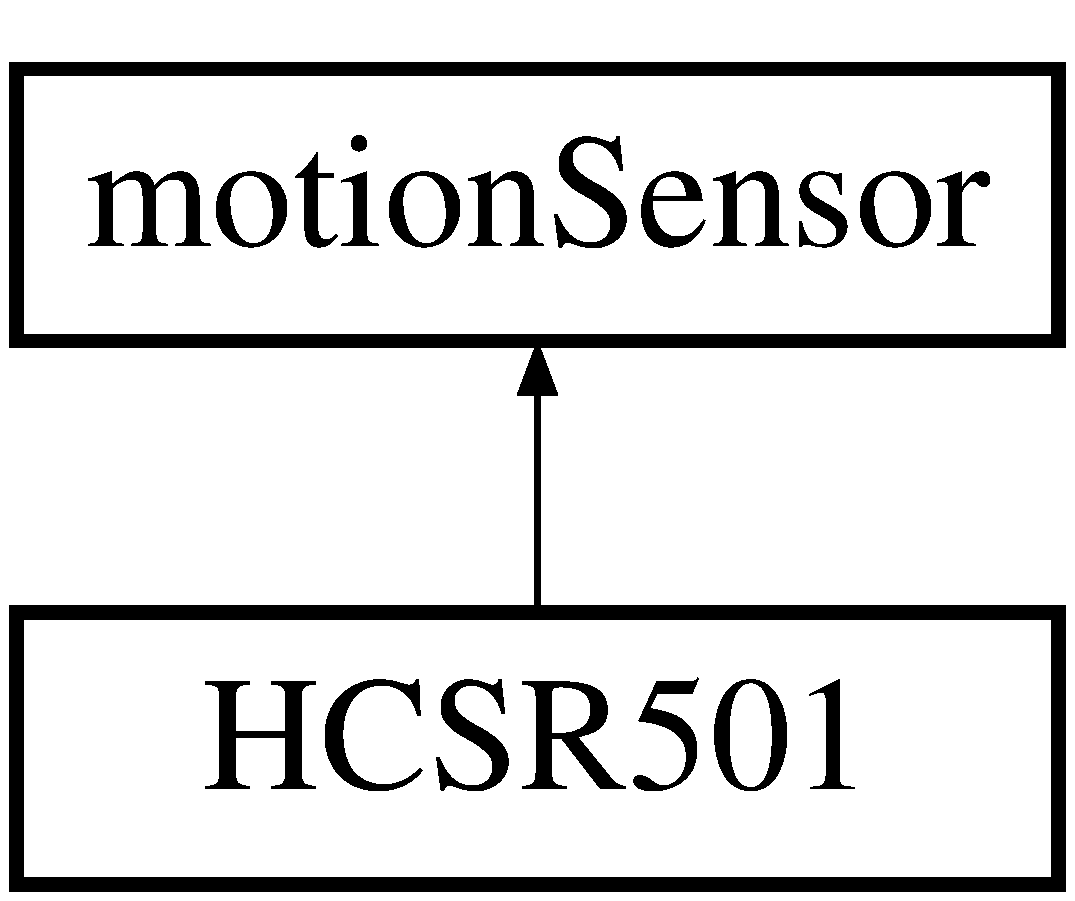
\includegraphics[height=2.000000cm]{classmotion_sensor}
\end{center}
\end{figure}
\subsection*{Public Member Functions}
\begin{DoxyCompactItemize}
\item 
virtual bool \mbox{\hyperlink{classmotion_sensor_a0b8701a41516d8b1140c39474b1db9db}{detect}} ()=0
\end{DoxyCompactItemize}


\subsection{Detailed Description}
A pure virtual class for a motion sensor chip like the \mbox{\hyperlink{class_h_c_s_r501}{H\+C\+S\+R501}}. 

This class is a pure virtual class. This means that you can access methods of the derived class when using reference or pointers. This makes the code easier to expand. \begin{DoxyWarning}{Warning}
T\+HE S\+O\+F\+T\+W\+A\+RE IS P\+R\+O\+V\+I\+D\+ED \char`\"{}\+A\+S I\+S\char`\"{}, W\+I\+T\+H\+O\+UT W\+A\+R\+R\+A\+N\+TY OF A\+NY K\+I\+ND. 
\end{DoxyWarning}


\subsection{Member Function Documentation}
\mbox{\Hypertarget{classmotion_sensor_a0b8701a41516d8b1140c39474b1db9db}\label{classmotion_sensor_a0b8701a41516d8b1140c39474b1db9db}} 
\index{motion\+Sensor@{motion\+Sensor}!detect@{detect}}
\index{detect@{detect}!motion\+Sensor@{motion\+Sensor}}
\subsubsection{\texorpdfstring{detect()}{detect()}}
{\footnotesize\ttfamily virtual bool motion\+Sensor\+::detect (\begin{DoxyParamCaption}{ }\end{DoxyParamCaption})\hspace{0.3cm}{\ttfamily [pure virtual]}}

detect whether there is anything is moving in the field of the motion sensor or not. \begin{DoxyReturn}{Returns}
A bool containing a 0 when nothing is detected and 1 when somthing is detected. 
\end{DoxyReturn}


Implemented in \mbox{\hyperlink{class_h_c_s_r501_a75456a573bf0066ee648f8f1a39d4966}{H\+C\+S\+R501}}.



The documentation for this class was generated from the following file\+:\begin{DoxyCompactItemize}
\item 
Demo/motion\+Sensor.\+hpp\end{DoxyCompactItemize}

\hypertarget{structpersonal_data}{}\section{personal\+Data Struct Reference}
\label{structpersonal_data}\index{personal\+Data@{personal\+Data}}
\subsection*{Public Attributes}
\begin{DoxyCompactItemize}
\item 
\mbox{\Hypertarget{structpersonal_data_abc1c669dbba62756cd53beab43cfd72d}\label{structpersonal_data_abc1c669dbba62756cd53beab43cfd72d}} 
char {\bfseries name} \mbox{[}255\mbox{]}
\item 
\mbox{\Hypertarget{structpersonal_data_a4ef7bb106614061624561a0c403ec223}\label{structpersonal_data_a4ef7bb106614061624561a0c403ec223}} 
uint8\+\_\+t {\bfseries access\+Level}
\item 
\mbox{\Hypertarget{structpersonal_data_a4c7d4c2a45f4e8f3295b094b8bc1da41}\label{structpersonal_data_a4c7d4c2a45f4e8f3295b094b8bc1da41}} 
uint8\+\_\+t {\bfseries U\+ID} \mbox{[}5\mbox{]}
\end{DoxyCompactItemize}


The documentation for this struct was generated from the following file\+:\begin{DoxyCompactItemize}
\item 
Demo/personal\+Data.\+hpp\end{DoxyCompactItemize}

\hypertarget{classreal_time_clock}{}\section{real\+Time\+Clock Class Reference}
\label{classreal_time_clock}\index{real\+Time\+Clock@{real\+Time\+Clock}}
Inheritance diagram for real\+Time\+Clock\+:\begin{figure}[H]
\begin{center}
\leavevmode
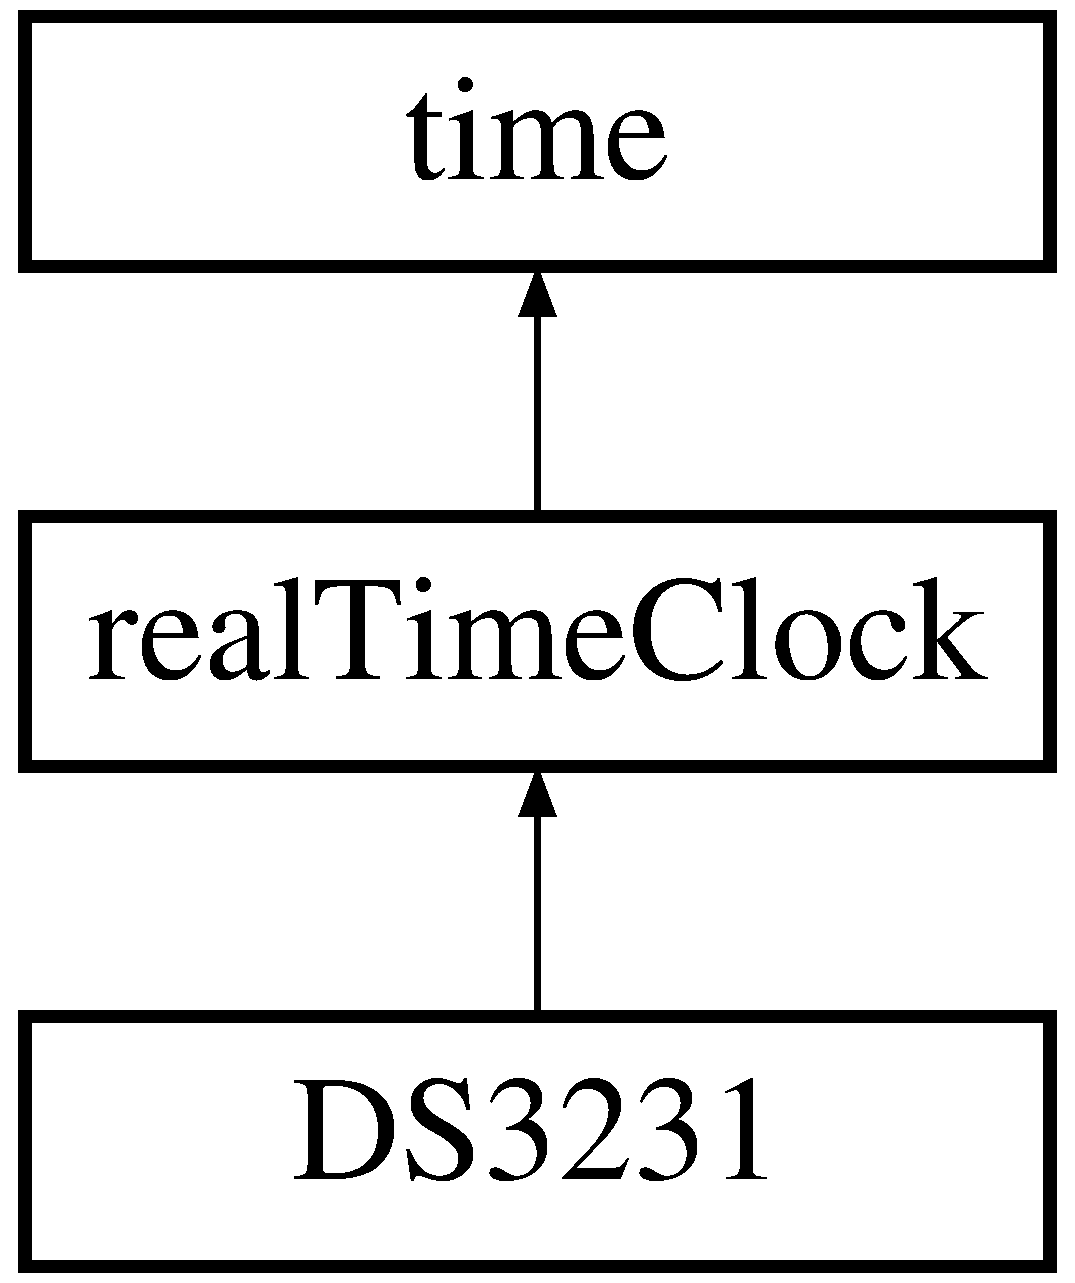
\includegraphics[height=3.000000cm]{classreal_time_clock}
\end{center}
\end{figure}
\subsection*{Public Member Functions}
\begin{DoxyCompactItemize}
\item 
virtual uint8\+\_\+t \mbox{\hyperlink{classreal_time_clock_a46bfe69dc650cc27e648ac7adb03afd0}{get\+Current\+Seconds}} ()=0
\begin{DoxyCompactList}\small\item\em Get the current value of the seconds register. \end{DoxyCompactList}\item 
virtual void \mbox{\hyperlink{classreal_time_clock_a463a64d4861c75e26a80712e1dd50e6b}{set\+Current\+Seconds}} (uint8\+\_\+t new\+Seconds)=0
\begin{DoxyCompactList}\small\item\em Set the current value in the seconds register. \end{DoxyCompactList}\item 
virtual uint8\+\_\+t \mbox{\hyperlink{classreal_time_clock_a8436f171be03d35a931004b3f3b144e9}{get\+Current\+Minutes}} ()=0
\begin{DoxyCompactList}\small\item\em Get the current value of the minutes register of the realtimeclock chip. \end{DoxyCompactList}\item 
virtual void \mbox{\hyperlink{classreal_time_clock_a52da7366cd5f1e4c270eb87e7298da42}{set\+Current\+Minutes}} (uint8\+\_\+t new\+Minutes)=0
\begin{DoxyCompactList}\small\item\em Set the current value in the minutes register. \end{DoxyCompactList}\item 
virtual uint8\+\_\+t \mbox{\hyperlink{classreal_time_clock_a2861a9bc75466a762b4cd8ce37193247}{get\+Current\+Hours}} ()=0
\begin{DoxyCompactList}\small\item\em Get the current value of the hours register. \end{DoxyCompactList}\item 
virtual void \mbox{\hyperlink{classreal_time_clock_a515d9de6067ae563bff5217da5100a23}{set\+Current\+Hours}} (uint8\+\_\+t new\+Hours)=0
\begin{DoxyCompactList}\small\item\em Set the current value in the hours register. \end{DoxyCompactList}\item 
virtual uint8\+\_\+t \mbox{\hyperlink{classreal_time_clock_a13b8ebc25275f183a1117402fc9e5e36}{get\+Current\+Day}} ()=0
\begin{DoxyCompactList}\small\item\em Get the current value in the day register. \end{DoxyCompactList}\item 
virtual void \mbox{\hyperlink{classreal_time_clock_a4a80a695cbb55860921f92509fae0cd0}{set\+Current\+Day}} (uint8\+\_\+t new\+Day)=0
\begin{DoxyCompactList}\small\item\em Set the current value in the day register. \end{DoxyCompactList}\item 
virtual uint8\+\_\+t \mbox{\hyperlink{classreal_time_clock_a910bce5ee911c18bd34a4154953ce2ac}{get\+Current\+Date}} ()=0
\begin{DoxyCompactList}\small\item\em Get the current value in the date register. \end{DoxyCompactList}\item 
virtual void \mbox{\hyperlink{classreal_time_clock_a7db563a518ae7b87ca6d77860906e517}{set\+Current\+Date}} (uint8\+\_\+t new\+Date)=0
\begin{DoxyCompactList}\small\item\em Set the current value in the date register. \end{DoxyCompactList}\item 
virtual uint8\+\_\+t \mbox{\hyperlink{classreal_time_clock_a24dd15babb345129fd995641946c5f2b}{get\+Current\+Month}} ()=0
\begin{DoxyCompactList}\small\item\em Get the current value in the month register. \end{DoxyCompactList}\item 
virtual void \mbox{\hyperlink{classreal_time_clock_a2edeb084630a78309bc574eceaf5d6ae}{set\+Current\+Month}} (uint8\+\_\+t new\+Month)=0
\begin{DoxyCompactList}\small\item\em Set the current value in the month register. \end{DoxyCompactList}\item 
virtual bool \mbox{\hyperlink{classreal_time_clock_ae0b15649f9135be8f0d9ada65084c28f}{get\+Current\+Century\+Bit}} ()=0
\begin{DoxyCompactList}\small\item\em Get the current century bit in the centrury register. \end{DoxyCompactList}\item 
virtual void \mbox{\hyperlink{classreal_time_clock_a50e19a6b0aef44719e91e3e753da0dce}{Reset\+Curent\+Century\+Bit}} ()=0
\begin{DoxyCompactList}\small\item\em Set the current value in the month register. \end{DoxyCompactList}\item 
virtual uint8\+\_\+t \mbox{\hyperlink{classreal_time_clock_a0cb99c34e2d6a089a62c8bea760c5add}{get\+Current\+Year}} ()=0
\begin{DoxyCompactList}\small\item\em Get the current value in the year register. \end{DoxyCompactList}\item 
virtual void \mbox{\hyperlink{classreal_time_clock_a4d6e8056f52cea52bab5c635c0860c12}{set\+Current\+Year}} (uint8\+\_\+t new\+Year)=0
\begin{DoxyCompactList}\small\item\em Set the current value in the year register. \end{DoxyCompactList}\item 
virtual void \mbox{\hyperlink{classreal_time_clock_a2d1613b3cd572f62bc9faaea6a0f82f2}{get\+Current\+Time\+Data}} (uint8\+\_\+t data\mbox{[}7\mbox{]})=0
\begin{DoxyCompactList}\small\item\em Get the current timestamp in an array. \end{DoxyCompactList}\item 
virtual \mbox{\hyperlink{classtimestamp}{timestamp}} \mbox{\hyperlink{classreal_time_clock_a08a7854ef9cef638996a267a953c9b14}{get\+Current\+Timestamp}} ()=0
\begin{DoxyCompactList}\small\item\em Get the a current timestamp /ref \mbox{\hyperlink{timestamp_8hpp_source}{timestamp.\+hpp}}. \end{DoxyCompactList}\item 
virtual void \mbox{\hyperlink{classreal_time_clock_aa7402c5941b089d4e86b2af20d48b7ba}{get\+Current\+Timestamp}} (\mbox{\hyperlink{classtimestamp}{timestamp}} \&ts)=0
\begin{DoxyCompactList}\small\item\em Update a existing timestamp. \end{DoxyCompactList}\item 
virtual uint8\+\_\+t \mbox{\hyperlink{classreal_time_clock_af4ff1775432a08af7e41db135d16bf65}{get\+Alarm\+One\+Seconds}} ()=0
\begin{DoxyCompactList}\small\item\em Get the value of the alarm one seconds register. \end{DoxyCompactList}\item 
virtual void \mbox{\hyperlink{classreal_time_clock_a448cbe8ab7f6649ee32eeb415721707f}{set\+Alarm\+One\+Seconds}} (uint8\+\_\+t new\+Seconds)=0
\begin{DoxyCompactList}\small\item\em Set a value in the alarm one seconds register. \end{DoxyCompactList}\item 
virtual uint8\+\_\+t \mbox{\hyperlink{classreal_time_clock_a0b3babca96f8246d4bb5e3ac2a95801d}{get\+Alarm\+Minutes}} (bool \mbox{\hyperlink{classalarm}{alarm}})=0
\begin{DoxyCompactList}\small\item\em Get the value of the alarm 1/2 minutes register. \end{DoxyCompactList}\item 
virtual void \mbox{\hyperlink{classreal_time_clock_a53ffba88cd87d05af58288fb4fc589b5}{set\+Alarm\+Minutes}} (bool \mbox{\hyperlink{classalarm}{alarm}}, uint8\+\_\+t new\+Minutes)=0
\begin{DoxyCompactList}\small\item\em Set a value in the alarm 1/2 minutes register. \end{DoxyCompactList}\item 
virtual uint8\+\_\+t \mbox{\hyperlink{classreal_time_clock_abca1ab557b357e3046d7d97eec89f750}{get\+Alarm\+Hours}} (bool \mbox{\hyperlink{classalarm}{alarm}})=0
\begin{DoxyCompactList}\small\item\em Get the value of the alarm 1/2 hours register. \end{DoxyCompactList}\item 
virtual void \mbox{\hyperlink{classreal_time_clock_a9f0cd64ce9a783f149fcbb9f7eb36524}{set\+Alarm\+Hours}} (bool \mbox{\hyperlink{classalarm}{alarm}}, uint8\+\_\+t new\+Hours)=0
\begin{DoxyCompactList}\small\item\em Set a value in the alarm 1/2 hours register. \end{DoxyCompactList}\item 
virtual uint8\+\_\+t \mbox{\hyperlink{classreal_time_clock_afe0a54cb2f803d01df03e2ea8e86bbf9}{get\+Alarm\+Day\+Date}} (bool \mbox{\hyperlink{classalarm}{alarm}})=0
\begin{DoxyCompactList}\small\item\em Get the value of the alarm 1/2 day and date register. \end{DoxyCompactList}\item 
virtual void \mbox{\hyperlink{classreal_time_clock_a2c2bb16a7fc59f463fb3aaed2fcd1926}{set\+Alarm\+Day\+Date}} (bool \mbox{\hyperlink{classalarm}{alarm}}, uint8\+\_\+t new\+Day\+Date)=0
\begin{DoxyCompactList}\small\item\em Set a value in the alarm 1/2 day and date register. \end{DoxyCompactList}\item 
virtual int16\+\_\+t \mbox{\hyperlink{classreal_time_clock_ac662348fcf7b5fb51fdcf79f83958a33}{get\+Current\+Temperature\+Celsius}} ()=0
\begin{DoxyCompactList}\small\item\em Get the current temperature in degrees celsius. \end{DoxyCompactList}\item 
virtual int16\+\_\+t \mbox{\hyperlink{classreal_time_clock_a8fe956100fc4e339cd68ab413465f666}{get\+Current\+Temperature\+Fahrenheit}} ()=0
\begin{DoxyCompactList}\small\item\em Get the current temperature in degrees fahrenheit. \end{DoxyCompactList}\item 
\mbox{\Hypertarget{classreal_time_clock_a13820319507d89a62a5b37b252ea6d0d}\label{classreal_time_clock_a13820319507d89a62a5b37b252ea6d0d}} 
virtual uint8\+\_\+t {\bfseries get\+Control\+Register} ()
\item 
\mbox{\Hypertarget{classreal_time_clock_ab4034ba75fb65a55fb725c37e89f7626}\label{classreal_time_clock_ab4034ba75fb65a55fb725c37e89f7626}} 
virtual void {\bfseries set\+Control\+Register} (uint8\+\_\+t new\+Byte)
\item 
\mbox{\Hypertarget{classreal_time_clock_a762441ffb1fbee666cd1642edfb8c929}\label{classreal_time_clock_a762441ffb1fbee666cd1642edfb8c929}} 
virtual bool {\bfseries get\+Control\+Register\+Bit} (uint8\+\_\+t bit\+Number)
\item 
\mbox{\Hypertarget{classreal_time_clock_af9b7db85f78d01060772bdb3b397ea3c}\label{classreal_time_clock_af9b7db85f78d01060772bdb3b397ea3c}} 
virtual void {\bfseries set\+Control\+Register\+Bit} (uint8\+\_\+t bit\+Number, bool new\+Bit)
\item 
\mbox{\Hypertarget{classreal_time_clock_a38dcc51b0b30a5e480ea7f18f2c792ba}\label{classreal_time_clock_a38dcc51b0b30a5e480ea7f18f2c792ba}} 
virtual uint8\+\_\+t {\bfseries get\+Status\+Register} ()=0
\item 
\mbox{\Hypertarget{classreal_time_clock_aa8ee80a7056c67543834508d0f04a218}\label{classreal_time_clock_aa8ee80a7056c67543834508d0f04a218}} 
virtual void {\bfseries set\+Status\+Register} (uint8\+\_\+t new\+Byte)=0
\item 
\mbox{\Hypertarget{classreal_time_clock_a2bc081385a6ad8273201d66217f8b2f0}\label{classreal_time_clock_a2bc081385a6ad8273201d66217f8b2f0}} 
virtual int8\+\_\+t {\bfseries get\+Aging\+Offset} ()=0
\item 
\mbox{\Hypertarget{classreal_time_clock_aacf97da86677ee3fb55b5180ba5c0727}\label{classreal_time_clock_aacf97da86677ee3fb55b5180ba5c0727}} 
virtual void {\bfseries set\+Aging\+Offset} (int8\+\_\+t new\+Aging\+Offset)=0
\item 
\mbox{\Hypertarget{classreal_time_clock_afb5132ca3cbe80552a88041cead0a2b3}\label{classreal_time_clock_afb5132ca3cbe80552a88041cead0a2b3}} 
virtual void {\bfseries update} ()=0
\end{DoxyCompactItemize}
\subsection*{Additional Inherited Members}


\subsection{Member Function Documentation}
\mbox{\Hypertarget{classreal_time_clock_afe0a54cb2f803d01df03e2ea8e86bbf9}\label{classreal_time_clock_afe0a54cb2f803d01df03e2ea8e86bbf9}} 
\index{real\+Time\+Clock@{real\+Time\+Clock}!get\+Alarm\+Day\+Date@{get\+Alarm\+Day\+Date}}
\index{get\+Alarm\+Day\+Date@{get\+Alarm\+Day\+Date}!real\+Time\+Clock@{real\+Time\+Clock}}
\subsubsection{\texorpdfstring{get\+Alarm\+Day\+Date()}{getAlarmDayDate()}}
{\footnotesize\ttfamily virtual uint8\+\_\+t real\+Time\+Clock\+::get\+Alarm\+Day\+Date (\begin{DoxyParamCaption}\item[{bool}]{alarm }\end{DoxyParamCaption})\hspace{0.3cm}{\ttfamily [pure virtual]}}



Get the value of the alarm 1/2 day and date register. 


\begin{DoxyParams}{Parameters}
{\em alarm} & The alarm you want the value of (0 or 1). \\
\hline
\end{DoxyParams}
\begin{DoxyReturn}{Returns}
An uint8\+\_\+t containing the current value in alarm 1/2 day and date register.
\end{DoxyReturn}
This method will get you the current value of the any alarm day and date register. You can choose which alarm register using the parameter alarm. 0 = alarm one, 1 = alarm two. \begin{DoxyWarning}{Warning}
note that the paramether is a boolean. Therefore alarm one = 0 and alarm two = 1. 
\end{DoxyWarning}


Implemented in \mbox{\hyperlink{class_d_s3231_a0b013c68f96b5145c1c9feb9270855a7}{D\+S3231}}.

\mbox{\Hypertarget{classreal_time_clock_abca1ab557b357e3046d7d97eec89f750}\label{classreal_time_clock_abca1ab557b357e3046d7d97eec89f750}} 
\index{real\+Time\+Clock@{real\+Time\+Clock}!get\+Alarm\+Hours@{get\+Alarm\+Hours}}
\index{get\+Alarm\+Hours@{get\+Alarm\+Hours}!real\+Time\+Clock@{real\+Time\+Clock}}
\subsubsection{\texorpdfstring{get\+Alarm\+Hours()}{getAlarmHours()}}
{\footnotesize\ttfamily virtual uint8\+\_\+t real\+Time\+Clock\+::get\+Alarm\+Hours (\begin{DoxyParamCaption}\item[{bool}]{alarm }\end{DoxyParamCaption})\hspace{0.3cm}{\ttfamily [pure virtual]}}



Get the value of the alarm 1/2 hours register. 


\begin{DoxyParams}{Parameters}
{\em alarm} & The alarm you want the value of (0 or 1). \\
\hline
\end{DoxyParams}
\begin{DoxyReturn}{Returns}
An uint8\+\_\+t containing the current value in alarm 1/2 hours register.
\end{DoxyReturn}
This method will get you the current value of the any alarm hours register. You can choose which alarm register using the parameter alarm. 0 = alarm one, 1 = alarm two. \begin{DoxyWarning}{Warning}
note that the paramether is a boolean. Therefore alarm one = 0 and alarm two = 1. 
\end{DoxyWarning}


Implemented in \mbox{\hyperlink{class_d_s3231_a8dc2f4546600209d16f109764c2f4434}{D\+S3231}}.

\mbox{\Hypertarget{classreal_time_clock_a0b3babca96f8246d4bb5e3ac2a95801d}\label{classreal_time_clock_a0b3babca96f8246d4bb5e3ac2a95801d}} 
\index{real\+Time\+Clock@{real\+Time\+Clock}!get\+Alarm\+Minutes@{get\+Alarm\+Minutes}}
\index{get\+Alarm\+Minutes@{get\+Alarm\+Minutes}!real\+Time\+Clock@{real\+Time\+Clock}}
\subsubsection{\texorpdfstring{get\+Alarm\+Minutes()}{getAlarmMinutes()}}
{\footnotesize\ttfamily virtual uint8\+\_\+t real\+Time\+Clock\+::get\+Alarm\+Minutes (\begin{DoxyParamCaption}\item[{bool}]{alarm }\end{DoxyParamCaption})\hspace{0.3cm}{\ttfamily [pure virtual]}}



Get the value of the alarm 1/2 minutes register. 


\begin{DoxyParams}{Parameters}
{\em alarm} & The alarm you want the value of (0 or 1). \\
\hline
\end{DoxyParams}
\begin{DoxyReturn}{Returns}
An uint8\+\_\+t containing the current value in alarm 1/2 minutes register.
\end{DoxyReturn}
This method will get you the current value of the any alarm minutes register. You can choose which alarm register using the parameter alarm. 0 = alarm one, 1 = alarm two. \begin{DoxyWarning}{Warning}
note that the paramether is a boolean. Therefore alarm one = 0 and alarm two = 1. 
\end{DoxyWarning}


Implemented in \mbox{\hyperlink{class_d_s3231_ae11a0dcc34e9c8a9b875989172339957}{D\+S3231}}.

\mbox{\Hypertarget{classreal_time_clock_af4ff1775432a08af7e41db135d16bf65}\label{classreal_time_clock_af4ff1775432a08af7e41db135d16bf65}} 
\index{real\+Time\+Clock@{real\+Time\+Clock}!get\+Alarm\+One\+Seconds@{get\+Alarm\+One\+Seconds}}
\index{get\+Alarm\+One\+Seconds@{get\+Alarm\+One\+Seconds}!real\+Time\+Clock@{real\+Time\+Clock}}
\subsubsection{\texorpdfstring{get\+Alarm\+One\+Seconds()}{getAlarmOneSeconds()}}
{\footnotesize\ttfamily virtual uint8\+\_\+t real\+Time\+Clock\+::get\+Alarm\+One\+Seconds (\begin{DoxyParamCaption}{ }\end{DoxyParamCaption})\hspace{0.3cm}{\ttfamily [pure virtual]}}



Get the value of the alarm one seconds register. 

\begin{DoxyReturn}{Returns}
An uint8\+\_\+t containing the current value in alarm 1 seconds register. 
\end{DoxyReturn}


Implemented in \mbox{\hyperlink{class_d_s3231_afd2b16482de8abc10981fdfca0e181a6}{D\+S3231}}.

\mbox{\Hypertarget{classreal_time_clock_ae0b15649f9135be8f0d9ada65084c28f}\label{classreal_time_clock_ae0b15649f9135be8f0d9ada65084c28f}} 
\index{real\+Time\+Clock@{real\+Time\+Clock}!get\+Current\+Century\+Bit@{get\+Current\+Century\+Bit}}
\index{get\+Current\+Century\+Bit@{get\+Current\+Century\+Bit}!real\+Time\+Clock@{real\+Time\+Clock}}
\subsubsection{\texorpdfstring{get\+Current\+Century\+Bit()}{getCurrentCenturyBit()}}
{\footnotesize\ttfamily virtual bool real\+Time\+Clock\+::get\+Current\+Century\+Bit (\begin{DoxyParamCaption}{ }\end{DoxyParamCaption})\hspace{0.3cm}{\ttfamily [pure virtual]}}



Get the current century bit in the centrury register. 

\begin{DoxyReturn}{Returns}
A bool that contains the current value of the month register. (0 or 1) 
\end{DoxyReturn}


Implemented in \mbox{\hyperlink{class_d_s3231_a38dfc1567d3419d5aeecd2062d4121c7}{D\+S3231}}.

\mbox{\Hypertarget{classreal_time_clock_a910bce5ee911c18bd34a4154953ce2ac}\label{classreal_time_clock_a910bce5ee911c18bd34a4154953ce2ac}} 
\index{real\+Time\+Clock@{real\+Time\+Clock}!get\+Current\+Date@{get\+Current\+Date}}
\index{get\+Current\+Date@{get\+Current\+Date}!real\+Time\+Clock@{real\+Time\+Clock}}
\subsubsection{\texorpdfstring{get\+Current\+Date()}{getCurrentDate()}}
{\footnotesize\ttfamily virtual uint8\+\_\+t real\+Time\+Clock\+::get\+Current\+Date (\begin{DoxyParamCaption}{ }\end{DoxyParamCaption})\hspace{0.3cm}{\ttfamily [pure virtual]}}



Get the current value in the date register. 

\begin{DoxyReturn}{Returns}
An uint8\+\_\+t that contains the current value of the date register. (1 -\/ $\sim$31) 
\end{DoxyReturn}


Implemented in \mbox{\hyperlink{class_d_s3231_a346341a4d3c6615103b33fbff7a12884}{D\+S3231}}.

\mbox{\Hypertarget{classreal_time_clock_a13b8ebc25275f183a1117402fc9e5e36}\label{classreal_time_clock_a13b8ebc25275f183a1117402fc9e5e36}} 
\index{real\+Time\+Clock@{real\+Time\+Clock}!get\+Current\+Day@{get\+Current\+Day}}
\index{get\+Current\+Day@{get\+Current\+Day}!real\+Time\+Clock@{real\+Time\+Clock}}
\subsubsection{\texorpdfstring{get\+Current\+Day()}{getCurrentDay()}}
{\footnotesize\ttfamily virtual uint8\+\_\+t real\+Time\+Clock\+::get\+Current\+Day (\begin{DoxyParamCaption}{ }\end{DoxyParamCaption})\hspace{0.3cm}{\ttfamily [pure virtual]}}



Get the current value in the day register. 

\begin{DoxyReturn}{Returns}
An uint8\+\_\+t that contains the current value of the day register of the realtimeclock chip. (1 = monday 7 == sunday) 
\end{DoxyReturn}


Implemented in \mbox{\hyperlink{class_d_s3231_a813bbe55a08e1911d498511795721477}{D\+S3231}}.

\mbox{\Hypertarget{classreal_time_clock_a2861a9bc75466a762b4cd8ce37193247}\label{classreal_time_clock_a2861a9bc75466a762b4cd8ce37193247}} 
\index{real\+Time\+Clock@{real\+Time\+Clock}!get\+Current\+Hours@{get\+Current\+Hours}}
\index{get\+Current\+Hours@{get\+Current\+Hours}!real\+Time\+Clock@{real\+Time\+Clock}}
\subsubsection{\texorpdfstring{get\+Current\+Hours()}{getCurrentHours()}}
{\footnotesize\ttfamily virtual uint8\+\_\+t real\+Time\+Clock\+::get\+Current\+Hours (\begin{DoxyParamCaption}{ }\end{DoxyParamCaption})\hspace{0.3cm}{\ttfamily [pure virtual]}}



Get the current value of the hours register. 

\begin{DoxyReturn}{Returns}
An uint8\+\_\+t that contains the current value of the hours register. (0 -\/ 23) 
\end{DoxyReturn}


Implemented in \mbox{\hyperlink{class_d_s3231_a019d8ed8074a02937c0777424be3d0ae}{D\+S3231}}.

\mbox{\Hypertarget{classreal_time_clock_a8436f171be03d35a931004b3f3b144e9}\label{classreal_time_clock_a8436f171be03d35a931004b3f3b144e9}} 
\index{real\+Time\+Clock@{real\+Time\+Clock}!get\+Current\+Minutes@{get\+Current\+Minutes}}
\index{get\+Current\+Minutes@{get\+Current\+Minutes}!real\+Time\+Clock@{real\+Time\+Clock}}
\subsubsection{\texorpdfstring{get\+Current\+Minutes()}{getCurrentMinutes()}}
{\footnotesize\ttfamily virtual uint8\+\_\+t real\+Time\+Clock\+::get\+Current\+Minutes (\begin{DoxyParamCaption}{ }\end{DoxyParamCaption})\hspace{0.3cm}{\ttfamily [pure virtual]}}



Get the current value of the minutes register of the realtimeclock chip. 

\begin{DoxyReturn}{Returns}
An uint8\+\_\+t that contains the current value of the minutes register. (0 -\/ 59) 
\end{DoxyReturn}


Implemented in \mbox{\hyperlink{class_d_s3231_a08f384e1897214d4a201aaaecde3b8a4}{D\+S3231}}.

\mbox{\Hypertarget{classreal_time_clock_a24dd15babb345129fd995641946c5f2b}\label{classreal_time_clock_a24dd15babb345129fd995641946c5f2b}} 
\index{real\+Time\+Clock@{real\+Time\+Clock}!get\+Current\+Month@{get\+Current\+Month}}
\index{get\+Current\+Month@{get\+Current\+Month}!real\+Time\+Clock@{real\+Time\+Clock}}
\subsubsection{\texorpdfstring{get\+Current\+Month()}{getCurrentMonth()}}
{\footnotesize\ttfamily virtual uint8\+\_\+t real\+Time\+Clock\+::get\+Current\+Month (\begin{DoxyParamCaption}{ }\end{DoxyParamCaption})\hspace{0.3cm}{\ttfamily [pure virtual]}}



Get the current value in the month register. 

\begin{DoxyReturn}{Returns}
A uint8\+\_\+t that contains the current value of the month register. (1 -\/ 12) 
\end{DoxyReturn}


Implemented in \mbox{\hyperlink{class_d_s3231_a8d7a965802afacc16b4d5af86e0ed11e}{D\+S3231}}.

\mbox{\Hypertarget{classreal_time_clock_a46bfe69dc650cc27e648ac7adb03afd0}\label{classreal_time_clock_a46bfe69dc650cc27e648ac7adb03afd0}} 
\index{real\+Time\+Clock@{real\+Time\+Clock}!get\+Current\+Seconds@{get\+Current\+Seconds}}
\index{get\+Current\+Seconds@{get\+Current\+Seconds}!real\+Time\+Clock@{real\+Time\+Clock}}
\subsubsection{\texorpdfstring{get\+Current\+Seconds()}{getCurrentSeconds()}}
{\footnotesize\ttfamily virtual uint8\+\_\+t real\+Time\+Clock\+::get\+Current\+Seconds (\begin{DoxyParamCaption}{ }\end{DoxyParamCaption})\hspace{0.3cm}{\ttfamily [pure virtual]}}



Get the current value of the seconds register. 

\begin{DoxyReturn}{Returns}
An uint8\+\_\+t that contains the current value of the seconds register. (0 -\/ 59) 
\end{DoxyReturn}


Implemented in \mbox{\hyperlink{class_d_s3231_a8a5357eae07991d94f8f7610a3f3073a}{D\+S3231}}.

\mbox{\Hypertarget{classreal_time_clock_ac662348fcf7b5fb51fdcf79f83958a33}\label{classreal_time_clock_ac662348fcf7b5fb51fdcf79f83958a33}} 
\index{real\+Time\+Clock@{real\+Time\+Clock}!get\+Current\+Temperature\+Celsius@{get\+Current\+Temperature\+Celsius}}
\index{get\+Current\+Temperature\+Celsius@{get\+Current\+Temperature\+Celsius}!real\+Time\+Clock@{real\+Time\+Clock}}
\subsubsection{\texorpdfstring{get\+Current\+Temperature\+Celsius()}{getCurrentTemperatureCelsius()}}
{\footnotesize\ttfamily virtual int16\+\_\+t real\+Time\+Clock\+::get\+Current\+Temperature\+Celsius (\begin{DoxyParamCaption}{ }\end{DoxyParamCaption})\hspace{0.3cm}{\ttfamily [pure virtual]}}



Get the current temperature in degrees celsius. 

\begin{DoxyReturn}{Returns}
An int16\+\_\+t containing the current temperature in degrees celsius.
\end{DoxyReturn}
Note that it is a int16\+\_\+t, this means that the value IS N\+OT be a floating point number. Most chips will support a floating point number. But it\textquotesingle{}s not very smart to use those because of the small computer we are using (Arduino due). The floating point numbers are in my opinion not really needed to display a accurate temperature. 

Implemented in \mbox{\hyperlink{class_d_s3231_abd46c1cf5f5c78e3222c3677e70a1272}{D\+S3231}}.

\mbox{\Hypertarget{classreal_time_clock_a8fe956100fc4e339cd68ab413465f666}\label{classreal_time_clock_a8fe956100fc4e339cd68ab413465f666}} 
\index{real\+Time\+Clock@{real\+Time\+Clock}!get\+Current\+Temperature\+Fahrenheit@{get\+Current\+Temperature\+Fahrenheit}}
\index{get\+Current\+Temperature\+Fahrenheit@{get\+Current\+Temperature\+Fahrenheit}!real\+Time\+Clock@{real\+Time\+Clock}}
\subsubsection{\texorpdfstring{get\+Current\+Temperature\+Fahrenheit()}{getCurrentTemperatureFahrenheit()}}
{\footnotesize\ttfamily virtual int16\+\_\+t real\+Time\+Clock\+::get\+Current\+Temperature\+Fahrenheit (\begin{DoxyParamCaption}{ }\end{DoxyParamCaption})\hspace{0.3cm}{\ttfamily [pure virtual]}}



Get the current temperature in degrees fahrenheit. 

\begin{DoxyReturn}{Returns}
An int16\+\_\+t containing the current temperature in degrees farhenheit.
\end{DoxyReturn}
Note that it is a int16\+\_\+t, this means that the value IS N\+OT be a floating point number. Most chips will support a floating point number. But it\textquotesingle{}s not very smart to use those because of the small computer we are using (Arduino due). The floating point numbers are in my opinion not really needed to display a accurate temperature. The used formula for correct convertion can be found here\+: \href{https://www.rapidtables.com/convert/temperature/how-celsius-to-fahrenheit.html}{\tt Celcius to Farhenheit formula} 

Implemented in \mbox{\hyperlink{class_d_s3231_aa31acb133cc63aa7a2a25eda6244c9df}{D\+S3231}}.

\mbox{\Hypertarget{classreal_time_clock_a2d1613b3cd572f62bc9faaea6a0f82f2}\label{classreal_time_clock_a2d1613b3cd572f62bc9faaea6a0f82f2}} 
\index{real\+Time\+Clock@{real\+Time\+Clock}!get\+Current\+Time\+Data@{get\+Current\+Time\+Data}}
\index{get\+Current\+Time\+Data@{get\+Current\+Time\+Data}!real\+Time\+Clock@{real\+Time\+Clock}}
\subsubsection{\texorpdfstring{get\+Current\+Time\+Data()}{getCurrentTimeData()}}
{\footnotesize\ttfamily virtual void real\+Time\+Clock\+::get\+Current\+Time\+Data (\begin{DoxyParamCaption}\item[{uint8\+\_\+t}]{data\mbox{[}7\mbox{]} }\end{DoxyParamCaption})\hspace{0.3cm}{\ttfamily [pure virtual]}}



Get the current timestamp in an array. 


\begin{DoxyParams}{Parameters}
{\em data\mbox{[}7\mbox{]}} & is a pointer to an array where the current timestamp will be stored in.\\
\hline
\end{DoxyParams}
This method returns a array with raw data (B\+CD values) of the following registers\+: array\mbox{[}0\mbox{]} = seconds array\mbox{[}1\mbox{]} = minutes array\mbox{[}2\mbox{]} = hours array\mbox{[}3\mbox{]} = day array\mbox{[}4\mbox{]} = date array\mbox{[}5\mbox{]} = month array\mbox{[}6\mbox{]} = year array\mbox{[}7\mbox{]} = century (/ref \mbox{\hyperlink{time_8hpp_source}{time.\+hpp}} current\+Century) \begin{DoxyWarning}{Warning}
The array will be filled with raw data. Most registers are B\+CD register. This means that the decimal value might not be what you expected. 

Note that the array must have a size of 7. All the data in the array will be overritten. 
\end{DoxyWarning}


Implemented in \mbox{\hyperlink{class_d_s3231_a0ca41c2242367c5ff1424d1b12f909c5}{D\+S3231}}.

\mbox{\Hypertarget{classreal_time_clock_a08a7854ef9cef638996a267a953c9b14}\label{classreal_time_clock_a08a7854ef9cef638996a267a953c9b14}} 
\index{real\+Time\+Clock@{real\+Time\+Clock}!get\+Current\+Timestamp@{get\+Current\+Timestamp}}
\index{get\+Current\+Timestamp@{get\+Current\+Timestamp}!real\+Time\+Clock@{real\+Time\+Clock}}
\subsubsection{\texorpdfstring{get\+Current\+Timestamp()}{getCurrentTimestamp()}\hspace{0.1cm}{\footnotesize\ttfamily [1/2]}}
{\footnotesize\ttfamily virtual \mbox{\hyperlink{classtimestamp}{timestamp}} real\+Time\+Clock\+::get\+Current\+Timestamp (\begin{DoxyParamCaption}{ }\end{DoxyParamCaption})\hspace{0.3cm}{\ttfamily [pure virtual]}}



Get the a current timestamp /ref \mbox{\hyperlink{timestamp_8hpp_source}{timestamp.\+hpp}}. 

\begin{DoxyReturn}{Returns}
a timestamp with the containing the current time.
\end{DoxyReturn}
This method returns a timestamp with the same data as \mbox{\hyperlink{classreal_time_clock_a2d1613b3cd572f62bc9faaea6a0f82f2}{get\+Current\+Time\+Data}}. You might want to use this over \mbox{\hyperlink{classreal_time_clock_a2d1613b3cd572f62bc9faaea6a0f82f2}{get\+Current\+Time\+Data}} because there is extra functionality in the timestamp class. Look at /ref \mbox{\hyperlink{timestamp_8hpp_source}{timestamp.\+hpp}} for further information about the timestamp format. 

Implemented in \mbox{\hyperlink{class_d_s3231_a04e087a918d2d48b0cdd2e3c6c2f595f}{D\+S3231}}.

\mbox{\Hypertarget{classreal_time_clock_aa7402c5941b089d4e86b2af20d48b7ba}\label{classreal_time_clock_aa7402c5941b089d4e86b2af20d48b7ba}} 
\index{real\+Time\+Clock@{real\+Time\+Clock}!get\+Current\+Timestamp@{get\+Current\+Timestamp}}
\index{get\+Current\+Timestamp@{get\+Current\+Timestamp}!real\+Time\+Clock@{real\+Time\+Clock}}
\subsubsection{\texorpdfstring{get\+Current\+Timestamp()}{getCurrentTimestamp()}\hspace{0.1cm}{\footnotesize\ttfamily [2/2]}}
{\footnotesize\ttfamily virtual void real\+Time\+Clock\+::get\+Current\+Timestamp (\begin{DoxyParamCaption}\item[{\mbox{\hyperlink{classtimestamp}{timestamp}} \&}]{ts }\end{DoxyParamCaption})\hspace{0.3cm}{\ttfamily [pure virtual]}}



Update a existing timestamp. 


\begin{DoxyParams}{Parameters}
{\em ts} & the timestamp you want to update.\\
\hline
\end{DoxyParams}
This method will change the given timestamp ts its value to the current time. \begin{DoxyWarning}{Warning}
The given timestamp ts will be changed when this method is executed. 
\end{DoxyWarning}


Implemented in \mbox{\hyperlink{class_d_s3231_ad94d54ed265fb5b911b4281f0103b0b0}{D\+S3231}}.

\mbox{\Hypertarget{classreal_time_clock_a0cb99c34e2d6a089a62c8bea760c5add}\label{classreal_time_clock_a0cb99c34e2d6a089a62c8bea760c5add}} 
\index{real\+Time\+Clock@{real\+Time\+Clock}!get\+Current\+Year@{get\+Current\+Year}}
\index{get\+Current\+Year@{get\+Current\+Year}!real\+Time\+Clock@{real\+Time\+Clock}}
\subsubsection{\texorpdfstring{get\+Current\+Year()}{getCurrentYear()}}
{\footnotesize\ttfamily virtual uint8\+\_\+t real\+Time\+Clock\+::get\+Current\+Year (\begin{DoxyParamCaption}{ }\end{DoxyParamCaption})\hspace{0.3cm}{\ttfamily [pure virtual]}}



Get the current value in the year register. 

\begin{DoxyReturn}{Returns}
A uin8\+\_\+t containing the current value of the year register (0 -\/ 99) 
\end{DoxyReturn}
\begin{DoxyWarning}{Warning}
Most chips will set the century bit when the year register went past 99. Note when the century bit is high you\textquotesingle{}re in a new century. \#update will automaticly update the current century in \mbox{\hyperlink{time_8hpp_source}{time.\+hpp}} and reset the century bit. 
\end{DoxyWarning}


Implemented in \mbox{\hyperlink{class_d_s3231_a28a340b10b045ad1e8b94532a57c3759}{D\+S3231}}.

\mbox{\Hypertarget{classreal_time_clock_a50e19a6b0aef44719e91e3e753da0dce}\label{classreal_time_clock_a50e19a6b0aef44719e91e3e753da0dce}} 
\index{real\+Time\+Clock@{real\+Time\+Clock}!Reset\+Curent\+Century\+Bit@{Reset\+Curent\+Century\+Bit}}
\index{Reset\+Curent\+Century\+Bit@{Reset\+Curent\+Century\+Bit}!real\+Time\+Clock@{real\+Time\+Clock}}
\subsubsection{\texorpdfstring{Reset\+Curent\+Century\+Bit()}{ResetCurentCenturyBit()}}
{\footnotesize\ttfamily virtual void real\+Time\+Clock\+::\+Reset\+Curent\+Century\+Bit (\begin{DoxyParamCaption}{ }\end{DoxyParamCaption})\hspace{0.3cm}{\ttfamily [pure virtual]}}



Set the current value in the month register. 


\begin{DoxyParams}{Parameters}
{\em new\+Month} & the value you want to set into the month register. (1 -\/ 12)\\
\hline
\end{DoxyParams}
The current\+Century in \mbox{\hyperlink{time_8hpp_source}{time.\+hpp}} will automaticly be updated after this bit was high when you call update. \begin{DoxyWarning}{Warning}
This method will override the current value in the month register. 

Only use this function if you know what you\textquotesingle{}re doing. The current\+Century in \mbox{\hyperlink{time_8hpp_source}{time.\+hpp}} will automaticly be updated after this bit was high when you call \#update. 
\end{DoxyWarning}


Implemented in \mbox{\hyperlink{class_d_s3231_a6477bd1bb91d3df6a088c369692f46a3}{D\+S3231}}.

\mbox{\Hypertarget{classreal_time_clock_a2c2bb16a7fc59f463fb3aaed2fcd1926}\label{classreal_time_clock_a2c2bb16a7fc59f463fb3aaed2fcd1926}} 
\index{real\+Time\+Clock@{real\+Time\+Clock}!set\+Alarm\+Day\+Date@{set\+Alarm\+Day\+Date}}
\index{set\+Alarm\+Day\+Date@{set\+Alarm\+Day\+Date}!real\+Time\+Clock@{real\+Time\+Clock}}
\subsubsection{\texorpdfstring{set\+Alarm\+Day\+Date()}{setAlarmDayDate()}}
{\footnotesize\ttfamily virtual void real\+Time\+Clock\+::set\+Alarm\+Day\+Date (\begin{DoxyParamCaption}\item[{bool}]{alarm,  }\item[{uint8\+\_\+t}]{new\+Day\+Date }\end{DoxyParamCaption})\hspace{0.3cm}{\ttfamily [pure virtual]}}



Set a value in the alarm 1/2 day and date register. 


\begin{DoxyParams}{Parameters}
{\em alarm} & The alarm you want the value of (0 or 1). \\
\hline
{\em new\+Day\+Date} & The value you want to store in the alarm 1/2 day and date register.\\
\hline
\end{DoxyParams}
This method will set a new value into the chosen alarm day and date register. You can choose which alarm register using the parameter alarm. 0 = alarm one, 1 = alarm two. \begin{DoxyWarning}{Warning}
note that the paramether is a boolean. Therefore alarm one = 0 and alarm two = 1. 

the value in the chosen alarm day and date register will change. 
\end{DoxyWarning}


Implemented in \mbox{\hyperlink{class_d_s3231_aa2048cc766ca58f707e84cbc564c1276}{D\+S3231}}.

\mbox{\Hypertarget{classreal_time_clock_a9f0cd64ce9a783f149fcbb9f7eb36524}\label{classreal_time_clock_a9f0cd64ce9a783f149fcbb9f7eb36524}} 
\index{real\+Time\+Clock@{real\+Time\+Clock}!set\+Alarm\+Hours@{set\+Alarm\+Hours}}
\index{set\+Alarm\+Hours@{set\+Alarm\+Hours}!real\+Time\+Clock@{real\+Time\+Clock}}
\subsubsection{\texorpdfstring{set\+Alarm\+Hours()}{setAlarmHours()}}
{\footnotesize\ttfamily virtual void real\+Time\+Clock\+::set\+Alarm\+Hours (\begin{DoxyParamCaption}\item[{bool}]{alarm,  }\item[{uint8\+\_\+t}]{new\+Hours }\end{DoxyParamCaption})\hspace{0.3cm}{\ttfamily [pure virtual]}}



Set a value in the alarm 1/2 hours register. 


\begin{DoxyParams}{Parameters}
{\em alarm} & The alarm you want the value of (0 or 1). \\
\hline
{\em new\+Hours} & The value you want to store in the alarm 1/2 register.\\
\hline
\end{DoxyParams}
This method will set a new value into the chosen alarm hours register. You can choose which alarm register using the parameter alarm. 0 = alarm one, 1 = alarm two. \begin{DoxyWarning}{Warning}
note that the paramether is a boolean. Therefore alarm one = 0 and alarm two = 1. 

the value in the chosen alarm hours register will change. 
\end{DoxyWarning}


Implemented in \mbox{\hyperlink{class_d_s3231_a0bcc7e2285869ffbe29d19c593f5a447}{D\+S3231}}.

\mbox{\Hypertarget{classreal_time_clock_a53ffba88cd87d05af58288fb4fc589b5}\label{classreal_time_clock_a53ffba88cd87d05af58288fb4fc589b5}} 
\index{real\+Time\+Clock@{real\+Time\+Clock}!set\+Alarm\+Minutes@{set\+Alarm\+Minutes}}
\index{set\+Alarm\+Minutes@{set\+Alarm\+Minutes}!real\+Time\+Clock@{real\+Time\+Clock}}
\subsubsection{\texorpdfstring{set\+Alarm\+Minutes()}{setAlarmMinutes()}}
{\footnotesize\ttfamily virtual void real\+Time\+Clock\+::set\+Alarm\+Minutes (\begin{DoxyParamCaption}\item[{bool}]{alarm,  }\item[{uint8\+\_\+t}]{new\+Minutes }\end{DoxyParamCaption})\hspace{0.3cm}{\ttfamily [pure virtual]}}



Set a value in the alarm 1/2 minutes register. 


\begin{DoxyParams}{Parameters}
{\em alarm} & The alarm you want the value of (0 or 1). \\
\hline
{\em new\+Minutes} & The value you want to store in the alarm 1/2 register.\\
\hline
\end{DoxyParams}
This method will set a new value into the chosen alarm minutes register. You can choose which alarm register using the parameter alarm. 0 = alarm one, 1 = alarm two. \begin{DoxyWarning}{Warning}
note that the paramether is a boolean. Therefore alarm one = 0 and alarm two = 1. 

the value in the chosen alarm minutes register will change. 
\end{DoxyWarning}


Implemented in \mbox{\hyperlink{class_d_s3231_a9c1f5b183c24f3062c1c8c299f46023c}{D\+S3231}}.

\mbox{\Hypertarget{classreal_time_clock_a448cbe8ab7f6649ee32eeb415721707f}\label{classreal_time_clock_a448cbe8ab7f6649ee32eeb415721707f}} 
\index{real\+Time\+Clock@{real\+Time\+Clock}!set\+Alarm\+One\+Seconds@{set\+Alarm\+One\+Seconds}}
\index{set\+Alarm\+One\+Seconds@{set\+Alarm\+One\+Seconds}!real\+Time\+Clock@{real\+Time\+Clock}}
\subsubsection{\texorpdfstring{set\+Alarm\+One\+Seconds()}{setAlarmOneSeconds()}}
{\footnotesize\ttfamily virtual void real\+Time\+Clock\+::set\+Alarm\+One\+Seconds (\begin{DoxyParamCaption}\item[{uint8\+\_\+t}]{new\+Seconds }\end{DoxyParamCaption})\hspace{0.3cm}{\ttfamily [pure virtual]}}



Set a value in the alarm one seconds register. 


\begin{DoxyParams}{Parameters}
{\em new\+Seconds} & The value you want to store in the alarm 1 seconds register. \\
\hline
\end{DoxyParams}
\begin{DoxyWarning}{Warning}
The value in the alarm one seconds register will change. 
\end{DoxyWarning}


Implemented in \mbox{\hyperlink{class_d_s3231_ae294f3c8c8634a058846cf9864ccc5c8}{D\+S3231}}.

\mbox{\Hypertarget{classreal_time_clock_a7db563a518ae7b87ca6d77860906e517}\label{classreal_time_clock_a7db563a518ae7b87ca6d77860906e517}} 
\index{real\+Time\+Clock@{real\+Time\+Clock}!set\+Current\+Date@{set\+Current\+Date}}
\index{set\+Current\+Date@{set\+Current\+Date}!real\+Time\+Clock@{real\+Time\+Clock}}
\subsubsection{\texorpdfstring{set\+Current\+Date()}{setCurrentDate()}}
{\footnotesize\ttfamily virtual void real\+Time\+Clock\+::set\+Current\+Date (\begin{DoxyParamCaption}\item[{uint8\+\_\+t}]{new\+Date }\end{DoxyParamCaption})\hspace{0.3cm}{\ttfamily [pure virtual]}}



Set the current value in the date register. 


\begin{DoxyParams}{Parameters}
{\em new\+Date} & the value you want to set into the date register. (1 -\/ $\sim$32) \\
\hline
\end{DoxyParams}
\begin{DoxyWarning}{Warning}
This method will override the current value in the date register. 
\end{DoxyWarning}


Implemented in \mbox{\hyperlink{class_d_s3231_a597a0d5cb33f8b60f81dba9050ca1363}{D\+S3231}}.

\mbox{\Hypertarget{classreal_time_clock_a4a80a695cbb55860921f92509fae0cd0}\label{classreal_time_clock_a4a80a695cbb55860921f92509fae0cd0}} 
\index{real\+Time\+Clock@{real\+Time\+Clock}!set\+Current\+Day@{set\+Current\+Day}}
\index{set\+Current\+Day@{set\+Current\+Day}!real\+Time\+Clock@{real\+Time\+Clock}}
\subsubsection{\texorpdfstring{set\+Current\+Day()}{setCurrentDay()}}
{\footnotesize\ttfamily virtual void real\+Time\+Clock\+::set\+Current\+Day (\begin{DoxyParamCaption}\item[{uint8\+\_\+t}]{new\+Day }\end{DoxyParamCaption})\hspace{0.3cm}{\ttfamily [pure virtual]}}



Set the current value in the day register. 


\begin{DoxyParams}{Parameters}
{\em new\+Day} & the value you want to set into the day register. (1 = monday 7 == sunday) \\
\hline
\end{DoxyParams}
\begin{DoxyWarning}{Warning}
This method will override the current value in the day register. 
\end{DoxyWarning}


Implemented in \mbox{\hyperlink{class_d_s3231_ae43a887db6022008c066a257acd68ae8}{D\+S3231}}.

\mbox{\Hypertarget{classreal_time_clock_a515d9de6067ae563bff5217da5100a23}\label{classreal_time_clock_a515d9de6067ae563bff5217da5100a23}} 
\index{real\+Time\+Clock@{real\+Time\+Clock}!set\+Current\+Hours@{set\+Current\+Hours}}
\index{set\+Current\+Hours@{set\+Current\+Hours}!real\+Time\+Clock@{real\+Time\+Clock}}
\subsubsection{\texorpdfstring{set\+Current\+Hours()}{setCurrentHours()}}
{\footnotesize\ttfamily virtual void real\+Time\+Clock\+::set\+Current\+Hours (\begin{DoxyParamCaption}\item[{uint8\+\_\+t}]{new\+Hours }\end{DoxyParamCaption})\hspace{0.3cm}{\ttfamily [pure virtual]}}



Set the current value in the hours register. 


\begin{DoxyParams}{Parameters}
{\em new\+Hours} & the value you want to set into the hours register. (0 -\/ 23) \\
\hline
\end{DoxyParams}
\begin{DoxyWarning}{Warning}
This method will override the current value in the hours register. 
\end{DoxyWarning}


Implemented in \mbox{\hyperlink{class_d_s3231_ae59c15abcccd8e27eadebcd150db810e}{D\+S3231}}.

\mbox{\Hypertarget{classreal_time_clock_a52da7366cd5f1e4c270eb87e7298da42}\label{classreal_time_clock_a52da7366cd5f1e4c270eb87e7298da42}} 
\index{real\+Time\+Clock@{real\+Time\+Clock}!set\+Current\+Minutes@{set\+Current\+Minutes}}
\index{set\+Current\+Minutes@{set\+Current\+Minutes}!real\+Time\+Clock@{real\+Time\+Clock}}
\subsubsection{\texorpdfstring{set\+Current\+Minutes()}{setCurrentMinutes()}}
{\footnotesize\ttfamily virtual void real\+Time\+Clock\+::set\+Current\+Minutes (\begin{DoxyParamCaption}\item[{uint8\+\_\+t}]{new\+Minutes }\end{DoxyParamCaption})\hspace{0.3cm}{\ttfamily [pure virtual]}}



Set the current value in the minutes register. 


\begin{DoxyParams}{Parameters}
{\em new\+Minutes} & the value you want to set into the minutes register. \\
\hline
\end{DoxyParams}
\begin{DoxyWarning}{Warning}
This method will override the current value in the minutes register. (0 -\/ 59) 
\end{DoxyWarning}


Implemented in \mbox{\hyperlink{class_d_s3231_a221f92091b813108b3515f6676be29c8}{D\+S3231}}.

\mbox{\Hypertarget{classreal_time_clock_a2edeb084630a78309bc574eceaf5d6ae}\label{classreal_time_clock_a2edeb084630a78309bc574eceaf5d6ae}} 
\index{real\+Time\+Clock@{real\+Time\+Clock}!set\+Current\+Month@{set\+Current\+Month}}
\index{set\+Current\+Month@{set\+Current\+Month}!real\+Time\+Clock@{real\+Time\+Clock}}
\subsubsection{\texorpdfstring{set\+Current\+Month()}{setCurrentMonth()}}
{\footnotesize\ttfamily virtual void real\+Time\+Clock\+::set\+Current\+Month (\begin{DoxyParamCaption}\item[{uint8\+\_\+t}]{new\+Month }\end{DoxyParamCaption})\hspace{0.3cm}{\ttfamily [pure virtual]}}



Set the current value in the month register. 


\begin{DoxyParams}{Parameters}
{\em new\+Month} & the value you want to set into the month register. (1 -\/ 12) \\
\hline
\end{DoxyParams}
\begin{DoxyWarning}{Warning}
This method will override the current value in the month register. 
\end{DoxyWarning}


Implemented in \mbox{\hyperlink{class_d_s3231_a122611bf693cdd538178b99b893a7115}{D\+S3231}}.

\mbox{\Hypertarget{classreal_time_clock_a463a64d4861c75e26a80712e1dd50e6b}\label{classreal_time_clock_a463a64d4861c75e26a80712e1dd50e6b}} 
\index{real\+Time\+Clock@{real\+Time\+Clock}!set\+Current\+Seconds@{set\+Current\+Seconds}}
\index{set\+Current\+Seconds@{set\+Current\+Seconds}!real\+Time\+Clock@{real\+Time\+Clock}}
\subsubsection{\texorpdfstring{set\+Current\+Seconds()}{setCurrentSeconds()}}
{\footnotesize\ttfamily virtual void real\+Time\+Clock\+::set\+Current\+Seconds (\begin{DoxyParamCaption}\item[{uint8\+\_\+t}]{new\+Seconds }\end{DoxyParamCaption})\hspace{0.3cm}{\ttfamily [pure virtual]}}



Set the current value in the seconds register. 


\begin{DoxyParams}{Parameters}
{\em new\+Seconds} & the value you want to set into the seconds register. (0 -\/ 59) \\
\hline
\end{DoxyParams}
\begin{DoxyWarning}{Warning}
This method will override the current value in the seconds register. 
\end{DoxyWarning}


Implemented in \mbox{\hyperlink{class_d_s3231_ac73512cc6c2a37ffb21bee74ea835a09}{D\+S3231}}.

\mbox{\Hypertarget{classreal_time_clock_a4d6e8056f52cea52bab5c635c0860c12}\label{classreal_time_clock_a4d6e8056f52cea52bab5c635c0860c12}} 
\index{real\+Time\+Clock@{real\+Time\+Clock}!set\+Current\+Year@{set\+Current\+Year}}
\index{set\+Current\+Year@{set\+Current\+Year}!real\+Time\+Clock@{real\+Time\+Clock}}
\subsubsection{\texorpdfstring{set\+Current\+Year()}{setCurrentYear()}}
{\footnotesize\ttfamily virtual void real\+Time\+Clock\+::set\+Current\+Year (\begin{DoxyParamCaption}\item[{uint8\+\_\+t}]{new\+Year }\end{DoxyParamCaption})\hspace{0.3cm}{\ttfamily [pure virtual]}}



Set the current value in the year register. 


\begin{DoxyParams}{Parameters}
{\em new\+Year} & the value you want to set into the year register. (0 -\/ 99) \\
\hline
\end{DoxyParams}
\begin{DoxyWarning}{Warning}
This method will override the current value in the year register. 

Most chips will set the century bit when the year register went past 99. Note when the century bit is high you\textquotesingle{}re in a new century. \#update will automaticly update the current century in /ref \mbox{\hyperlink{time_8hpp_source}{time.\+hpp}} and reset the century bit. 
\end{DoxyWarning}


Implemented in \mbox{\hyperlink{class_d_s3231_a59a60a725581bc8e5dcf857ea52c6281}{D\+S3231}}.



The documentation for this class was generated from the following file\+:\begin{DoxyCompactItemize}
\item 
Demo/real\+Time\+Clock.\+hpp\end{DoxyCompactItemize}

\hypertarget{classrfid}{}\section{rfid Class Reference}
\label{classrfid}\index{rfid@{rfid}}


A pure virtual class for a rfid chip like the \mbox{\hyperlink{class_m_f_r_c522}{M\+F\+R\+C522}}.  




{\ttfamily \#include $<$rfid.\+hpp$>$}

Inheritance diagram for rfid\+:\begin{figure}[H]
\begin{center}
\leavevmode
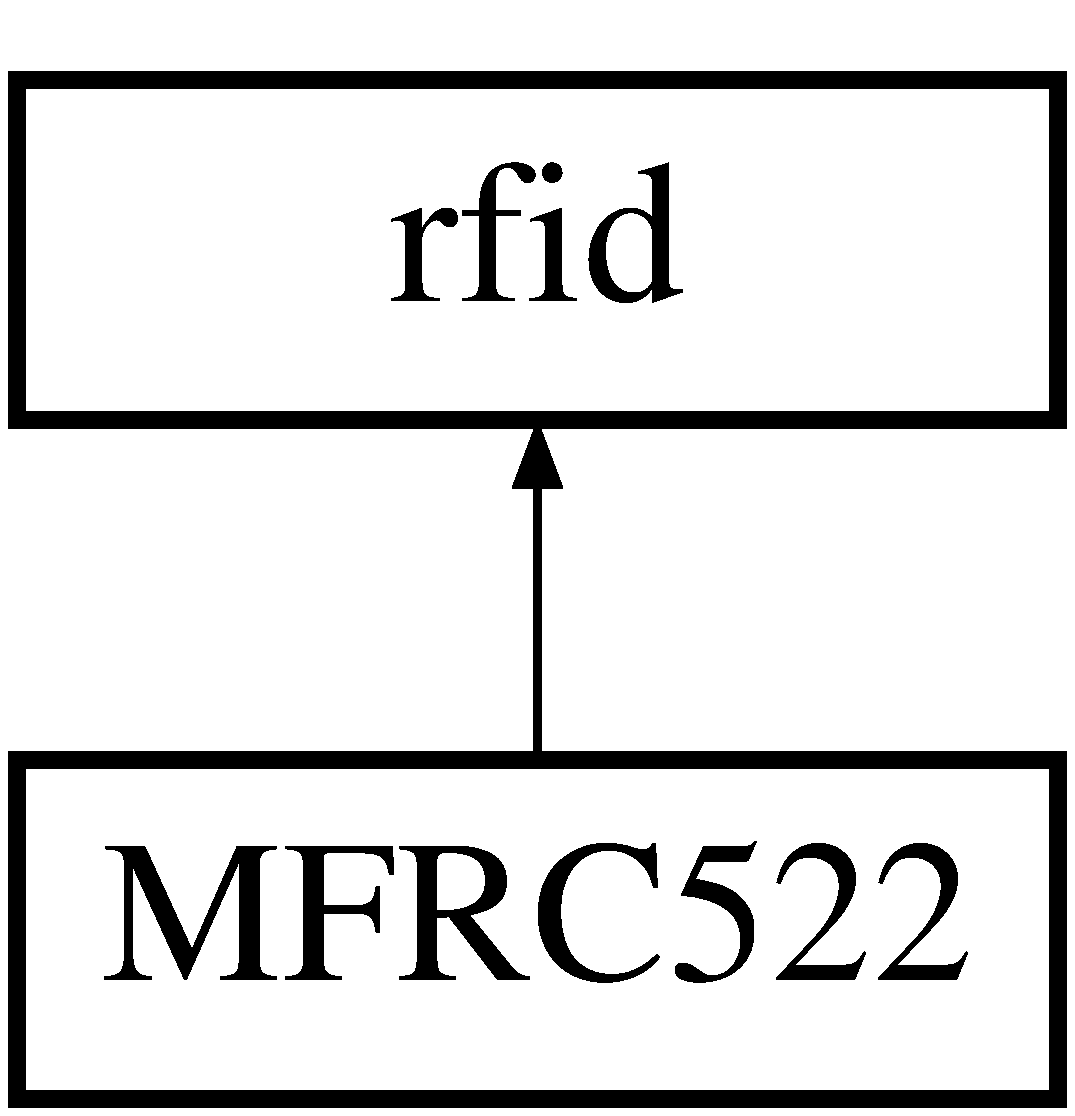
\includegraphics[height=2.000000cm]{classrfid}
\end{center}
\end{figure}
\subsection*{Public Member Functions}
\begin{DoxyCompactItemize}
\item 
virtual void \mbox{\hyperlink{classrfid_a76f857b77fbea6776048aab6ba835a29}{initialize}} ()=0
\begin{DoxyCompactList}\small\item\em Initialize the rfid chip for. \end{DoxyCompactList}\item 
virtual void \mbox{\hyperlink{classrfid_a7f993197e5aa12e7b3bfb1576552bbf1}{hard\+Reset}} ()=0
\begin{DoxyCompactList}\small\item\em Hard reset the rfid chip probably with a hwlib\+::pin\+\_\+out (\href{mailto:wouter@voti.nl}{\tt wouter@voti.\+nl}) 2017. \end{DoxyCompactList}\item 
\mbox{\Hypertarget{classrfid_a880add72f6db49af0b1d23878308d733}\label{classrfid_a880add72f6db49af0b1d23878308d733}} 
virtual void \mbox{\hyperlink{classrfid_a880add72f6db49af0b1d23878308d733}{soft\+Reset}} ()=0
\begin{DoxyCompactList}\small\item\em Soft reset the rfid chip. \end{DoxyCompactList}\item 
virtual void \mbox{\hyperlink{classrfid_abf4826e77ab7b02f04c8f01d969149c1}{reset\+Antennas}} ()=0
\begin{DoxyCompactList}\small\item\em Reset the Tx and Rx antennas. \end{DoxyCompactList}\item 
virtual bool \mbox{\hyperlink{classrfid_a23fc4ec0bc3790c5e68269d4f32771b9}{is\+Card\+In\+Range}} ()=0
\begin{DoxyCompactList}\small\item\em Check if there is a card within the radio frequency field. \end{DoxyCompactList}\item 
virtual bool \mbox{\hyperlink{classrfid_a9790d273f2385c8fb48bb85ca2aa0d10}{is\+Card\+In\+Range\+Check}} ()=0
\begin{DoxyCompactList}\small\item\em Check if there is a card within the radio frequency field. \end{DoxyCompactList}\item 
virtual uint8\+\_\+t \mbox{\hyperlink{classrfid_afeb2a321694ceaf84db793f5efb3a750}{get\+Card\+U\+ID}} (uint8\+\_\+t U\+ID\mbox{[}5\mbox{]})=0
\begin{DoxyCompactList}\small\item\em Get the U\+I\+D/\+N\+U\+ID of 4 bytes U\+ID card with the B\+CC byte. \end{DoxyCompactList}\item 
virtual bool \mbox{\hyperlink{classrfid_aaeb826495120d8d29683f0ea1b985d77}{get\+Card\+U\+I\+D\+Simple}} (uint8\+\_\+t U\+ID\mbox{[}5\mbox{]})=0
\begin{DoxyCompactList}\small\item\em A wrapper around \mbox{\hyperlink{classrfid_afeb2a321694ceaf84db793f5efb3a750}{get\+Card\+U\+ID}} to make it simpler. \end{DoxyCompactList}\item 
virtual void \mbox{\hyperlink{classrfid_a1b324cb1e7b4c377eca4b3495d4189fd}{wait\+For\+Card\+U\+ID}} (uint8\+\_\+t U\+ID\mbox{[}5\mbox{]})=0
\begin{DoxyCompactList}\small\item\em This function waits till there is a card in range and gives the U\+ID back. \end{DoxyCompactList}\item 
virtual void \mbox{\hyperlink{classrfid_a4efe585f73e584d792347c2891300ad2}{print\+U\+ID}} ()=0
\begin{DoxyCompactList}\small\item\em Wait for a card te be presented and print the U\+ID. \end{DoxyCompactList}\item 
virtual bool \mbox{\hyperlink{classrfid_a8c239b8e42f20d4310c44368bd5030a7}{is\+U\+I\+D\+Equal}} (uint8\+\_\+t U\+I\+D1\mbox{[}5\mbox{]}, uint8\+\_\+t U\+I\+D2\mbox{[}5\mbox{]}, unsigned int U\+I\+D\+Size)
\begin{DoxyCompactList}\small\item\em check whether two U\+I\+Ds are equal \end{DoxyCompactList}\item 
virtual bool \mbox{\hyperlink{classrfid_a4ca2918b2b7011a6eb685ea547c21826}{check\+U\+I\+D4\+B\+CC}} (const uint8\+\_\+t U\+ID\mbox{[}5\mbox{]})
\begin{DoxyCompactList}\small\item\em This will check if the U\+ID is valid using B\+CC. \end{DoxyCompactList}\item 
virtual uint8\+\_\+t \mbox{\hyperlink{classrfid_a27619628e718bb781f912aead770079a}{get\+Version}} ()=0
\begin{DoxyCompactList}\small\item\em Get the version of the rfid chip to perform for instance a \mbox{\hyperlink{classrfid_a93e5430380a14fd652e7ca1ce6443198}{self\+Test}}. \end{DoxyCompactList}\item 
virtual bool \mbox{\hyperlink{classrfid_a93e5430380a14fd652e7ca1ce6443198}{self\+Test}} ()=0
\begin{DoxyCompactList}\small\item\em Let the rfid chip perform a self test. \end{DoxyCompactList}\item 
virtual void \mbox{\hyperlink{classrfid_adc4009859b77330fd5b3d0515337ac40}{test}} ()=0
\begin{DoxyCompactList}\small\item\em This checks if the chip is functioning correctly. Make sure you connected everything correctly before executing. \end{DoxyCompactList}\end{DoxyCompactItemize}
\subsection*{Protected Member Functions}
\begin{DoxyCompactItemize}
\item 
\mbox{\Hypertarget{classrfid_aa8c64df0877a6bad52b08cfdcaea02bc}\label{classrfid_aa8c64df0877a6bad52b08cfdcaea02bc}} 
virtual void \mbox{\hyperlink{classrfid_aa8c64df0877a6bad52b08cfdcaea02bc}{wait\+Till\+Started}} ()=0
\begin{DoxyCompactList}\small\item\em Wait till the is started correctly after for example a soft reset. \end{DoxyCompactList}\end{DoxyCompactItemize}


\subsection{Detailed Description}
A pure virtual class for a rfid chip like the \mbox{\hyperlink{class_m_f_r_c522}{M\+F\+R\+C522}}. 

This class is a pure virtual class. This means that you can access methods of the derived class when using reference or pointers. This makes the code easier to expand. \begin{DoxyWarning}{Warning}
T\+HE S\+O\+F\+T\+W\+A\+RE IS P\+R\+O\+V\+I\+D\+ED \char`\"{}\+A\+S I\+S\char`\"{}, W\+I\+T\+H\+O\+UT W\+A\+R\+R\+A\+N\+TY OF A\+NY K\+I\+ND. 
\end{DoxyWarning}


\subsection{Member Function Documentation}
\mbox{\Hypertarget{classrfid_a4ca2918b2b7011a6eb685ea547c21826}\label{classrfid_a4ca2918b2b7011a6eb685ea547c21826}} 
\index{rfid@{rfid}!check\+U\+I\+D4\+B\+CC@{check\+U\+I\+D4\+B\+CC}}
\index{check\+U\+I\+D4\+B\+CC@{check\+U\+I\+D4\+B\+CC}!rfid@{rfid}}
\subsubsection{\texorpdfstring{check\+U\+I\+D4\+B\+C\+C()}{checkUID4BCC()}}
{\footnotesize\ttfamily virtual bool rfid\+::check\+U\+I\+D4\+B\+CC (\begin{DoxyParamCaption}\item[{const uint8\+\_\+t}]{U\+ID\mbox{[}5\mbox{]} }\end{DoxyParamCaption})\hspace{0.3cm}{\ttfamily [inline]}, {\ttfamily [virtual]}}



This will check if the U\+ID is valid using B\+CC. 


\begin{DoxyParams}{Parameters}
{\em U\+I\+D\mbox{[}$\,$\mbox{]}} & the array where the U\+ID including the B\+CC is store.\\
\hline
\end{DoxyParams}
The U\+ID\mbox{[}5\mbox{]} will N\+OT be changed using this function. This check was found on the following site\+: \href{http://www.proxmark.org/forum/viewtopic.php?id=2274}{\tt B\+CC check} \mbox{\Hypertarget{classrfid_afeb2a321694ceaf84db793f5efb3a750}\label{classrfid_afeb2a321694ceaf84db793f5efb3a750}} 
\index{rfid@{rfid}!get\+Card\+U\+ID@{get\+Card\+U\+ID}}
\index{get\+Card\+U\+ID@{get\+Card\+U\+ID}!rfid@{rfid}}
\subsubsection{\texorpdfstring{get\+Card\+U\+I\+D()}{getCardUID()}}
{\footnotesize\ttfamily virtual uint8\+\_\+t rfid\+::get\+Card\+U\+ID (\begin{DoxyParamCaption}\item[{uint8\+\_\+t}]{U\+ID\mbox{[}5\mbox{]} }\end{DoxyParamCaption})\hspace{0.3cm}{\ttfamily [pure virtual]}}



Get the U\+I\+D/\+N\+U\+ID of 4 bytes U\+ID card with the B\+CC byte. 


\begin{DoxyParams}{Parameters}
{\em U\+I\+D\mbox{[}$\,$\mbox{]}} & The array you want the U\+ID to get stored into. \\
\hline
\end{DoxyParams}
\begin{DoxyReturn}{Returns}
An uint8\+\_\+t containing a possible error or succes code. (These codes are in the derived class)
\end{DoxyReturn}
The U\+ID of a card is a unique identifier. This U\+ID can be used to know which card you\textquotesingle{}re communicating with. The U\+ID is used when more than one card is in the radio frequency field, also known as collision detection.~\newline
 The last byte of U\+ID\mbox{[}5\mbox{]} will be the bcc. This can be used to check if the U\+ID is valid. \begin{DoxyWarning}{Warning}
Note that the U\+ID might not be as unique as you might expect. Some cards have a feature to rewrite the U\+ID block. 

Note that the U\+ID\mbox{[}5\mbox{]} array will be overridden. 
\end{DoxyWarning}


Implemented in \mbox{\hyperlink{class_m_f_r_c522_ad3c7ab4c70988e80c400f36f724a12b7}{M\+F\+R\+C522}}.

\mbox{\Hypertarget{classrfid_aaeb826495120d8d29683f0ea1b985d77}\label{classrfid_aaeb826495120d8d29683f0ea1b985d77}} 
\index{rfid@{rfid}!get\+Card\+U\+I\+D\+Simple@{get\+Card\+U\+I\+D\+Simple}}
\index{get\+Card\+U\+I\+D\+Simple@{get\+Card\+U\+I\+D\+Simple}!rfid@{rfid}}
\subsubsection{\texorpdfstring{get\+Card\+U\+I\+D\+Simple()}{getCardUIDSimple()}}
{\footnotesize\ttfamily virtual bool rfid\+::get\+Card\+U\+I\+D\+Simple (\begin{DoxyParamCaption}\item[{uint8\+\_\+t}]{U\+ID\mbox{[}5\mbox{]} }\end{DoxyParamCaption})\hspace{0.3cm}{\ttfamily [pure virtual]}}



A wrapper around \mbox{\hyperlink{classrfid_afeb2a321694ceaf84db793f5efb3a750}{get\+Card\+U\+ID}} to make it simpler. 


\begin{DoxyParams}{Parameters}
{\em U\+I\+D\mbox{[}$\,$\mbox{]}} & The array you want the U\+ID to get stored into. \\
\hline
\end{DoxyParams}
\begin{DoxyReturn}{Returns}
A bool which will be 1 when everything went fine and 0 when there was an error.
\end{DoxyReturn}
When the function returns a zero you should try \mbox{\hyperlink{classrfid_afeb2a321694ceaf84db793f5efb3a750}{get\+Card\+U\+ID}} instead because that function returns a more accurate return status. \begin{DoxyWarning}{Warning}
Note that the U\+ID might not be as unique as you might expect. Some cards have a feature to rewrite the U\+ID block. 

Note that the U\+ID\mbox{[}5\mbox{]} array will be overridden. 
\end{DoxyWarning}


Implemented in \mbox{\hyperlink{class_m_f_r_c522_a33c20be6030f635d986984db4999a1eb}{M\+F\+R\+C522}}.

\mbox{\Hypertarget{classrfid_a27619628e718bb781f912aead770079a}\label{classrfid_a27619628e718bb781f912aead770079a}} 
\index{rfid@{rfid}!get\+Version@{get\+Version}}
\index{get\+Version@{get\+Version}!rfid@{rfid}}
\subsubsection{\texorpdfstring{get\+Version()}{getVersion()}}
{\footnotesize\ttfamily virtual uint8\+\_\+t rfid\+::get\+Version (\begin{DoxyParamCaption}{ }\end{DoxyParamCaption})\hspace{0.3cm}{\ttfamily [pure virtual]}}



Get the version of the rfid chip to perform for instance a \mbox{\hyperlink{classrfid_a93e5430380a14fd652e7ca1ce6443198}{self\+Test}}. 

\begin{DoxyReturn}{Returns}
An uint8\+\_\+t containing the version value 1 or 2 
\end{DoxyReturn}


Implemented in \mbox{\hyperlink{class_m_f_r_c522_a25fb0a50bf7db51ab9c5bc2ff4fa84e3}{M\+F\+R\+C522}}.

\mbox{\Hypertarget{classrfid_a7f993197e5aa12e7b3bfb1576552bbf1}\label{classrfid_a7f993197e5aa12e7b3bfb1576552bbf1}} 
\index{rfid@{rfid}!hard\+Reset@{hard\+Reset}}
\index{hard\+Reset@{hard\+Reset}!rfid@{rfid}}
\subsubsection{\texorpdfstring{hard\+Reset()}{hardReset()}}
{\footnotesize\ttfamily virtual void rfid\+::hard\+Reset (\begin{DoxyParamCaption}{ }\end{DoxyParamCaption})\hspace{0.3cm}{\ttfamily [pure virtual]}}



Hard reset the rfid chip probably with a hwlib\+::pin\+\_\+out (\href{mailto:wouter@voti.nl}{\tt wouter@voti.\+nl}) 2017. 

\begin{DoxyWarning}{Warning}
Note if the chip requires a external pin to reset the whole chip. The pin must me connected correctly. 
\end{DoxyWarning}


Implemented in \mbox{\hyperlink{class_m_f_r_c522_a016df9ed0421397c634cc79c475dbe3b}{M\+F\+R\+C522}}.

\mbox{\Hypertarget{classrfid_a76f857b77fbea6776048aab6ba835a29}\label{classrfid_a76f857b77fbea6776048aab6ba835a29}} 
\index{rfid@{rfid}!initialize@{initialize}}
\index{initialize@{initialize}!rfid@{rfid}}
\subsubsection{\texorpdfstring{initialize()}{initialize()}}
{\footnotesize\ttfamily virtual void rfid\+::initialize (\begin{DoxyParamCaption}{ }\end{DoxyParamCaption})\hspace{0.3cm}{\ttfamily [pure virtual]}}



Initialize the rfid chip for. 

This will reset the chip and initilize all the register. 

Implemented in \mbox{\hyperlink{class_m_f_r_c522_a5f589b09eaf150551b369052ce125fa1}{M\+F\+R\+C522}}.

\mbox{\Hypertarget{classrfid_a23fc4ec0bc3790c5e68269d4f32771b9}\label{classrfid_a23fc4ec0bc3790c5e68269d4f32771b9}} 
\index{rfid@{rfid}!is\+Card\+In\+Range@{is\+Card\+In\+Range}}
\index{is\+Card\+In\+Range@{is\+Card\+In\+Range}!rfid@{rfid}}
\subsubsection{\texorpdfstring{is\+Card\+In\+Range()}{isCardInRange()}}
{\footnotesize\ttfamily virtual bool rfid\+::is\+Card\+In\+Range (\begin{DoxyParamCaption}{ }\end{DoxyParamCaption})\hspace{0.3cm}{\ttfamily [pure virtual]}}



Check if there is a card within the radio frequency field. 

\begin{DoxyReturn}{Returns}
A bool which will be 1 if a card is detected and 0 when not.
\end{DoxyReturn}
This function checks whether there is a card within the radio frequency field. The function uses the rfid request command to achieve this. \begin{DoxyWarning}{Warning}
After requesting the rfid card expects the user to send another command. When you you only want to check if a card is in the radio frequency field you should use is\+Card\+In\+Range\+Check 
\end{DoxyWarning}


Implemented in \mbox{\hyperlink{class_m_f_r_c522_a019f76569bddf9c2f9f94eca13a618d7}{M\+F\+R\+C522}}.

\mbox{\Hypertarget{classrfid_a9790d273f2385c8fb48bb85ca2aa0d10}\label{classrfid_a9790d273f2385c8fb48bb85ca2aa0d10}} 
\index{rfid@{rfid}!is\+Card\+In\+Range\+Check@{is\+Card\+In\+Range\+Check}}
\index{is\+Card\+In\+Range\+Check@{is\+Card\+In\+Range\+Check}!rfid@{rfid}}
\subsubsection{\texorpdfstring{is\+Card\+In\+Range\+Check()}{isCardInRangeCheck()}}
{\footnotesize\ttfamily virtual bool rfid\+::is\+Card\+In\+Range\+Check (\begin{DoxyParamCaption}{ }\end{DoxyParamCaption})\hspace{0.3cm}{\ttfamily [pure virtual]}}



Check if there is a card within the radio frequency field. 

\begin{DoxyReturn}{Returns}
A bool which will be 1 if a card is detected and 0 when not.
\end{DoxyReturn}
This function checks whether there is a card within the radio frequency field. The function uses the rfid request command to achieve this. After sending the request command both antennas are reset (\mbox{\hyperlink{classrfid_abf4826e77ab7b02f04c8f01d969149c1}{reset\+Antennas}}) to stop communicating with the card. \begin{DoxyWarning}{Warning}
Use \mbox{\hyperlink{classrfid_a23fc4ec0bc3790c5e68269d4f32771b9}{is\+Card\+In\+Range}} when you want to send some commands after you send a request to the card. 
\end{DoxyWarning}


Implemented in \mbox{\hyperlink{class_m_f_r_c522_a29ce0dd04495f9352e32ada5ecc5fd03}{M\+F\+R\+C522}}.

\mbox{\Hypertarget{classrfid_a8c239b8e42f20d4310c44368bd5030a7}\label{classrfid_a8c239b8e42f20d4310c44368bd5030a7}} 
\index{rfid@{rfid}!is\+U\+I\+D\+Equal@{is\+U\+I\+D\+Equal}}
\index{is\+U\+I\+D\+Equal@{is\+U\+I\+D\+Equal}!rfid@{rfid}}
\subsubsection{\texorpdfstring{is\+U\+I\+D\+Equal()}{isUIDEqual()}}
{\footnotesize\ttfamily virtual bool rfid\+::is\+U\+I\+D\+Equal (\begin{DoxyParamCaption}\item[{uint8\+\_\+t}]{U\+I\+D1\mbox{[}5\mbox{]},  }\item[{uint8\+\_\+t}]{U\+I\+D2\mbox{[}5\mbox{]},  }\item[{unsigned int}]{U\+I\+D\+Size }\end{DoxyParamCaption})\hspace{0.3cm}{\ttfamily [inline]}, {\ttfamily [virtual]}}



check whether two U\+I\+Ds are equal 


\begin{DoxyParams}{Parameters}
{\em U\+I\+D1\mbox{[}$\,$\mbox{]}} & the first U\+ID you want to check. \\
\hline
{\em U\+I\+D2\mbox{[}$\,$\mbox{]}} & the seconds U\+ID you want to check. \\
\hline
{\em U\+I\+D\+Size} & the size of the arrays. N\+O\+TE T\+H\+AT F\+OR N\+OW T\+H\+EY H\+A\+VE TO BE 5. \\
\hline
\end{DoxyParams}
\begin{DoxyReturn}{Returns}
A bool containing a 1 when they\textquotesingle{}re the same and a zero when the\textquotesingle{}re not.
\end{DoxyReturn}
This method will check if every value of the same index in the arrays are equal. The B\+CC is also checked for equality. \mbox{\Hypertarget{classrfid_a4efe585f73e584d792347c2891300ad2}\label{classrfid_a4efe585f73e584d792347c2891300ad2}} 
\index{rfid@{rfid}!print\+U\+ID@{print\+U\+ID}}
\index{print\+U\+ID@{print\+U\+ID}!rfid@{rfid}}
\subsubsection{\texorpdfstring{print\+U\+I\+D()}{printUID()}}
{\footnotesize\ttfamily virtual void rfid\+::print\+U\+ID (\begin{DoxyParamCaption}{ }\end{DoxyParamCaption})\hspace{0.3cm}{\ttfamily [pure virtual]}}



Wait for a card te be presented and print the U\+ID. 

This method waits for a card to be presented. After a card has been detected the U\+ID will be printed to the terminal. \begin{DoxyWarning}{Warning}
This function blocks everything! 
\end{DoxyWarning}


Implemented in \mbox{\hyperlink{class_m_f_r_c522_aee85264d7411b76a3b0817622b428827}{M\+F\+R\+C522}}.

\mbox{\Hypertarget{classrfid_abf4826e77ab7b02f04c8f01d969149c1}\label{classrfid_abf4826e77ab7b02f04c8f01d969149c1}} 
\index{rfid@{rfid}!reset\+Antennas@{reset\+Antennas}}
\index{reset\+Antennas@{reset\+Antennas}!rfid@{rfid}}
\subsubsection{\texorpdfstring{reset\+Antennas()}{resetAntennas()}}
{\footnotesize\ttfamily virtual void rfid\+::reset\+Antennas (\begin{DoxyParamCaption}{ }\end{DoxyParamCaption})\hspace{0.3cm}{\ttfamily [pure virtual]}}



Reset the Tx and Rx antennas. 

This function is mostly used to stop communicating with a card without using the halt command. 

Implemented in \mbox{\hyperlink{class_m_f_r_c522_ac981022cc3ae79f727b2365e309cf691}{M\+F\+R\+C522}}.

\mbox{\Hypertarget{classrfid_a93e5430380a14fd652e7ca1ce6443198}\label{classrfid_a93e5430380a14fd652e7ca1ce6443198}} 
\index{rfid@{rfid}!self\+Test@{self\+Test}}
\index{self\+Test@{self\+Test}!rfid@{rfid}}
\subsubsection{\texorpdfstring{self\+Test()}{selfTest()}}
{\footnotesize\ttfamily virtual bool rfid\+::self\+Test (\begin{DoxyParamCaption}{ }\end{DoxyParamCaption})\hspace{0.3cm}{\ttfamily [pure virtual]}}



Let the rfid chip perform a self test. 

\begin{DoxyReturn}{Returns}
A bool containing a 1 when passed and 0 when failed the self test.
\end{DoxyReturn}
The rfid chip performs a self test. The self testing sequence can be found in the datasheet \href{https://www.nxp.com/docs/en/data-sheet/MFRC522.pdf}{\tt M\+F\+R\+C522 datasheet page 85} \begin{DoxyWarning}{Warning}
Only version 1 and 2 are supported at the moment! Some clones might have another version. It might work fine when not passing the test. 
\end{DoxyWarning}


Implemented in \mbox{\hyperlink{class_m_f_r_c522_adcc4f5eb212c1a94e462eab459bd685e}{M\+F\+R\+C522}}.

\mbox{\Hypertarget{classrfid_adc4009859b77330fd5b3d0515337ac40}\label{classrfid_adc4009859b77330fd5b3d0515337ac40}} 
\index{rfid@{rfid}!test@{test}}
\index{test@{test}!rfid@{rfid}}
\subsubsection{\texorpdfstring{test()}{test()}}
{\footnotesize\ttfamily virtual void rfid\+::test (\begin{DoxyParamCaption}{ }\end{DoxyParamCaption})\hspace{0.3cm}{\ttfamily [pure virtual]}}



This checks if the chip is functioning correctly. Make sure you connected everything correctly before executing. 

Testing might take a while. Wait till the end test message appears. Testing requires a rfid 4 U\+ID sized card. 

Implemented in \mbox{\hyperlink{class_m_f_r_c522_aff8e84921e9f133cfbd243ce994da023}{M\+F\+R\+C522}}.

\mbox{\Hypertarget{classrfid_a1b324cb1e7b4c377eca4b3495d4189fd}\label{classrfid_a1b324cb1e7b4c377eca4b3495d4189fd}} 
\index{rfid@{rfid}!wait\+For\+Card\+U\+ID@{wait\+For\+Card\+U\+ID}}
\index{wait\+For\+Card\+U\+ID@{wait\+For\+Card\+U\+ID}!rfid@{rfid}}
\subsubsection{\texorpdfstring{wait\+For\+Card\+U\+I\+D()}{waitForCardUID()}}
{\footnotesize\ttfamily virtual void rfid\+::wait\+For\+Card\+U\+ID (\begin{DoxyParamCaption}\item[{uint8\+\_\+t}]{U\+ID\mbox{[}5\mbox{]} }\end{DoxyParamCaption})\hspace{0.3cm}{\ttfamily [pure virtual]}}



This function waits till there is a card in range and gives the U\+ID back. 

\begin{DoxyWarning}{Warning}
This function blocks everything! And will continue when there is a card detected with valid U\+ID. 
\end{DoxyWarning}


Implemented in \mbox{\hyperlink{class_m_f_r_c522_aeb05c83c2d139eb2c57f400399982691}{M\+F\+R\+C522}}.



The documentation for this class was generated from the following file\+:\begin{DoxyCompactItemize}
\item 
Demo/rfid.\+hpp\end{DoxyCompactItemize}

\hypertarget{classspi_bus}{}\section{spi\+Bus Class Reference}
\label{classspi_bus}\index{spi\+Bus@{spi\+Bus}}


Basic S\+PI functions like write and read a register.  




{\ttfamily \#include $<$spi\+Bus.\+hpp$>$}

Inheritance diagram for spi\+Bus\+:\begin{figure}[H]
\begin{center}
\leavevmode
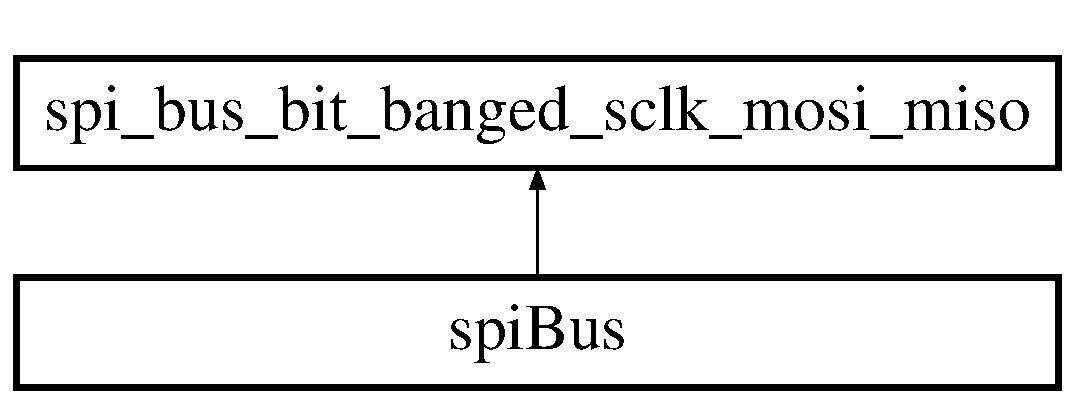
\includegraphics[height=2.000000cm]{classspi_bus}
\end{center}
\end{figure}
\subsection*{Public Member Functions}
\begin{DoxyCompactItemize}
\item 
\mbox{\hyperlink{classspi_bus_a042e32891d6fffd4b4eb706600244062}{spi\+Bus}} (hwlib\+::pin\+\_\+out \&scl, hwlib\+::pin\+\_\+out \&mosi, hwlib\+::pin\+\_\+in \&miso)
\begin{DoxyCompactList}\small\item\em This is a constructor for the Spi\+Bus class. \end{DoxyCompactList}\item 
uint8\+\_\+t \mbox{\hyperlink{classspi_bus_ab6b195b235dd0a1dad2f7cec3d997ffb}{get\+Byte\+From\+Register}} (const uint8\+\_\+t chip\+Reg\+Address, hwlib\+::pin\+\_\+out \&slave\+Select)
\begin{DoxyCompactList}\small\item\em Get only one byte from a specific register. \end{DoxyCompactList}\item 
void \mbox{\hyperlink{classspi_bus_a58318fdc7b4ff1869be4f0f321a853a8}{get\+Bytes\+From\+Register}} (const uint8\+\_\+t chip\+Reg\+Address, uint8\+\_\+t data\mbox{[}$\,$\mbox{]}, const uint8\+\_\+t amount\+Of\+Bytes, hwlib\+::pin\+\_\+out \&slave\+Select)
\begin{DoxyCompactList}\small\item\em Get multiple byte from a specific register. \end{DoxyCompactList}\item 
void \mbox{\hyperlink{classspi_bus_a3322a039f33a7180a9a57da662607b7d}{set\+Byte\+In\+Register}} (const uint8\+\_\+t chip\+Reg\+Address, uint8\+\_\+t byte, hwlib\+::pin\+\_\+out \&slave\+Select)
\begin{DoxyCompactList}\small\item\em Set a byte into a specific register. \end{DoxyCompactList}\item 
void \mbox{\hyperlink{classspi_bus_a734591a2184ce01cac6dcf875ac424d4}{set\+Bytes\+In\+Register}} (const uint8\+\_\+t chip\+Reg\+Address, uint8\+\_\+t new\+Bytes\mbox{[}$\,$\mbox{]}, const uint8\+\_\+t amount\+Of\+Bytes, hwlib\+::pin\+\_\+out \&slave\+Select)
\begin{DoxyCompactList}\small\item\em Set multiple bytes starting from a specific register. \end{DoxyCompactList}\end{DoxyCompactItemize}
\subsection*{Private Member Functions}
\begin{DoxyCompactItemize}
\item 
uint8\+\_\+t \mbox{\hyperlink{classspi_bus_a6e5f0193b056b4b58db49e1c6ce5d807}{get\+Read\+Byte}} (const uint8\+\_\+t chip\+Reg\+Address)
\begin{DoxyCompactList}\small\item\em this function will create a read byte using a specific register. \end{DoxyCompactList}\item 
uint8\+\_\+t \mbox{\hyperlink{classspi_bus_af09ae8625cbb1c5353e3777af6bf5ae3}{get\+Write\+Byte}} (const uint8\+\_\+t chip\+Reg\+Address)
\begin{DoxyCompactList}\small\item\em this function will create a write byte using a specific register. \end{DoxyCompactList}\end{DoxyCompactItemize}
\subsection*{Private Attributes}
\begin{DoxyCompactItemize}
\item 
const uint8\+\_\+t \mbox{\hyperlink{classspi_bus_a0dda31f7fa031ef8913e029d2eb4acf9}{R\+E\+A\+D\+\_\+\+M\+A\+SK}} = 0x80
\begin{DoxyCompactList}\small\item\em This mask should be used before sending the register byte W\+H\+EN R\+E\+A\+D\+I\+NG. \end{DoxyCompactList}\item 
const uint8\+\_\+t \mbox{\hyperlink{classspi_bus_acd898d08216428963563e20f033423b3}{R\+E\+G\+I\+S\+T\+E\+R\+\_\+\+M\+A\+SK}} = 0x7E
\begin{DoxyCompactList}\small\item\em This mask should be used before sending the register byte when reading or writing. \end{DoxyCompactList}\end{DoxyCompactItemize}


\subsection{Detailed Description}
Basic S\+PI functions like write and read a register. 

This class is a wrapper around the hwlib\+::spi\+\_\+bus\+\_\+bit\+\_\+banged\+\_\+sclk\+\_\+mosi\+\_\+miso (\href{mailto:wouter@voti.nl}{\tt wouter@voti.\+nl} 2017). It contains some basic S\+PI functions for easy access of the used chip. \begin{DoxyWarning}{Warning}
T\+HE S\+O\+F\+T\+W\+A\+RE IS P\+R\+O\+V\+I\+D\+ED \char`\"{}\+A\+S I\+S\char`\"{}, W\+I\+T\+H\+O\+UT W\+A\+R\+R\+A\+N\+TY OF A\+NY K\+I\+ND. 
\end{DoxyWarning}


\subsection{Constructor \& Destructor Documentation}
\mbox{\Hypertarget{classspi_bus_a042e32891d6fffd4b4eb706600244062}\label{classspi_bus_a042e32891d6fffd4b4eb706600244062}} 
\index{spi\+Bus@{spi\+Bus}!spi\+Bus@{spi\+Bus}}
\index{spi\+Bus@{spi\+Bus}!spi\+Bus@{spi\+Bus}}
\subsubsection{\texorpdfstring{spi\+Bus()}{spiBus()}}
{\footnotesize\ttfamily spi\+Bus\+::spi\+Bus (\begin{DoxyParamCaption}\item[{hwlib\+::pin\+\_\+out \&}]{scl,  }\item[{hwlib\+::pin\+\_\+out \&}]{mosi,  }\item[{hwlib\+::pin\+\_\+in \&}]{miso }\end{DoxyParamCaption})}



This is a constructor for the Spi\+Bus class. 


\begin{DoxyParams}{Parameters}
{\em scl} & the Serial Clock Line. \\
\hline
{\em mosi} & the Master Output Slave Input, data from master -\/$>$ slave. \\
\hline
{\em miso} & the Master Input Slave Output, data from slave -\/$>$ master. \\
\hline
\end{DoxyParams}


\subsection{Member Function Documentation}
\mbox{\Hypertarget{classspi_bus_ab6b195b235dd0a1dad2f7cec3d997ffb}\label{classspi_bus_ab6b195b235dd0a1dad2f7cec3d997ffb}} 
\index{spi\+Bus@{spi\+Bus}!get\+Byte\+From\+Register@{get\+Byte\+From\+Register}}
\index{get\+Byte\+From\+Register@{get\+Byte\+From\+Register}!spi\+Bus@{spi\+Bus}}
\subsubsection{\texorpdfstring{get\+Byte\+From\+Register()}{getByteFromRegister()}}
{\footnotesize\ttfamily uint8\+\_\+t spi\+Bus\+::get\+Byte\+From\+Register (\begin{DoxyParamCaption}\item[{const uint8\+\_\+t}]{chip\+Reg\+Address,  }\item[{hwlib\+::pin\+\_\+out \&}]{slave\+Select }\end{DoxyParamCaption})}



Get only one byte from a specific register. 


\begin{DoxyParams}{Parameters}
{\em chip\+Reg\+Address} & the register you want to get the byte of. \\
\hline
{\em slave\+Select} & the pin the slave select of the slave you want to read from. \\
\hline
\end{DoxyParams}
\begin{DoxyReturn}{Returns}
A uint8\+\_\+t which contains the byte of the given register.
\end{DoxyReturn}
This method sends one bytes to the slave over the mosi. The first byte is the read register byte created by \mbox{\hyperlink{classspi_bus_a6e5f0193b056b4b58db49e1c6ce5d807}{get\+Read\+Byte}}. After sending the byte the miso will receive the byte of the chip\+Reg\+Address. The data is send and received by hwlib\+::spi\+\_\+bus\+\_\+bit\+\_\+banged\+\_\+sclk\+\_\+mosi\+\_\+miso.\+write\+\_\+and\+\_\+read() (\href{mailto:wouter@voti.nl}{\tt wouter@voti.\+nl} 2017) \mbox{\Hypertarget{classspi_bus_a58318fdc7b4ff1869be4f0f321a853a8}\label{classspi_bus_a58318fdc7b4ff1869be4f0f321a853a8}} 
\index{spi\+Bus@{spi\+Bus}!get\+Bytes\+From\+Register@{get\+Bytes\+From\+Register}}
\index{get\+Bytes\+From\+Register@{get\+Bytes\+From\+Register}!spi\+Bus@{spi\+Bus}}
\subsubsection{\texorpdfstring{get\+Bytes\+From\+Register()}{getBytesFromRegister()}}
{\footnotesize\ttfamily void spi\+Bus\+::get\+Bytes\+From\+Register (\begin{DoxyParamCaption}\item[{const uint8\+\_\+t}]{chip\+Reg\+Address,  }\item[{uint8\+\_\+t}]{data\mbox{[}$\,$\mbox{]},  }\item[{const uint8\+\_\+t}]{amount\+Of\+Bytes,  }\item[{hwlib\+::pin\+\_\+out \&}]{slave\+Select }\end{DoxyParamCaption})}



Get multiple byte from a specific register. 


\begin{DoxyParams}{Parameters}
{\em chip\+Reg\+Address} & the register you want the bytes from. \\
\hline
{\em data\mbox{[}$\,$\mbox{]}} & a pointer to an array where the bytes will be stored in. \\
\hline
{\em amount\+Of\+Bytes} & the amount of bytes you want to get. \\
\hline
{\em slave\+Select} & the pin the slave select of the slave you want to read from.\\
\hline
\end{DoxyParams}
First this function creates a new array to store the retreived data in. This array will be one step bigger than the amount\+Of\+Bytes you want to retreive. After creating the array a read byte using the chip\+Reg\+Address and \mbox{\hyperlink{classspi_bus_a6e5f0193b056b4b58db49e1c6ce5d807}{get\+Read\+Byte}} The array will be filled with this read byte. After using hwlib\+::spi\+\_\+bus\+\_\+bit\+\_\+banged\+\_\+sclk\+\_\+mosi\+\_\+miso.\+write\+\_\+and\+\_\+read() (\href{mailto:wouter@voti.nl}{\tt wouter@voti.\+nl} 2017) It will fill your given array with the retreived data. \begin{DoxyWarning}{Warning}
The size of the array must at least be the amount\+Of\+Bytes! 

The given chip\+Reg\+Address will read multiple times. Some registers will be empty after reading. R\+E\+AD T\+HE D\+A\+T\+A\+S\+H\+E\+ET B\+E\+F\+O\+RE U\+S\+I\+N\+G! 
\end{DoxyWarning}
\mbox{\Hypertarget{classspi_bus_a6e5f0193b056b4b58db49e1c6ce5d807}\label{classspi_bus_a6e5f0193b056b4b58db49e1c6ce5d807}} 
\index{spi\+Bus@{spi\+Bus}!get\+Read\+Byte@{get\+Read\+Byte}}
\index{get\+Read\+Byte@{get\+Read\+Byte}!spi\+Bus@{spi\+Bus}}
\subsubsection{\texorpdfstring{get\+Read\+Byte()}{getReadByte()}}
{\footnotesize\ttfamily uint8\+\_\+t spi\+Bus\+::get\+Read\+Byte (\begin{DoxyParamCaption}\item[{const uint8\+\_\+t}]{chip\+Reg\+Address }\end{DoxyParamCaption})\hspace{0.3cm}{\ttfamily [private]}}



this function will create a read byte using a specific register. 


\begin{DoxyParams}{Parameters}
{\em chip\+Reg\+Address} & the register address you want to get the read chip register byte of. \\
\hline
\end{DoxyParams}
\begin{DoxyReturn}{Returns}
A uint8\+\_\+t which contains the read register byte.
\end{DoxyReturn}
The read register byte is the chip\+Reg\+Address shifted one bit to the left and the \mbox{\hyperlink{classspi_bus_acd898d08216428963563e20f033423b3}{R\+E\+G\+I\+S\+T\+E\+R\+\_\+\+M\+A\+SK}} and \mbox{\hyperlink{classspi_bus_a0dda31f7fa031ef8913e029d2eb4acf9}{R\+E\+A\+D\+\_\+\+M\+A\+SK}} operated on it. \mbox{\Hypertarget{classspi_bus_af09ae8625cbb1c5353e3777af6bf5ae3}\label{classspi_bus_af09ae8625cbb1c5353e3777af6bf5ae3}} 
\index{spi\+Bus@{spi\+Bus}!get\+Write\+Byte@{get\+Write\+Byte}}
\index{get\+Write\+Byte@{get\+Write\+Byte}!spi\+Bus@{spi\+Bus}}
\subsubsection{\texorpdfstring{get\+Write\+Byte()}{getWriteByte()}}
{\footnotesize\ttfamily uint8\+\_\+t spi\+Bus\+::get\+Write\+Byte (\begin{DoxyParamCaption}\item[{const uint8\+\_\+t}]{chip\+Reg\+Address }\end{DoxyParamCaption})\hspace{0.3cm}{\ttfamily [private]}}



this function will create a write byte using a specific register. 


\begin{DoxyParams}{Parameters}
{\em chip\+Reg\+Address} & the register address you want to get the write chip register byte of. \\
\hline
\end{DoxyParams}
\begin{DoxyReturn}{Returns}
A uint8\+\_\+t which contains the write register byte.
\end{DoxyReturn}
The write register byte is the chip\+Reg\+Address shifted one bit to the left and the \mbox{\hyperlink{classspi_bus_acd898d08216428963563e20f033423b3}{R\+E\+G\+I\+S\+T\+E\+R\+\_\+\+M\+A\+SK}} operated on it. \mbox{\Hypertarget{classspi_bus_a3322a039f33a7180a9a57da662607b7d}\label{classspi_bus_a3322a039f33a7180a9a57da662607b7d}} 
\index{spi\+Bus@{spi\+Bus}!set\+Byte\+In\+Register@{set\+Byte\+In\+Register}}
\index{set\+Byte\+In\+Register@{set\+Byte\+In\+Register}!spi\+Bus@{spi\+Bus}}
\subsubsection{\texorpdfstring{set\+Byte\+In\+Register()}{setByteInRegister()}}
{\footnotesize\ttfamily void spi\+Bus\+::set\+Byte\+In\+Register (\begin{DoxyParamCaption}\item[{const uint8\+\_\+t}]{chip\+Reg\+Address,  }\item[{uint8\+\_\+t}]{byte,  }\item[{hwlib\+::pin\+\_\+out \&}]{slave\+Select }\end{DoxyParamCaption})}



Set a byte into a specific register. 


\begin{DoxyParams}{Parameters}
{\em chip\+Reg\+Address} & the register you want the byte of. \\
\hline
{\em byte} & the byte you want to set into the chip\+Reg\+Address. \\
\hline
{\em slave\+Select} & the pin the slave select of the slave you want to write to.\\
\hline
\end{DoxyParams}
A array will be created and a write register byte will be set to the first index. The write register byte will be generated using \mbox{\hyperlink{classspi_bus_af09ae8625cbb1c5353e3777af6bf5ae3}{get\+Write\+Byte}}. The second index of the array will be the byte you want to sent. The bytes will be send using hwlib\+::spi\+\_\+bus\+\_\+bit\+\_\+banged\+\_\+sclk\+\_\+mosi\+\_\+miso.\+write\+\_\+and\+\_\+read() (\href{mailto:wouter@voti.nl}{\tt wouter@voti.\+nl} 2017) \begin{DoxyWarning}{Warning}
The value in the register will be overridden. 
\end{DoxyWarning}
\mbox{\Hypertarget{classspi_bus_a734591a2184ce01cac6dcf875ac424d4}\label{classspi_bus_a734591a2184ce01cac6dcf875ac424d4}} 
\index{spi\+Bus@{spi\+Bus}!set\+Bytes\+In\+Register@{set\+Bytes\+In\+Register}}
\index{set\+Bytes\+In\+Register@{set\+Bytes\+In\+Register}!spi\+Bus@{spi\+Bus}}
\subsubsection{\texorpdfstring{set\+Bytes\+In\+Register()}{setBytesInRegister()}}
{\footnotesize\ttfamily void spi\+Bus\+::set\+Bytes\+In\+Register (\begin{DoxyParamCaption}\item[{const uint8\+\_\+t}]{chip\+Reg\+Address,  }\item[{uint8\+\_\+t}]{new\+Bytes\mbox{[}$\,$\mbox{]},  }\item[{const uint8\+\_\+t}]{amount\+Of\+Bytes,  }\item[{hwlib\+::pin\+\_\+out \&}]{slave\+Select }\end{DoxyParamCaption})}



Set multiple bytes starting from a specific register. 


\begin{DoxyParams}{Parameters}
{\em chip\+Reg\+Address} & the register you want start getting the bytes from. \\
\hline
{\em new\+Bytes\mbox{[}$\,$\mbox{]}} & a pointer to an array where the bytes you want to send are stored. \\
\hline
{\em amount\+Of\+Bytes} & the amount of bytes you want to set. \\
\hline
{\em slave\+Select} & the pin the slave select of the slave you want to write to.\\
\hline
\end{DoxyParams}
First a new array will be created one size bigger than amount\+Of\+Bytes. The first byte will be the register write byte generated by \mbox{\hyperlink{classspi_bus_af09ae8625cbb1c5353e3777af6bf5ae3}{get\+Write\+Byte}}. The rest of the array will be filled with the data in the new\+Bytes array. After setting up the array it will be send to the chip using hwlib\+::spi\+\_\+bus\+\_\+bit\+\_\+banged\+\_\+sclk\+\_\+mosi\+\_\+miso.\+write\+\_\+and\+\_\+read() (\href{mailto:wouter@voti.nl}{\tt wouter@voti.\+nl} 2017). \begin{DoxyWarning}{Warning}
The size of new\+Bytes\mbox{[}\mbox{]} should be amount\+Of\+Bytes. 
\end{DoxyWarning}


\subsection{Member Data Documentation}
\mbox{\Hypertarget{classspi_bus_a0dda31f7fa031ef8913e029d2eb4acf9}\label{classspi_bus_a0dda31f7fa031ef8913e029d2eb4acf9}} 
\index{spi\+Bus@{spi\+Bus}!R\+E\+A\+D\+\_\+\+M\+A\+SK@{R\+E\+A\+D\+\_\+\+M\+A\+SK}}
\index{R\+E\+A\+D\+\_\+\+M\+A\+SK@{R\+E\+A\+D\+\_\+\+M\+A\+SK}!spi\+Bus@{spi\+Bus}}
\subsubsection{\texorpdfstring{R\+E\+A\+D\+\_\+\+M\+A\+SK}{READ\_MASK}}
{\footnotesize\ttfamily const uint8\+\_\+t spi\+Bus\+::\+R\+E\+A\+D\+\_\+\+M\+A\+SK = 0x80\hspace{0.3cm}{\ttfamily [private]}}



This mask should be used before sending the register byte W\+H\+EN R\+E\+A\+D\+I\+NG. 

This mask will always set the M\+SB to H\+I\+G\+H/1. The M\+SB has to be high to read from a S\+PI chip. Setting the same bit to a L\+O\+W/0 means it will be writing to a S\+PI chip. \begin{DoxyWarning}{Warning}
Always use the \mbox{\hyperlink{classspi_bus_acd898d08216428963563e20f033423b3}{R\+E\+G\+I\+S\+T\+E\+R\+\_\+\+M\+A\+SK}} before sending the register byte(first byte). 
\end{DoxyWarning}
\mbox{\Hypertarget{classspi_bus_acd898d08216428963563e20f033423b3}\label{classspi_bus_acd898d08216428963563e20f033423b3}} 
\index{spi\+Bus@{spi\+Bus}!R\+E\+G\+I\+S\+T\+E\+R\+\_\+\+M\+A\+SK@{R\+E\+G\+I\+S\+T\+E\+R\+\_\+\+M\+A\+SK}}
\index{R\+E\+G\+I\+S\+T\+E\+R\+\_\+\+M\+A\+SK@{R\+E\+G\+I\+S\+T\+E\+R\+\_\+\+M\+A\+SK}!spi\+Bus@{spi\+Bus}}
\subsubsection{\texorpdfstring{R\+E\+G\+I\+S\+T\+E\+R\+\_\+\+M\+A\+SK}{REGISTER\_MASK}}
{\footnotesize\ttfamily const uint8\+\_\+t spi\+Bus\+::\+R\+E\+G\+I\+S\+T\+E\+R\+\_\+\+M\+A\+SK = 0x7E\hspace{0.3cm}{\ttfamily [private]}}



This mask should be used before sending the register byte when reading or writing. 

This mask will always set the M\+SB to L\+O\+W/0 and will always set the L\+SB to L\+O\+W/0. The M\+SB has to be L\+OW to read from a S\+PI chip and the L\+SB must always be low because it\textquotesingle{}s not used by the chip All the other bits represent the register address you want to communicate with. You must always use this mask before sending the register byte(first byte). 

The documentation for this class was generated from the following files\+:\begin{DoxyCompactItemize}
\item 
Demo/spi\+Bus.\+hpp\item 
Demo/spi\+Bus.\+cpp\end{DoxyCompactItemize}

\hypertarget{classtime}{}\section{time Class Reference}
\label{classtime}\index{time@{time}}
Inheritance diagram for time\+:\begin{figure}[H]
\begin{center}
\leavevmode
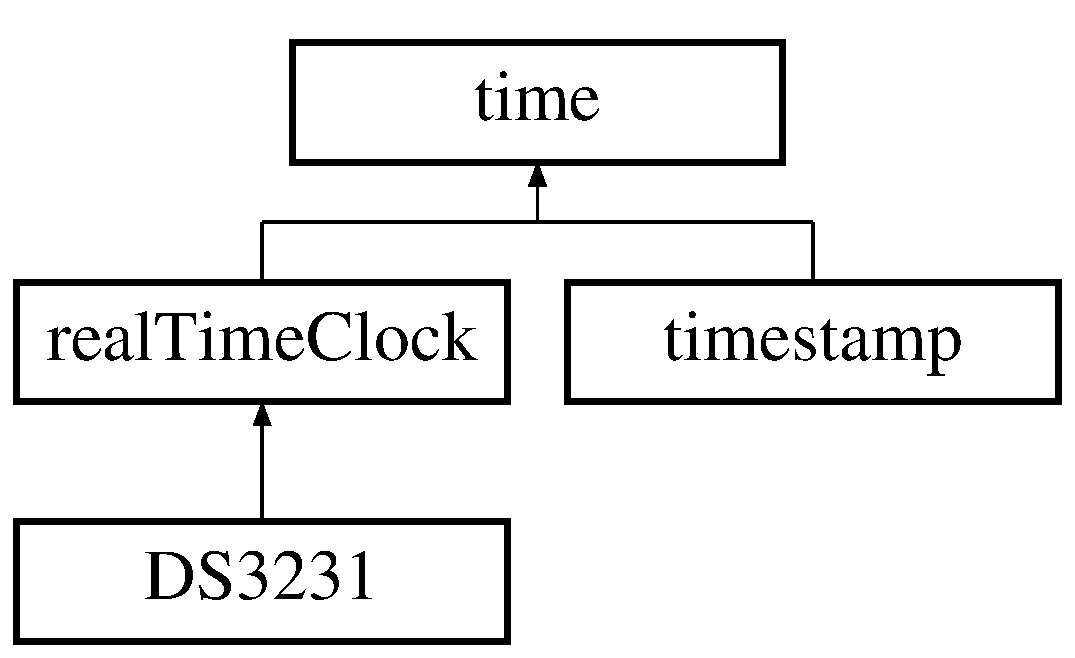
\includegraphics[height=3.000000cm]{classtime}
\end{center}
\end{figure}
\subsection*{Public Member Functions}
\begin{DoxyCompactItemize}
\item 
\mbox{\Hypertarget{classtime_aeba296b9c9c6ec09250f98a20062a500}\label{classtime_aeba296b9c9c6ec09250f98a20062a500}} 
bool {\bfseries is\+Seconds\+Valid} (uint8\+\_\+t seconds) const
\item 
\mbox{\Hypertarget{classtime_adafa6fb7a20aee5e865a51576ab9340b}\label{classtime_adafa6fb7a20aee5e865a51576ab9340b}} 
bool {\bfseries is\+Minutes\+Valid} (uint8\+\_\+t minutes) const
\item 
\mbox{\Hypertarget{classtime_afe3fbaa007cbc8072b36c8bd2a556365}\label{classtime_afe3fbaa007cbc8072b36c8bd2a556365}} 
bool {\bfseries is\+Hours\+Valid} (uint8\+\_\+t hours) const
\item 
\mbox{\Hypertarget{classtime_a126cf22d6b3a7a36603e2cb390082d2f}\label{classtime_a126cf22d6b3a7a36603e2cb390082d2f}} 
bool {\bfseries is\+Day\+Valid} (uint8\+\_\+t day) const
\item 
\mbox{\Hypertarget{classtime_aa678e8f53a12adda2f807e6a44ebc46d}\label{classtime_aa678e8f53a12adda2f807e6a44ebc46d}} 
bool {\bfseries is\+Date\+Valid} (uint8\+\_\+t date) const
\item 
\mbox{\Hypertarget{classtime_a92c265ce96b24f9bdfa960144a0bce11}\label{classtime_a92c265ce96b24f9bdfa960144a0bce11}} 
bool {\bfseries is\+Month\+Valid} (uint8\+\_\+t month) const
\item 
\mbox{\Hypertarget{classtime_ad6269d0f650cfc32e0ac83b09816abad}\label{classtime_ad6269d0f650cfc32e0ac83b09816abad}} 
bool {\bfseries is\+Year\+Valid} (uint8\+\_\+t year) const
\item 
\mbox{\Hypertarget{classtime_a01413b7e5754345cf032cc7afa13efb0}\label{classtime_a01413b7e5754345cf032cc7afa13efb0}} 
bool {\bfseries is\+Century\+Valid} (int century) const
\end{DoxyCompactItemize}
\subsection*{Static Public Member Functions}
\begin{DoxyCompactItemize}
\item 
\mbox{\Hypertarget{classtime_a35f54f331571b5bc8135f586045d753e}\label{classtime_a35f54f331571b5bc8135f586045d753e}} 
static void {\bfseries increase\+Century} ()
\end{DoxyCompactItemize}
\subsection*{Public Attributes}
\begin{DoxyCompactItemize}
\item 
\mbox{\Hypertarget{classtime_ab2b254fe96fb3bafed7da738bda3c6c6}\label{classtime_ab2b254fe96fb3bafed7da738bda3c6c6}} 
const uint8\+\_\+t {\bfseries min\+Seconds} = 0
\item 
\mbox{\Hypertarget{classtime_a23400f37b2c7f65ab8cc94059ec700f4}\label{classtime_a23400f37b2c7f65ab8cc94059ec700f4}} 
const uint8\+\_\+t {\bfseries min\+Minutes} = 0
\item 
\mbox{\Hypertarget{classtime_a92ca207c7e5ead60298ab7f3e1f9e002}\label{classtime_a92ca207c7e5ead60298ab7f3e1f9e002}} 
const uint8\+\_\+t {\bfseries min\+Date} = 0
\item 
\mbox{\Hypertarget{classtime_a1697927f878a6ff5b88a385ff1d13e32}\label{classtime_a1697927f878a6ff5b88a385ff1d13e32}} 
const uint8\+\_\+t {\bfseries min\+Year} = 0
\item 
\mbox{\Hypertarget{classtime_af5a330549db1f4a8f8576f0e2fbb8a49}\label{classtime_af5a330549db1f4a8f8576f0e2fbb8a49}} 
const uint8\+\_\+t {\bfseries min\+Hours} = 1
\item 
\mbox{\Hypertarget{classtime_af775686641b3f5a791e490c9e75a90d5}\label{classtime_af775686641b3f5a791e490c9e75a90d5}} 
const uint8\+\_\+t {\bfseries min\+Day} = 1
\item 
\mbox{\Hypertarget{classtime_a1a7dcc6e6ec193ec260b801598716d49}\label{classtime_a1a7dcc6e6ec193ec260b801598716d49}} 
const uint8\+\_\+t {\bfseries min\+Month} = 1
\item 
\mbox{\Hypertarget{classtime_ac2ce42c35a6dffe688f04edb3f02bba2}\label{classtime_ac2ce42c35a6dffe688f04edb3f02bba2}} 
const uint8\+\_\+t {\bfseries max\+Day} = 7
\item 
\mbox{\Hypertarget{classtime_a6bdfb853fd818812388132c32d13d58f}\label{classtime_a6bdfb853fd818812388132c32d13d58f}} 
const uint8\+\_\+t {\bfseries max\+Date} = 31
\item 
\mbox{\Hypertarget{classtime_a8659af00b37397c512e0215ca3c0de4c}\label{classtime_a8659af00b37397c512e0215ca3c0de4c}} 
const uint8\+\_\+t {\bfseries max\+Month} = 12
\item 
\mbox{\Hypertarget{classtime_a551d68c0f849a515c468f2e1ff08711a}\label{classtime_a551d68c0f849a515c468f2e1ff08711a}} 
const uint8\+\_\+t {\bfseries max\+Seconds} = 59
\item 
\mbox{\Hypertarget{classtime_a8cd18e83ca72f75a2e37176ba297c271}\label{classtime_a8cd18e83ca72f75a2e37176ba297c271}} 
const uint8\+\_\+t {\bfseries max\+Minutes} = 59
\item 
\mbox{\Hypertarget{classtime_a151534764ea356d9d9e7344a38b880ea}\label{classtime_a151534764ea356d9d9e7344a38b880ea}} 
const uint8\+\_\+t {\bfseries max\+Hours} = 23
\item 
\mbox{\Hypertarget{classtime_a0602061dd6152dc250b172580a175d9e}\label{classtime_a0602061dd6152dc250b172580a175d9e}} 
const uint8\+\_\+t {\bfseries max\+Year} = 99
\end{DoxyCompactItemize}
\subsection*{Static Public Attributes}
\begin{DoxyCompactItemize}
\item 
\mbox{\Hypertarget{classtime_acab6780ebb25862cb83316cb967b8b57}\label{classtime_acab6780ebb25862cb83316cb967b8b57}} 
static int {\bfseries current\+Century} = 2000
\end{DoxyCompactItemize}
\subsection*{Static Private Attributes}
\begin{DoxyCompactItemize}
\item 
\mbox{\Hypertarget{classtime_af12b7ed0d7ff922e00ecb46dabdaede6}\label{classtime_af12b7ed0d7ff922e00ecb46dabdaede6}} 
static const uint8\+\_\+t {\bfseries century\+Increase\+Value} = 100
\end{DoxyCompactItemize}


The documentation for this class was generated from the following files\+:\begin{DoxyCompactItemize}
\item 
Demo/time.\+hpp\item 
Demo/time.\+cpp\end{DoxyCompactItemize}

\hypertarget{classtimestamp}{}\section{timestamp Class Reference}
\label{classtimestamp}\index{timestamp@{timestamp}}


This class is used to store a timestamp. Using a timestamp makes it easier to store and get any time value.  




{\ttfamily \#include $<$timestamp.\+hpp$>$}

Inheritance diagram for timestamp\+:\begin{figure}[H]
\begin{center}
\leavevmode
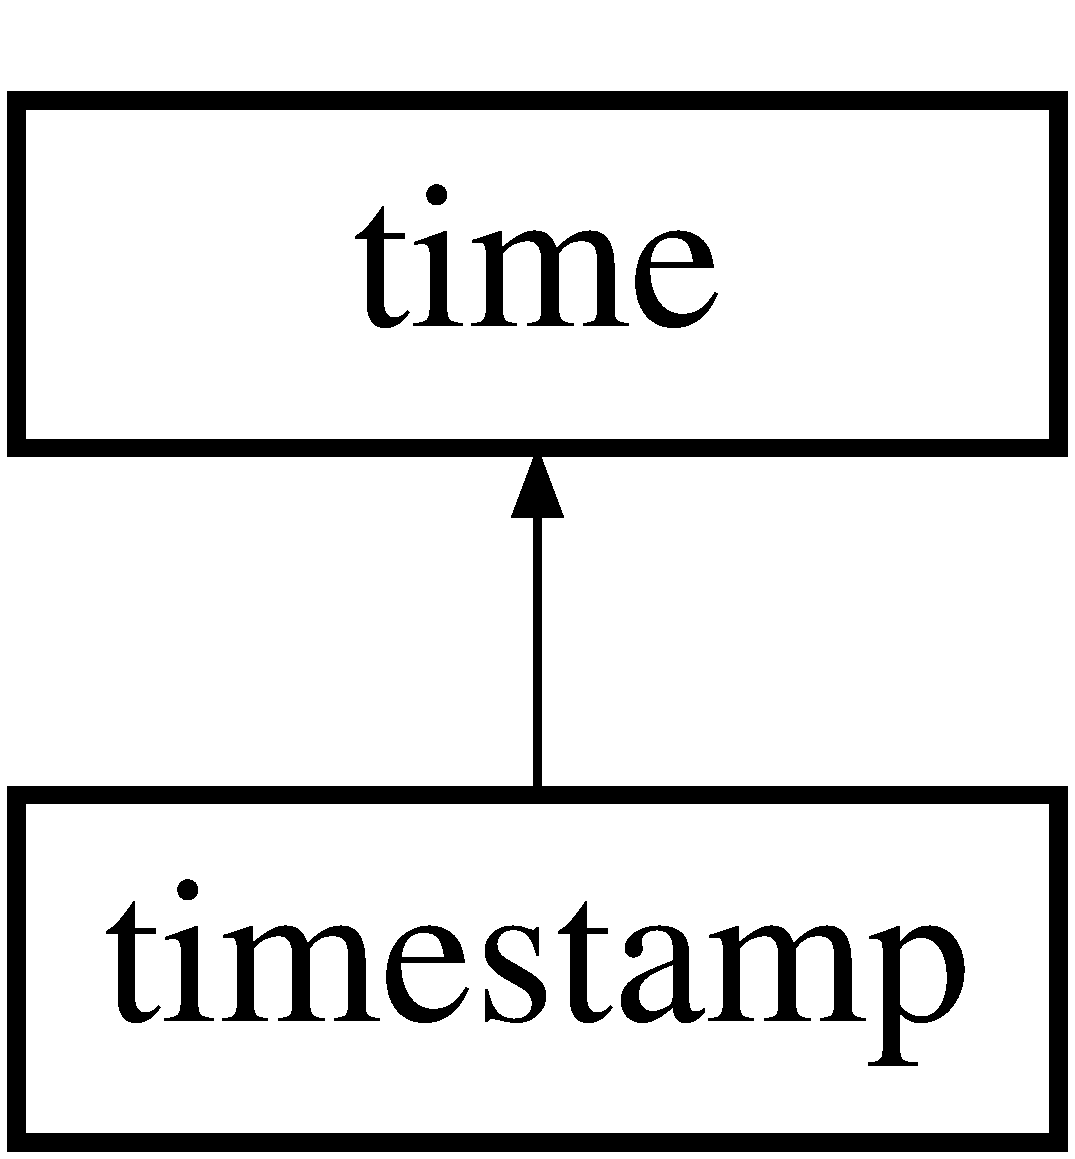
\includegraphics[height=2.000000cm]{classtimestamp}
\end{center}
\end{figure}
\subsection*{Public Member Functions}
\begin{DoxyCompactItemize}
\item 
\mbox{\hyperlink{classtimestamp_adcd43bf86d093792baa6b406e0acafd3}{timestamp}} (uint8\+\_\+t \mbox{\hyperlink{classtimestamp_a15ad236c6963bfbd6ae18416697c91c2}{seconds}}, uint8\+\_\+t \mbox{\hyperlink{classtimestamp_a45c06ef17b96bdd37cd168faf772c63c}{minutes}}, uint8\+\_\+t \mbox{\hyperlink{classtimestamp_a3b2f11626563cca00d60b323ceb15191}{hours}}, uint8\+\_\+t \mbox{\hyperlink{classtimestamp_a0102d6c44b2cc194a8186a42ff2bd58b}{day}}, uint8\+\_\+t \mbox{\hyperlink{classtimestamp_a7eb2eee5f6ef4258aab7779a639a93fd}{date}}, uint8\+\_\+t \mbox{\hyperlink{classtimestamp_a71df69b7ebb5a6dd228f4ae70b954505}{month}}, uint16\+\_\+t \mbox{\hyperlink{classtimestamp_a6df342bdd1101cf67f9a4831d5372d58}{year}})
\begin{DoxyCompactList}\small\item\em The constructor to set every variable in this class. \end{DoxyCompactList}\item 
\mbox{\hyperlink{classtimestamp_a155539f65cabcec4ed8120e7d531d92a}{timestamp}} ()
\begin{DoxyCompactList}\small\item\em The default constructor. \end{DoxyCompactList}\item 
void \mbox{\hyperlink{classtimestamp_a7d2a5311e064fb9fe0ebbb74e603091c}{set\+Seconds}} (uint8\+\_\+t new\+Seconds)
\begin{DoxyCompactList}\small\item\em Set the amount of seconds of the timestamp. \end{DoxyCompactList}\item 
uint8\+\_\+t \mbox{\hyperlink{classtimestamp_a9212a15c81b0f77b576257cba2805253}{get\+Seconds}} () const
\begin{DoxyCompactList}\small\item\em Get the value of \mbox{\hyperlink{classtimestamp_a15ad236c6963bfbd6ae18416697c91c2}{seconds}}. \end{DoxyCompactList}\item 
void \mbox{\hyperlink{classtimestamp_a95383562b21c79d2d3279f4c06a8cc18}{set\+Minutes}} (uint8\+\_\+t new\+Minutes)
\begin{DoxyCompactList}\small\item\em Set the amount of minutes of the timestamp. \end{DoxyCompactList}\item 
uint8\+\_\+t \mbox{\hyperlink{classtimestamp_a77adde4c8da3bfc1076882f2627938f7}{get\+Minutes}} () const
\begin{DoxyCompactList}\small\item\em Get the value of \mbox{\hyperlink{classtimestamp_a45c06ef17b96bdd37cd168faf772c63c}{minutes}}. \end{DoxyCompactList}\item 
void \mbox{\hyperlink{classtimestamp_ae074684cb0c1f937c9ab985692522217}{set\+Hours}} (uint8\+\_\+t new\+Hours)
\begin{DoxyCompactList}\small\item\em Set the amount of hours of the timestamp. \end{DoxyCompactList}\item 
uint8\+\_\+t \mbox{\hyperlink{classtimestamp_a9857c77d68def8f77737f3c3840b6b95}{get\+Hours}} () const
\begin{DoxyCompactList}\small\item\em Get the value of \mbox{\hyperlink{classtimestamp_a3b2f11626563cca00d60b323ceb15191}{hours}}. \end{DoxyCompactList}\item 
void \mbox{\hyperlink{classtimestamp_af280dd8ed37274b31a548619f21dddd9}{set\+Day}} (uint8\+\_\+t new\+Day)
\begin{DoxyCompactList}\small\item\em Set the the day of the timestamp. \end{DoxyCompactList}\item 
uint8\+\_\+t \mbox{\hyperlink{classtimestamp_a70baea53133ff4b05eb49332e3ef36bb}{get\+Day}} () const
\begin{DoxyCompactList}\small\item\em Get the value of \mbox{\hyperlink{classtimestamp_a0102d6c44b2cc194a8186a42ff2bd58b}{day}}. \end{DoxyCompactList}\item 
void \mbox{\hyperlink{classtimestamp_a7392ce4abda5f63e95462bd99691b719}{set\+Date}} (uint8\+\_\+t new\+Date)
\begin{DoxyCompactList}\small\item\em Set the the date of the timestamp. \end{DoxyCompactList}\item 
uint8\+\_\+t \mbox{\hyperlink{classtimestamp_a0ee0b3188b94fd8151f4525ea0de1078}{get\+Date}} () const
\begin{DoxyCompactList}\small\item\em Get the value of \mbox{\hyperlink{classtimestamp_a7eb2eee5f6ef4258aab7779a639a93fd}{date}}. \end{DoxyCompactList}\item 
void \mbox{\hyperlink{classtimestamp_ac95d923ad675c4a2bff8b4b0384b6222}{set\+Month}} (uint8\+\_\+t new\+Month)
\begin{DoxyCompactList}\small\item\em Set the the month of the timestamp. \end{DoxyCompactList}\item 
uint8\+\_\+t \mbox{\hyperlink{classtimestamp_a7225435b1a1ee20ae0dd8708f8e68ee8}{get\+Month}} () const
\begin{DoxyCompactList}\small\item\em Get the value of \mbox{\hyperlink{classtimestamp_a71df69b7ebb5a6dd228f4ae70b954505}{month}}. \end{DoxyCompactList}\item 
void \mbox{\hyperlink{classtimestamp_a2ad3d28f226c8f2ed74c06c609e29aff}{set\+Year}} (uint16\+\_\+t new\+Year)
\begin{DoxyCompactList}\small\item\em set the the year of the timestamp. \end{DoxyCompactList}\item 
uint8\+\_\+t \mbox{\hyperlink{classtimestamp_a21c6dd709bb29c95cea2641f26c6c088}{get\+Year}} () const
\begin{DoxyCompactList}\small\item\em Get the value of \mbox{\hyperlink{classtimestamp_a6df342bdd1101cf67f9a4831d5372d58}{year}}. \end{DoxyCompactList}\item 
void \mbox{\hyperlink{classtimestamp_ad7c219bebf2b101f13f0a48e435ad888}{set\+Century}} (int new\+Century)
\begin{DoxyCompactList}\small\item\em set the the century of the timestamp. \end{DoxyCompactList}\item 
int \mbox{\hyperlink{classtimestamp_a91ed1d395dd3d230607c4cb936b6004a}{get\+Century}} () const
\begin{DoxyCompactList}\small\item\em Get the value of \mbox{\hyperlink{classtimestamp_afe83888ffa38c1615a3d12b012f235b3}{century}}. \end{DoxyCompactList}\end{DoxyCompactItemize}
\subsection*{Protected Attributes}
\begin{DoxyCompactItemize}
\item 
\mbox{\Hypertarget{classtimestamp_a15ad236c6963bfbd6ae18416697c91c2}\label{classtimestamp_a15ad236c6963bfbd6ae18416697c91c2}} 
uint8\+\_\+t \mbox{\hyperlink{classtimestamp_a15ad236c6963bfbd6ae18416697c91c2}{seconds}}
\begin{DoxyCompactList}\small\item\em The seconds you want to store. (0 -\/ 59) \end{DoxyCompactList}\item 
\mbox{\Hypertarget{classtimestamp_a45c06ef17b96bdd37cd168faf772c63c}\label{classtimestamp_a45c06ef17b96bdd37cd168faf772c63c}} 
uint8\+\_\+t \mbox{\hyperlink{classtimestamp_a45c06ef17b96bdd37cd168faf772c63c}{minutes}}
\begin{DoxyCompactList}\small\item\em The minutes you want to store. (0 -\/ 59) \end{DoxyCompactList}\item 
\mbox{\Hypertarget{classtimestamp_a3b2f11626563cca00d60b323ceb15191}\label{classtimestamp_a3b2f11626563cca00d60b323ceb15191}} 
uint8\+\_\+t \mbox{\hyperlink{classtimestamp_a3b2f11626563cca00d60b323ceb15191}{hours}}
\begin{DoxyCompactList}\small\item\em The hours you want to store. (0 -\/ 23) \end{DoxyCompactList}\item 
\mbox{\Hypertarget{classtimestamp_a0102d6c44b2cc194a8186a42ff2bd58b}\label{classtimestamp_a0102d6c44b2cc194a8186a42ff2bd58b}} 
uint8\+\_\+t \mbox{\hyperlink{classtimestamp_a0102d6c44b2cc194a8186a42ff2bd58b}{day}}
\begin{DoxyCompactList}\small\item\em The hours you want to store. (1 = monday -\/ 7 = sunday) \end{DoxyCompactList}\item 
\mbox{\Hypertarget{classtimestamp_a7eb2eee5f6ef4258aab7779a639a93fd}\label{classtimestamp_a7eb2eee5f6ef4258aab7779a639a93fd}} 
uint8\+\_\+t \mbox{\hyperlink{classtimestamp_a7eb2eee5f6ef4258aab7779a639a93fd}{date}}
\begin{DoxyCompactList}\small\item\em The date you want to store. (0 -\/ 31) \end{DoxyCompactList}\item 
\mbox{\Hypertarget{classtimestamp_a71df69b7ebb5a6dd228f4ae70b954505}\label{classtimestamp_a71df69b7ebb5a6dd228f4ae70b954505}} 
uint8\+\_\+t \mbox{\hyperlink{classtimestamp_a71df69b7ebb5a6dd228f4ae70b954505}{month}}
\begin{DoxyCompactList}\small\item\em The month you want to store. (1 -\/ 12) \end{DoxyCompactList}\item 
uint8\+\_\+t \mbox{\hyperlink{classtimestamp_a6df342bdd1101cf67f9a4831d5372d58}{year}}
\begin{DoxyCompactList}\small\item\em The year you want to store. (0 -\/ 99) \end{DoxyCompactList}\item 
int \mbox{\hyperlink{classtimestamp_afe83888ffa38c1615a3d12b012f235b3}{century}}
\begin{DoxyCompactList}\small\item\em The century you want to store. \end{DoxyCompactList}\end{DoxyCompactItemize}
\subsection*{Friends}
\begin{DoxyCompactItemize}
\item 
hwlib\+::ostream \& \mbox{\hyperlink{classtimestamp_a0625abe0748dbab228b73920dfc33c4c}{operator$<$$<$}} (hwlib\+::ostream \&lhs, const \mbox{\hyperlink{classtimestamp}{timestamp}} \&rhs)
\begin{DoxyCompactList}\small\item\em Send the current timestamp to an ostream. \end{DoxyCompactList}\end{DoxyCompactItemize}
\subsection*{Additional Inherited Members}


\subsection{Detailed Description}
This class is used to store a timestamp. Using a timestamp makes it easier to store and get any time value. 

This timestamp is made to make it easier for the user to store a given point in time. The class checks the values before storing for extra safety. \begin{DoxyWarning}{Warning}
T\+HE S\+O\+F\+T\+W\+A\+RE IS P\+R\+O\+V\+I\+D\+ED \char`\"{}\+A\+S I\+S\char`\"{}, W\+I\+T\+H\+O\+UT W\+A\+R\+R\+A\+N\+TY OF A\+NY K\+I\+ND. 
\end{DoxyWarning}


\subsection{Constructor \& Destructor Documentation}
\mbox{\Hypertarget{classtimestamp_adcd43bf86d093792baa6b406e0acafd3}\label{classtimestamp_adcd43bf86d093792baa6b406e0acafd3}} 
\index{timestamp@{timestamp}!timestamp@{timestamp}}
\index{timestamp@{timestamp}!timestamp@{timestamp}}
\subsubsection{\texorpdfstring{timestamp()}{timestamp()}\hspace{0.1cm}{\footnotesize\ttfamily [1/2]}}
{\footnotesize\ttfamily timestamp\+::timestamp (\begin{DoxyParamCaption}\item[{uint8\+\_\+t}]{seconds,  }\item[{uint8\+\_\+t}]{minutes,  }\item[{uint8\+\_\+t}]{hours,  }\item[{uint8\+\_\+t}]{day,  }\item[{uint8\+\_\+t}]{date,  }\item[{uint8\+\_\+t}]{month,  }\item[{uint16\+\_\+t}]{year }\end{DoxyParamCaption})}



The constructor to set every variable in this class. 

I recommend using this constructor when you already know the values you want to store. When you use the default constructor every variable will set to the minimum value. ~\newline
 \begin{DoxySeeAlso}{See also}
For the minimum values check \mbox{\hyperlink{time_8hpp_source}{time.\+hpp}}. 
\end{DoxySeeAlso}
\mbox{\Hypertarget{classtimestamp_a155539f65cabcec4ed8120e7d531d92a}\label{classtimestamp_a155539f65cabcec4ed8120e7d531d92a}} 
\index{timestamp@{timestamp}!timestamp@{timestamp}}
\index{timestamp@{timestamp}!timestamp@{timestamp}}
\subsubsection{\texorpdfstring{timestamp()}{timestamp()}\hspace{0.1cm}{\footnotesize\ttfamily [2/2]}}
{\footnotesize\ttfamily timestamp\+::timestamp (\begin{DoxyParamCaption}{ }\end{DoxyParamCaption})}



The default constructor. 

Every variable will set to the minimum value. ~\newline
 \begin{DoxySeeAlso}{See also}
For the minimum values check \mbox{\hyperlink{time_8hpp_source}{time.\+hpp}}. 
\end{DoxySeeAlso}


\subsection{Member Function Documentation}
\mbox{\Hypertarget{classtimestamp_a91ed1d395dd3d230607c4cb936b6004a}\label{classtimestamp_a91ed1d395dd3d230607c4cb936b6004a}} 
\index{timestamp@{timestamp}!get\+Century@{get\+Century}}
\index{get\+Century@{get\+Century}!timestamp@{timestamp}}
\subsubsection{\texorpdfstring{get\+Century()}{getCentury()}}
{\footnotesize\ttfamily int timestamp\+::get\+Century (\begin{DoxyParamCaption}{ }\end{DoxyParamCaption}) const}



Get the value of \mbox{\hyperlink{classtimestamp_afe83888ffa38c1615a3d12b012f235b3}{century}}. 

\begin{DoxyReturn}{Returns}
An int containing the value of \mbox{\hyperlink{classtimestamp_afe83888ffa38c1615a3d12b012f235b3}{century}}. 
\end{DoxyReturn}
\mbox{\Hypertarget{classtimestamp_a0ee0b3188b94fd8151f4525ea0de1078}\label{classtimestamp_a0ee0b3188b94fd8151f4525ea0de1078}} 
\index{timestamp@{timestamp}!get\+Date@{get\+Date}}
\index{get\+Date@{get\+Date}!timestamp@{timestamp}}
\subsubsection{\texorpdfstring{get\+Date()}{getDate()}}
{\footnotesize\ttfamily uint8\+\_\+t timestamp\+::get\+Date (\begin{DoxyParamCaption}{ }\end{DoxyParamCaption}) const}



Get the value of \mbox{\hyperlink{classtimestamp_a7eb2eee5f6ef4258aab7779a639a93fd}{date}}. 

\begin{DoxyReturn}{Returns}
An uint8\+\_\+t containing the value of \mbox{\hyperlink{classtimestamp_a7eb2eee5f6ef4258aab7779a639a93fd}{date}}. 
\end{DoxyReturn}
\mbox{\Hypertarget{classtimestamp_a70baea53133ff4b05eb49332e3ef36bb}\label{classtimestamp_a70baea53133ff4b05eb49332e3ef36bb}} 
\index{timestamp@{timestamp}!get\+Day@{get\+Day}}
\index{get\+Day@{get\+Day}!timestamp@{timestamp}}
\subsubsection{\texorpdfstring{get\+Day()}{getDay()}}
{\footnotesize\ttfamily uint8\+\_\+t timestamp\+::get\+Day (\begin{DoxyParamCaption}{ }\end{DoxyParamCaption}) const}



Get the value of \mbox{\hyperlink{classtimestamp_a0102d6c44b2cc194a8186a42ff2bd58b}{day}}. 

\begin{DoxyReturn}{Returns}
An uint8\+\_\+t containing the value of \mbox{\hyperlink{classtimestamp_a0102d6c44b2cc194a8186a42ff2bd58b}{day}}. 
\end{DoxyReturn}
\mbox{\Hypertarget{classtimestamp_a9857c77d68def8f77737f3c3840b6b95}\label{classtimestamp_a9857c77d68def8f77737f3c3840b6b95}} 
\index{timestamp@{timestamp}!get\+Hours@{get\+Hours}}
\index{get\+Hours@{get\+Hours}!timestamp@{timestamp}}
\subsubsection{\texorpdfstring{get\+Hours()}{getHours()}}
{\footnotesize\ttfamily uint8\+\_\+t timestamp\+::get\+Hours (\begin{DoxyParamCaption}{ }\end{DoxyParamCaption}) const}



Get the value of \mbox{\hyperlink{classtimestamp_a3b2f11626563cca00d60b323ceb15191}{hours}}. 

\begin{DoxyReturn}{Returns}
An uint8\+\_\+t containing the value of \mbox{\hyperlink{classtimestamp_a3b2f11626563cca00d60b323ceb15191}{hours}}. 
\end{DoxyReturn}
\mbox{\Hypertarget{classtimestamp_a77adde4c8da3bfc1076882f2627938f7}\label{classtimestamp_a77adde4c8da3bfc1076882f2627938f7}} 
\index{timestamp@{timestamp}!get\+Minutes@{get\+Minutes}}
\index{get\+Minutes@{get\+Minutes}!timestamp@{timestamp}}
\subsubsection{\texorpdfstring{get\+Minutes()}{getMinutes()}}
{\footnotesize\ttfamily uint8\+\_\+t timestamp\+::get\+Minutes (\begin{DoxyParamCaption}{ }\end{DoxyParamCaption}) const}



Get the value of \mbox{\hyperlink{classtimestamp_a45c06ef17b96bdd37cd168faf772c63c}{minutes}}. 

\begin{DoxyReturn}{Returns}
An uint8\+\_\+t containing the value of \mbox{\hyperlink{classtimestamp_a45c06ef17b96bdd37cd168faf772c63c}{minutes}}. 
\end{DoxyReturn}
\mbox{\Hypertarget{classtimestamp_a7225435b1a1ee20ae0dd8708f8e68ee8}\label{classtimestamp_a7225435b1a1ee20ae0dd8708f8e68ee8}} 
\index{timestamp@{timestamp}!get\+Month@{get\+Month}}
\index{get\+Month@{get\+Month}!timestamp@{timestamp}}
\subsubsection{\texorpdfstring{get\+Month()}{getMonth()}}
{\footnotesize\ttfamily uint8\+\_\+t timestamp\+::get\+Month (\begin{DoxyParamCaption}{ }\end{DoxyParamCaption}) const}



Get the value of \mbox{\hyperlink{classtimestamp_a71df69b7ebb5a6dd228f4ae70b954505}{month}}. 

\begin{DoxyReturn}{Returns}
An uint8\+\_\+t containing the value of \mbox{\hyperlink{classtimestamp_a71df69b7ebb5a6dd228f4ae70b954505}{month}}. 
\end{DoxyReturn}
\mbox{\Hypertarget{classtimestamp_a9212a15c81b0f77b576257cba2805253}\label{classtimestamp_a9212a15c81b0f77b576257cba2805253}} 
\index{timestamp@{timestamp}!get\+Seconds@{get\+Seconds}}
\index{get\+Seconds@{get\+Seconds}!timestamp@{timestamp}}
\subsubsection{\texorpdfstring{get\+Seconds()}{getSeconds()}}
{\footnotesize\ttfamily uint8\+\_\+t timestamp\+::get\+Seconds (\begin{DoxyParamCaption}{ }\end{DoxyParamCaption}) const}



Get the value of \mbox{\hyperlink{classtimestamp_a15ad236c6963bfbd6ae18416697c91c2}{seconds}}. 

\begin{DoxyReturn}{Returns}
An uint8\+\_\+t containing the value of \mbox{\hyperlink{classtimestamp_a15ad236c6963bfbd6ae18416697c91c2}{seconds}}. 
\end{DoxyReturn}
\mbox{\Hypertarget{classtimestamp_a21c6dd709bb29c95cea2641f26c6c088}\label{classtimestamp_a21c6dd709bb29c95cea2641f26c6c088}} 
\index{timestamp@{timestamp}!get\+Year@{get\+Year}}
\index{get\+Year@{get\+Year}!timestamp@{timestamp}}
\subsubsection{\texorpdfstring{get\+Year()}{getYear()}}
{\footnotesize\ttfamily uint8\+\_\+t timestamp\+::get\+Year (\begin{DoxyParamCaption}{ }\end{DoxyParamCaption}) const}



Get the value of \mbox{\hyperlink{classtimestamp_a6df342bdd1101cf67f9a4831d5372d58}{year}}. 

\begin{DoxyReturn}{Returns}
An uint8\+\_\+t containing the value of \mbox{\hyperlink{classtimestamp_a6df342bdd1101cf67f9a4831d5372d58}{year}}. 
\end{DoxyReturn}
\mbox{\Hypertarget{classtimestamp_ad7c219bebf2b101f13f0a48e435ad888}\label{classtimestamp_ad7c219bebf2b101f13f0a48e435ad888}} 
\index{timestamp@{timestamp}!set\+Century@{set\+Century}}
\index{set\+Century@{set\+Century}!timestamp@{timestamp}}
\subsubsection{\texorpdfstring{set\+Century()}{setCentury()}}
{\footnotesize\ttfamily void timestamp\+::set\+Century (\begin{DoxyParamCaption}\item[{int}]{new\+Century }\end{DoxyParamCaption})}



set the the century of the timestamp. 


\begin{DoxyParams}{Parameters}
{\em new\+Century} & the the century you want to store in \mbox{\hyperlink{classtimestamp_afe83888ffa38c1615a3d12b012f235b3}{century}}.\\
\hline
\end{DoxyParams}
Before setting the value in \mbox{\hyperlink{classtimestamp_afe83888ffa38c1615a3d12b012f235b3}{century}}, new\+Century is checked. Using a function in \mbox{\hyperlink{time_8hpp_source}{time.\+hpp}} \begin{DoxySeeAlso}{See also}
\mbox{\hyperlink{classtime_a01413b7e5754345cf032cc7afa13efb0}{time\+::is\+Century\+Valid}} 
\end{DoxySeeAlso}
\mbox{\Hypertarget{classtimestamp_a7392ce4abda5f63e95462bd99691b719}\label{classtimestamp_a7392ce4abda5f63e95462bd99691b719}} 
\index{timestamp@{timestamp}!set\+Date@{set\+Date}}
\index{set\+Date@{set\+Date}!timestamp@{timestamp}}
\subsubsection{\texorpdfstring{set\+Date()}{setDate()}}
{\footnotesize\ttfamily void timestamp\+::set\+Date (\begin{DoxyParamCaption}\item[{uint8\+\_\+t}]{new\+Date }\end{DoxyParamCaption})}



Set the the date of the timestamp. 


\begin{DoxyParams}{Parameters}
{\em new\+Date} & the the date you want to store in \mbox{\hyperlink{classtimestamp_a7eb2eee5f6ef4258aab7779a639a93fd}{date}}.\\
\hline
\end{DoxyParams}
Before setting the value in \mbox{\hyperlink{classtimestamp_a7eb2eee5f6ef4258aab7779a639a93fd}{date}}, new\+Date is checked. Using a function in \mbox{\hyperlink{time_8hpp_source}{time.\+hpp}} \begin{DoxySeeAlso}{See also}
\mbox{\hyperlink{classtime_aa678e8f53a12adda2f807e6a44ebc46d}{time\+::is\+Date\+Valid}} 
\end{DoxySeeAlso}
\mbox{\Hypertarget{classtimestamp_af280dd8ed37274b31a548619f21dddd9}\label{classtimestamp_af280dd8ed37274b31a548619f21dddd9}} 
\index{timestamp@{timestamp}!set\+Day@{set\+Day}}
\index{set\+Day@{set\+Day}!timestamp@{timestamp}}
\subsubsection{\texorpdfstring{set\+Day()}{setDay()}}
{\footnotesize\ttfamily void timestamp\+::set\+Day (\begin{DoxyParamCaption}\item[{uint8\+\_\+t}]{new\+Day }\end{DoxyParamCaption})}



Set the the day of the timestamp. 


\begin{DoxyParams}{Parameters}
{\em new\+Day} & the the day you want to store in \mbox{\hyperlink{classtimestamp_a0102d6c44b2cc194a8186a42ff2bd58b}{day}}.\\
\hline
\end{DoxyParams}
Before setting the value in \mbox{\hyperlink{classtimestamp_a0102d6c44b2cc194a8186a42ff2bd58b}{day}}, new\+Day is checked. Using a function in \mbox{\hyperlink{time_8hpp_source}{time.\+hpp}} \begin{DoxySeeAlso}{See also}
\mbox{\hyperlink{classtime_a126cf22d6b3a7a36603e2cb390082d2f}{time\+::is\+Day\+Valid}} 
\end{DoxySeeAlso}
\mbox{\Hypertarget{classtimestamp_ae074684cb0c1f937c9ab985692522217}\label{classtimestamp_ae074684cb0c1f937c9ab985692522217}} 
\index{timestamp@{timestamp}!set\+Hours@{set\+Hours}}
\index{set\+Hours@{set\+Hours}!timestamp@{timestamp}}
\subsubsection{\texorpdfstring{set\+Hours()}{setHours()}}
{\footnotesize\ttfamily void timestamp\+::set\+Hours (\begin{DoxyParamCaption}\item[{uint8\+\_\+t}]{new\+Hours }\end{DoxyParamCaption})}



Set the amount of hours of the timestamp. 


\begin{DoxyParams}{Parameters}
{\em new\+Hours} & the amount of hours you want to store in \mbox{\hyperlink{classtimestamp_a3b2f11626563cca00d60b323ceb15191}{hours}}.\\
\hline
\end{DoxyParams}
Before setting the value in \mbox{\hyperlink{classtimestamp_a3b2f11626563cca00d60b323ceb15191}{hours}}, new\+Hours is checked. Using a function in \mbox{\hyperlink{time_8hpp_source}{time.\+hpp}} \begin{DoxySeeAlso}{See also}
\mbox{\hyperlink{classtime_afe3fbaa007cbc8072b36c8bd2a556365}{time\+::is\+Hours\+Valid}} 
\end{DoxySeeAlso}
\mbox{\Hypertarget{classtimestamp_a95383562b21c79d2d3279f4c06a8cc18}\label{classtimestamp_a95383562b21c79d2d3279f4c06a8cc18}} 
\index{timestamp@{timestamp}!set\+Minutes@{set\+Minutes}}
\index{set\+Minutes@{set\+Minutes}!timestamp@{timestamp}}
\subsubsection{\texorpdfstring{set\+Minutes()}{setMinutes()}}
{\footnotesize\ttfamily void timestamp\+::set\+Minutes (\begin{DoxyParamCaption}\item[{uint8\+\_\+t}]{new\+Minutes }\end{DoxyParamCaption})}



Set the amount of minutes of the timestamp. 


\begin{DoxyParams}{Parameters}
{\em new\+Minutes} & the amount of minutes you want to store in \mbox{\hyperlink{classtimestamp_a45c06ef17b96bdd37cd168faf772c63c}{minutes}}.\\
\hline
\end{DoxyParams}
Before setting the value in \mbox{\hyperlink{classtimestamp_a45c06ef17b96bdd37cd168faf772c63c}{minutes}}, new\+Minutes is checked. Using a function in \mbox{\hyperlink{time_8hpp_source}{time.\+hpp}} \begin{DoxySeeAlso}{See also}
\mbox{\hyperlink{classtime_adafa6fb7a20aee5e865a51576ab9340b}{time\+::is\+Minutes\+Valid}} 
\end{DoxySeeAlso}
\mbox{\Hypertarget{classtimestamp_ac95d923ad675c4a2bff8b4b0384b6222}\label{classtimestamp_ac95d923ad675c4a2bff8b4b0384b6222}} 
\index{timestamp@{timestamp}!set\+Month@{set\+Month}}
\index{set\+Month@{set\+Month}!timestamp@{timestamp}}
\subsubsection{\texorpdfstring{set\+Month()}{setMonth()}}
{\footnotesize\ttfamily void timestamp\+::set\+Month (\begin{DoxyParamCaption}\item[{uint8\+\_\+t}]{new\+Month }\end{DoxyParamCaption})}



Set the the month of the timestamp. 


\begin{DoxyParams}{Parameters}
{\em new\+Month} & the the month you want to store in \mbox{\hyperlink{classtimestamp_a71df69b7ebb5a6dd228f4ae70b954505}{month}}.\\
\hline
\end{DoxyParams}
Before setting the value in \mbox{\hyperlink{classtimestamp_a71df69b7ebb5a6dd228f4ae70b954505}{month}}, new\+Month is checked. Using a function in \mbox{\hyperlink{time_8hpp_source}{time.\+hpp}} \begin{DoxySeeAlso}{See also}
\mbox{\hyperlink{classtime_a92c265ce96b24f9bdfa960144a0bce11}{time\+::is\+Month\+Valid}} 
\end{DoxySeeAlso}
\mbox{\Hypertarget{classtimestamp_a7d2a5311e064fb9fe0ebbb74e603091c}\label{classtimestamp_a7d2a5311e064fb9fe0ebbb74e603091c}} 
\index{timestamp@{timestamp}!set\+Seconds@{set\+Seconds}}
\index{set\+Seconds@{set\+Seconds}!timestamp@{timestamp}}
\subsubsection{\texorpdfstring{set\+Seconds()}{setSeconds()}}
{\footnotesize\ttfamily void timestamp\+::set\+Seconds (\begin{DoxyParamCaption}\item[{uint8\+\_\+t}]{new\+Seconds }\end{DoxyParamCaption})}



Set the amount of seconds of the timestamp. 


\begin{DoxyParams}{Parameters}
{\em new\+Seconds} & the amount of seconds you want to store in \mbox{\hyperlink{classtimestamp_a15ad236c6963bfbd6ae18416697c91c2}{seconds}}.\\
\hline
\end{DoxyParams}
Before setting the value in \mbox{\hyperlink{classtimestamp_a15ad236c6963bfbd6ae18416697c91c2}{seconds}}, new\+Seconds is checked. Using a function in \mbox{\hyperlink{time_8hpp_source}{time.\+hpp}} \begin{DoxySeeAlso}{See also}
\mbox{\hyperlink{classtime_aeba296b9c9c6ec09250f98a20062a500}{time\+::is\+Seconds\+Valid}} 
\end{DoxySeeAlso}
\mbox{\Hypertarget{classtimestamp_a2ad3d28f226c8f2ed74c06c609e29aff}\label{classtimestamp_a2ad3d28f226c8f2ed74c06c609e29aff}} 
\index{timestamp@{timestamp}!set\+Year@{set\+Year}}
\index{set\+Year@{set\+Year}!timestamp@{timestamp}}
\subsubsection{\texorpdfstring{set\+Year()}{setYear()}}
{\footnotesize\ttfamily void timestamp\+::set\+Year (\begin{DoxyParamCaption}\item[{uint16\+\_\+t}]{new\+Year }\end{DoxyParamCaption})}



set the the year of the timestamp. 


\begin{DoxyParams}{Parameters}
{\em new\+Year} & the the year you want to store in \mbox{\hyperlink{classtimestamp_a6df342bdd1101cf67f9a4831d5372d58}{year}}.\\
\hline
\end{DoxyParams}
Before setting the value in \mbox{\hyperlink{classtimestamp_a6df342bdd1101cf67f9a4831d5372d58}{year}}, new\+Year is checked. Using a function in \mbox{\hyperlink{time_8hpp_source}{time.\+hpp}} \begin{DoxySeeAlso}{See also}
\mbox{\hyperlink{classtime_ad6269d0f650cfc32e0ac83b09816abad}{time\+::is\+Year\+Valid}} 
\end{DoxySeeAlso}


\subsection{Friends And Related Function Documentation}
\mbox{\Hypertarget{classtimestamp_a0625abe0748dbab228b73920dfc33c4c}\label{classtimestamp_a0625abe0748dbab228b73920dfc33c4c}} 
\index{timestamp@{timestamp}!operator$<$$<$@{operator$<$$<$}}
\index{operator$<$$<$@{operator$<$$<$}!timestamp@{timestamp}}
\subsubsection{\texorpdfstring{operator$<$$<$}{operator<<}}
{\footnotesize\ttfamily hwlib\+::ostream\& operator$<$$<$ (\begin{DoxyParamCaption}\item[{hwlib\+::ostream \&}]{lhs,  }\item[{const \mbox{\hyperlink{classtimestamp}{timestamp}} \&}]{rhs }\end{DoxyParamCaption})\hspace{0.3cm}{\ttfamily [friend]}}



Send the current timestamp to an ostream. 


\begin{DoxyParams}{Parameters}
{\em lhs} & the ostream you want to change. \\
\hline
{\em rhs} & the timestamp you want to set in the ostream. (lhs) \\
\hline
\end{DoxyParams}
\begin{DoxyReturn}{Returns}
A hwlib\+::ostream (\href{mailto:wouter@voti.nl}{\tt wouter@voti.\+nl} 2017) containing the previous values and the timestamp.
\end{DoxyReturn}
This method is used to for example print a timestamp the simple way. \begin{DoxyWarning}{Warning}
Note that the given ostream will be changed during the execution. 
\end{DoxyWarning}


\subsection{Member Data Documentation}
\mbox{\Hypertarget{classtimestamp_afe83888ffa38c1615a3d12b012f235b3}\label{classtimestamp_afe83888ffa38c1615a3d12b012f235b3}} 
\index{timestamp@{timestamp}!century@{century}}
\index{century@{century}!timestamp@{timestamp}}
\subsubsection{\texorpdfstring{century}{century}}
{\footnotesize\ttfamily int timestamp\+::century\hspace{0.3cm}{\ttfamily [protected]}}



The century you want to store. 

The century will be set using the \mbox{\hyperlink{classtime_acab6780ebb25862cb83316cb967b8b57}{time\+::current\+Century}} variable. \mbox{\Hypertarget{classtimestamp_a6df342bdd1101cf67f9a4831d5372d58}\label{classtimestamp_a6df342bdd1101cf67f9a4831d5372d58}} 
\index{timestamp@{timestamp}!year@{year}}
\index{year@{year}!timestamp@{timestamp}}
\subsubsection{\texorpdfstring{year}{year}}
{\footnotesize\ttfamily uint8\+\_\+t timestamp\+::year\hspace{0.3cm}{\ttfamily [protected]}}



The year you want to store. (0 -\/ 99) 

\begin{DoxyWarning}{Warning}
Note that the value ranges between 0 -\/ 99. The century is store in another variable \mbox{\hyperlink{classtimestamp_afe83888ffa38c1615a3d12b012f235b3}{century}}. 
\end{DoxyWarning}


The documentation for this class was generated from the following files\+:\begin{DoxyCompactItemize}
\item 
Demo/timestamp.\+hpp\item 
Demo/timestamp.\+cpp\end{DoxyCompactItemize}

%--- End generated contents ---

% Index
\backmatter
\newpage
\phantomsection
\clearemptydoublepage
\addcontentsline{toc}{chapter}{Index}
\printindex

\end{document}
